\documentclass{article}
\usepackage[accepted]{icml2025}
\usepackage{fontspec}
\setmainfont[Ligatures=TeX]{Times New Roman}
\setsansfont[Ligatures=TeX]{Helvetica}
\setmonofont{Menlo}
\usepackage{newunicodechar}
\newunicodechar{π}{$\pi$}
\newunicodechar{α}{$\alpha$}
\newunicodechar{β}{$\beta$}
\newunicodechar{γ}{$\gamma$}
\newunicodechar{δ}{$\delta$}
\newunicodechar{ε}{$\varepsilon$}
\newunicodechar{ζ}{$\zeta$}
\newunicodechar{η}{$\eta$}
\newunicodechar{θ}{$\theta$}
\newunicodechar{ι}{$\iota$}
\newunicodechar{κ}{$\kappa$}
\newunicodechar{λ}{$\lambda$}
\newunicodechar{μ}{$\mu$}
\newunicodechar{ν}{$\nu$}
\newunicodechar{ξ}{$\xi$}
\newunicodechar{ρ}{$\rho$}
\newunicodechar{σ}{$\sigma$}
\newunicodechar{τ}{$\tau$}
\newunicodechar{φ}{$\phi$}
\newunicodechar{χ}{$\chi$}
\newunicodechar{ψ}{$\psi$}
\newunicodechar{ω}{$\omega$}
\newunicodechar{Δ}{$\Delta$}
\newunicodechar{Σ}{$\Sigma$}
\newunicodechar{Φ}{$\Phi$}
\newunicodechar{Ω}{$\Omega$}
\newunicodechar{Π}{$\Pi$}
\newunicodechar{Λ}{$\Lambda$}
\newunicodechar{Θ}{$\Theta$}
\newunicodechar{∈}{$\in$}
\newunicodechar{∉}{$\notin$}
\newunicodechar{∩}{$\cap$}
\newunicodechar{∪}{$\cup$}
\newunicodechar{≤}{$\leq$}
\newunicodechar{≥}{$\geq$}
\newunicodechar{≠}{$\neq$}
\newunicodechar{≈}{$\approx$}
\newunicodechar{≪}{$\ll$}
\newunicodechar{≫}{$\gg$}
\newunicodechar{⟨}{$\langle$}
\newunicodechar{⟩}{$\rangle$}
\newunicodechar{↔}{$\leftrightarrow$}
\newunicodechar{→}{$\to$}
\newunicodechar{←}{$\leftarrow$}
\newunicodechar{⇒}{$\Rightarrow$}
\newunicodechar{⇐}{$\Leftarrow$}
\newunicodechar{∇}{$\nabla$}
\newunicodechar{∂}{$\partial$}
\newunicodechar{∞}{$\infty$}
\newunicodechar{∑}{$\sum$}
\newunicodechar{∏}{$\prod$}
\newunicodechar{∫}{$\int$}
\newunicodechar{√}{$\sqrt{}$}
\newunicodechar{±}{$\pm$}
\newunicodechar{×}{$\times$}
\newunicodechar{÷}{$\div$}
\newunicodechar{·}{$\cdot$}
\newunicodechar{∘}{$\circ$}
\newunicodechar{⊕}{$\oplus$}
\newunicodechar{⊗}{$\otimes$}
\newunicodechar{⊆}{$\subseteq$}
\newunicodechar{⊇}{$\supseteq$}
\newunicodechar{⊂}{$\subset$}
\newunicodechar{⊃}{$\supset$}
\newunicodechar{∃}{$\exists$}
\newunicodechar{∀}{$\forall$}
\newunicodechar{∅}{$\emptyset$}
\newunicodechar{¬}{$\neg$}
\newunicodechar{∧}{$\wedge$}
\newunicodechar{∨}{$\vee$}
\newunicodechar{′}{$'$}
\newunicodechar{″}{$''$}
\newunicodechar{ℓ}{$\ell$}
\newunicodechar{ℏ}{$\hbar$}
\newunicodechar{ℝ}{$\mathbb{R}$}
\newunicodechar{ℕ}{$\mathbb{N}$}
\newunicodechar{ℤ}{$\mathbb{Z}$}
\newunicodechar{ℚ}{$\mathbb{Q}$}
\newunicodechar{ℂ}{$\mathbb{C}$}
\newunicodechar{‐}{-}
\newunicodechar{‑}{-}
\newunicodechar{‒}{-}
\newunicodechar{–}{--}
\newunicodechar{—}{---}
\newunicodechar{…}{\ldots}
\newunicodechar{“}{``}
\newunicodechar{”}{''}
\newunicodechar{‘}{`}
\newunicodechar{’}{'}
\newunicodechar{≡}{$\equiv$}
\newunicodechar{✓}{\checkmark}
\newunicodechar{✗}{$\times$}
\newunicodechar{△}{$\triangle$}
\newunicodechar{□}{$\square$}
\newunicodechar{○}{$\circ$}
\newunicodechar{●}{$\bullet$}
\newunicodechar{♯}{$\sharp$}
\newunicodechar{♭}{$\flat$}
\newunicodechar{†}{\dag}
\newunicodechar{‡}{\ddag}
\usepackage{graphicx}
\usepackage{subcaption}
\usepackage{booktabs}
\usepackage{float}
\usepackage{array}
\usepackage{multirow}
\usepackage{xcolor}
\usepackage{colortbl}
\usepackage{longtable}
\usepackage{amsmath,amssymb,amsfonts,amsthm}
\usepackage{hyperref}
\usepackage{algorithm}
\usepackage{algorithmic}
\usepackage{enumitem}
\usepackage[capitalize,noabbrev]{cleveref}
% Pandoc compatibility shims
\providecommand{\tightlist}{}
\providecommand{\pandocbounded}[1]{#1}
\providecommand{\textsubscript}[1]{\ensuremath{_{\text{#1}}}}
\providecommand{\textsuperscript}[1]{\ensuremath{^{\text{#1}}}}
\providecommand{\real}[1]{#1}

\providecommand{\passthrough}[1]{#1}

% Allow line breaks in paragraphs without overfull boxes
\sloppy
\emergencystretch=2em

\icmltitlerunning{Multimodal Large Language Models}

\begin{document}

\twocolumn[
  \icmltitle{Multimodal Large Language Models}

  \icmlsetsymbol{equal}{*}

  \begin{icmlauthorlist}
    \icmlauthor{Anonymous}{anon}
  \end{icmlauthorlist}

  \icmlaffiliation{anon}{Anonymous Institution}

  \icmlcorrespondingauthor{Anonymous}{anon@example.org}

  \icmlkeywords{Machine Learning, Survey, ICML}

  \vskip 0.3in
]

\printAffiliationsAndNotice{}

\begin{abstract}
This section delivers a one-page map of the survey: the four historical eras of Multimodal Large Language Models (MLLMs), the architectural taxonomy, the training pipeline, the benchmark suites, the deployed applications, and the open frontiers. We then expand each topic in Sections 1 through 11. This survey traces MLLMs across four eras. The first era covers two-stream V+L Transformers from 2018 to 2021 --- ViLBERT, LXMERT, and VisualBERT. The second era is the CLIP/ALIGN contrastive era of 2021 to 2022. The third era is the visual-instruction-tuning inflection of April 2023, anchored by BLIP-2, MiniGPT-4, LLaVA, and InstructBLIP. The fourth era is the 2024 to 2026 frontier of natively multimodal systems (GPT-4V/4o, Gemini 1.5/2, Claude 3.5, InternVL-2.5, Qwen2-VL) and unified understanding-and-generation models (Chameleon, Show-o, Janus-Pro, Liquid).
\end{abstract}

\begin{figure}[t]
\centering
\pandocbounded{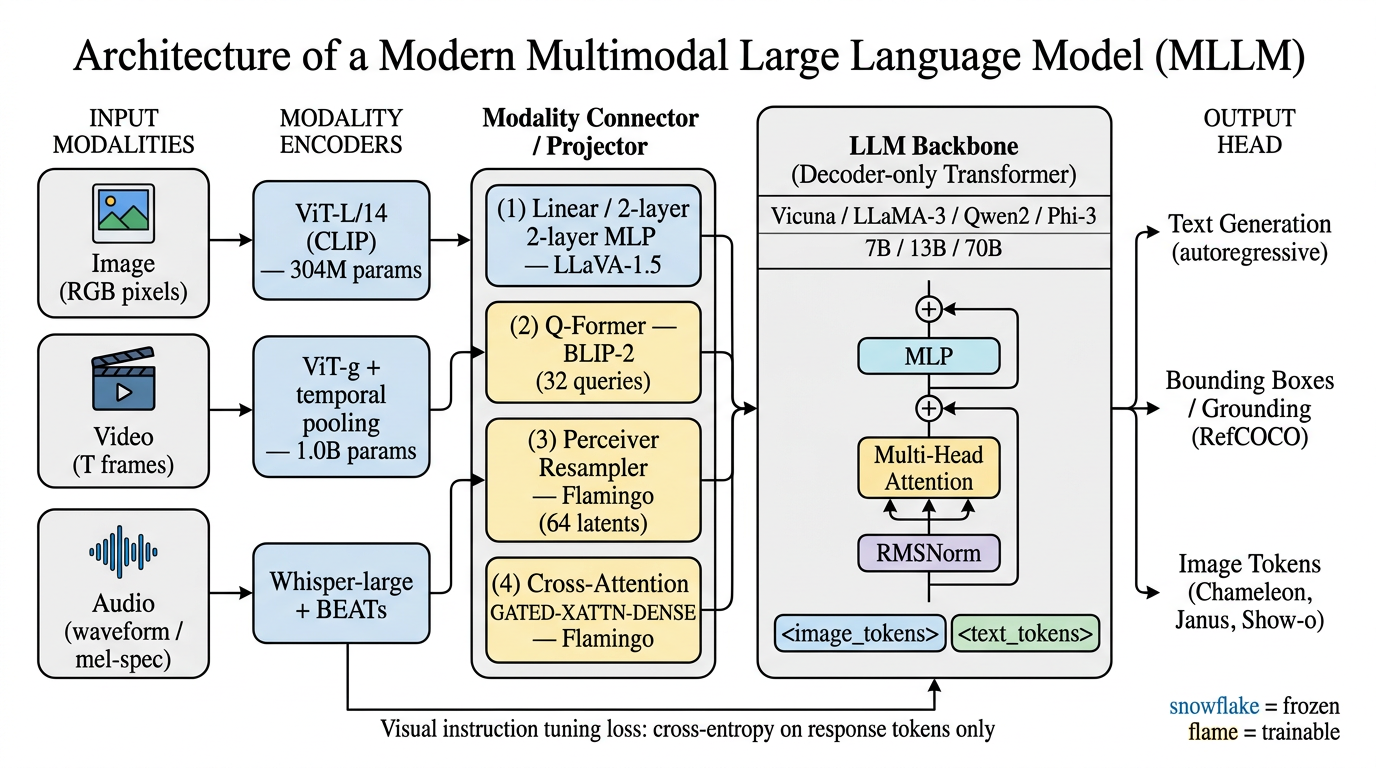
\includegraphics[width=\linewidth,keepaspectratio]{./figures/Multimodal-Large-Language-Models__fig1_mllm_architecture.png}}
\caption{Architecture of a modern Multimodal Large Language Model (MLLM): vision/audio/video encoders feed a modality connector --- linear MLP, Q-Former, or Perceiver Resampler --- that projects features into the token space of a decoder-only LLM backbone..}\label{fig:fig1-mllm-architecture}\end{figure}

\section{Executive Overview}\label{executive-overview}

Representative MLLM systems include: ViLBERT (2019, two-stream V+L Transformer with co-attention), CLIP (2021, web-scale image--text contrastive learning over 400M pairs), Flamingo (2022, frozen LLM with Perceiver Resampler and gated cross-attention), BLIP-2 (January 2023, Q-Former bridge to a frozen LLM), MiniGPT-4 (April 2023, single linear layer to Vicuna-13B with 3.5K curated pairs), LLaVA (April 2023, MLP projector with 158K GPT-4-generated instruction triples), InstructBLIP (May 2023, instruction-aware Q-Former across 13 datasets), Qwen-VL (August 2023, 256-query cross-attention with progressive resolution), GPT-4V (September 2023, first widely deployed frontier MLLM), Gemini 1.0 (December 2023, native interleaved text/image/audio/video pretraining), GPT-4o (May 2024, sub-300 ms voice and vision), Gemini 1.5 Pro (February 2024, 1M-token context for hour-long videos), InternVL-2.5-78B (December 2024, MMMU val 70.1 at 78B), Qwen2-VL-72B (September 2024, M-RoPE for 16,384 visual tokens), DeepSeek-VL2 (December 2024, 27B-active out of 236B MoE), Chameleon (May 2024, early-fusion VQ tokens with 8,192 codebook), Show-o (August 2024, autoregressive text plus discrete diffusion image tokens), Janus-Pro (January 2025, decoupled understanding and generation encoders at 7B), and Liquid (2024, single autoregressive Transformer over interleaved discrete tokens at 7B and 32B).

The taxonomy in Section 3 organises systems along five orthogonal axes. Axis one is the modality bridge: linear/MLP, Q-Former, Perceiver Resampler, cross-attention insertion, early-fusion VQ tokens, or MoE expansion. Axis two is modality coverage: image only, video, audio, document, 3D, or robotic action. Axis three is dense versus sparse parameterisation. Axis four separates frozen from trainable components. Axis five distinguishes understanding-only systems from any-to-any generative systems.

The training pipeline of Section 4 has converged on four stages. Stage one is vision encoder pretraining with CLIP- or SigLIP-style image--text contrastive (ITC) loss. Stage two is connector alignment on 0.5--1B image--caption pairs. Stage three is visual instruction tuning on 0.16--10M GPT-4-generated triples. Stage four is preference optimisation via factually augmented RLHF or Direct Preference Optimisation (DPO).

The benchmark landscape splits into four clusters. Perception suites cover MME (2,374 yes/no items), MMBench (3,217 MCQ), and SEED-Bench (19,242 MCQ). Knowledge and reasoning suites include MMMU (11.5K college-level questions across 30 subjects), MMMU-Pro, MathVista (6,141 problems), and BLINK (14 perception tasks). Hallucination suites include POPE, HallusionBench (1,129 trick questions), and MMHal-Bench. Modality-specific suites cover Video-MME for 30--60 min videos, AIR-Bench for audio, GMAI-MMBench's 26,675 medical samples, and Mind2Web and WebArena for GUI agents.

As of 2025, frontier closed models cluster at MMMU-val 62--70, MMBench-EN 80--87, MathVista 58--68, and POPE-F1 around 90--91. Open-source 70B-class models such as InternVL-2.5-78B and Qwen2-VL-72B match closed models on MMBench. They still trail by 5--10 points on MathVista and on long video. Four live limitations matter. First, visual jailbreak attacks succeed: Qi et al.~(2024) break MiniGPT-4, LLaVA, and InstructBLIP with imperceptible PGD perturbations. Second, object, attribute, and relation hallucination persists: POPE-adversarial F1 still sits near 86 for open 13B models. Third, benchmark contamination is widespread: Chen et al.~(2024) show many MMBench items are language-only solvable. Fourth, performance drops sharply on long videos beyond 30 minutes.

The survey closes in Section 11 with eight falsifiable predictions for 2026 to 2027. The predictions cover reasoning RL, unified generation, dynamic evaluation, energy disclosure, generalist VLAs, certified visual robustness, episodic memory, and edge MLLMs at 1B parameters.

The remainder of the paper is organised as follows. Section 1 defines MLLMs and lays out the token-mixing assumption that ties together LLaVA, Qwen-VL, and InternVL. Section 2 narrates the four historical eras and explains why each transition happened. Section 3 develops the architectural taxonomy. Section 4 details the four-stage training pipeline. Section 5 covers modality-specific MLLMs (video, audio, document, 3D, action). Section 6 catalogues the data ecosystem. Section 7 maps the benchmark landscape. Section 8 surveys deployed application domains. Section 9 enumerates failure modes and safety. Section 10 examines efficiency, compute, and edge deployment. Section 11 closes with predictions.

\section{Concepts, Notation, and the Anatomy of a Modern MLLM}\label{concepts-notation-and-the-anatomy-of-a-modern-mllm}

Building on the executive map above, this section pins down the formal definition, the notation, and the anatomical components that recur in every modern MLLM. We deliver three things: a working definition, the conditional probability formalism, and a short tour of cross-modal alignment, the modality gap, and emergent capabilities.

A \emph{Multimodal Large Language Model} (MLLM) is a single conditional language model. Its context window is extended, through learned interfaces, to ingest and sometimes emit information in modalities beyond text. The most common extra modality is image. Video, audio, point clouds, sensor traces, and robotic actions are increasingly supported. The defining structural property is one autoregressive decoder-only Transformer playing the role of a universal reasoner. Task-specific perception is delegated to upstream encoders whose outputs are projected into the LLM's token embedding space.

This commitment separates MLLMs from earlier vision-language pretraining (VLP) systems. Representative VLP systems include: ViLBERT (2019, co-attentional two-stream Transformer), LXMERT (2019, separate language and vision encoders with five pretraining objectives), VisualBERT (2019, single-stream merging of text and detected regions), VL-BERT (2020, Faster R-CNN regions plus BERT), OSCAR (2020, object tags as alignment anchors), VinVL (2021, improved object detector raising VQAv2 dev-test from 70.9 to 76.6), and ViLT (2021, patch-level fusion without object detection). These systems used two-stream Transformers without a strong language model behind them. They were fine-tuned per task rather than instruction-tuned for open-ended dialogue. The surveys of Yin et al.~(2023), Caffagni et al.~(2024), and Zhang et al.~(2024) reserve the abbreviation MLLM for systems built on top of a contemporary instruction-tuned LLM such as LLaMA, Vicuna, Qwen, Mistral, or GPT-4.

Formally, an MLLM defines a conditional distribution \(p_\theta(y_{1:T} \mid X_{1:M}, c)\) where \(X_{1:M} = (x^{(1)}, \ldots, x^{(M)})\) is a sequence of multimodal inputs (e.g., \(x^{(1)}\) is an image tensor, \(x^{(2)}\) is a text prompt, \(x^{(3)}\) is an audio clip), \(c\) is an optional system prompt or instruction, and \(y_{1:T}\) is the response token sequence. Training maximises the standard log-likelihood \(\sum_t \log p_\theta(y_t \mid y_{<t}, X_{1:M}, c)\), but supervision is typically applied only on the \emph{response} tokens, not on the visual or instruction tokens --- a design choice introduced by Visual Instruction Tuning \citep{liu2023visualinstructiont} and now near-universal. Each non-text input \(x^{(m)}\) is mapped through a learned encoder \(f^{(m)}_\phi\) to a feature tensor \(h^{(m)}\), then through a connector \(g^{(m)}_\psi\) to a sequence of \(k^{(m)}\) pseudo-tokens that share the LLM's embedding dimension. The full LLM input becomes the concatenation \([\text{BOS}, g^{(1)}(f^{(1)}(x^{(1)})), \ldots, g^{(M)}(f^{(M)}(x^{(M)})), e(\text{prompt}), \text{Assistant:}, \ldots]\), where \(e(\cdot)\) is the LLM's text token embedding. This token-mixing assumption --- that projected visual or audio features can occupy ``slots'' in the LLM's input the same way ordinary subword tokens do --- is the architectural invariant that ties together LLaVA, MiniGPT-4, Qwen-VL, InternVL, and DeepSeek-VL.

\subsection{What is an MLLM? Definitions and Boundary Cases}\label{what-is-an-mllm-definitions-and-boundary-cases}

This subsection identifies three discriminating properties that mark a system as an MLLM rather than a generic vision-language model (VLM). There is no single agreed boundary, but the literature converges on three signals. First, an MLLM uses a \emph{contemporary, instruction-tuned LLM} as its backbone --- Vicuna, LLaMA-2/3, Qwen, Mistral, or Phi --- rather than a vanilla BERT-style or GPT-2-style language head. Second, an MLLM exposes a \emph{natural-language interface}: the model accepts arbitrary instructions and emits free-form text. It does not use fixed-task heads such as classification softmax or detection regression. Third, an MLLM exhibits \emph{emergent compositionality}: zero-shot in-context learning, multi-turn dialogue, chain-of-thought reasoning over visual content, and tool-use grounded by perception \citep{wang20242024}.

Under these criteria, BLIP-2 sits on the boundary because it uses an LLM but is not instruction-tuned out of the box. LLaVA, MiniGPT-4, InstructBLIP, and Flamingo are all squarely inside the MLLM category. CLIP and ALIGN, despite being foundational, are not MLLMs. They have no autoregressive language head: they produce embeddings, not generations.

A second taxonomic boundary concerns \emph{generation breadth}. Most early MLLMs were \emph{understanding-only} --- they accept images and emit text. Unified models such as Chameleon (Shi et al., 2024), Show-o \citep{xie20242024}, Janus and Janus-Pro \citep{wu20242024}, and Liquid \citep{wu20242024} extend the LLM's vocabulary with discrete image tokens and can generate pixels back, yielding an \emph{any-to-any} MLLM. NExT-GPT \citep{wu20242024} and AnyGPT push this further by interleaving audio, video, and image tokens. The cost is that early-fusion mixed-token models tend to underperform best-of-class understanding-only models on image-only benchmarks, an empirical gap quantified in the survey of Zhao et al.~(2025) on unified U+G models.

\subsection{Cross-Modal Alignment, Modality Gap, and Token Interfaces}\label{cross-modal-alignment-modality-gap-and-token-interfaces}

This subsection reviews the four token-interface families that bridge sensor outputs and LLM input. The central mechanical question of MLLM design is how to convert continuous, high-dimensional sensor outputs into a token sequence that an LLM can attend to. Four widely used solutions dominate the design space. The simplest is the \emph{linear or MLP projector} used by LLaVA: a 1- or 2-layer feedforward network maps the 1024- or 1408-dimensional ViT patch embeddings into the LLM's hidden size --- 4096 for LLaMA-2-7B, 8192 for LLaMA-3-70B --- so each ViT patch becomes one LLM token and the visual-token count equals the patch count (576 for ViT-L/14 at 336²). The \emph{Q-Former} of BLIP-2 \citep{li2023blip2bootstrapping} distils the ViT features into a fixed pool of 32 learned query tokens through a 12-layer cross-attention Transformer, trained in two stages with Image-Text Contrastive (ITC), Image-Text Matching (ITM), and Image-grounded Text Generation (ITG) losses. The \emph{Perceiver Resampler} of Flamingo \citep{alayrac20222022} uses 64 learnable latents that cross-attend to image features and are injected into the frozen LLM via GATED-XATTN-DENSE layers initialised at zero, preserving the original LLM behaviour at the start of training. The \emph{cross-attention insertion} variant inserts new attention layers within the LLM rather than appending tokens upstream. Recent unified models replace the projector entirely with a \emph{VQ tokenizer}: Chameleon uses 8,192-codebook image tokens, while Janus adopts a separate understanding encoder distinct from the generation encoder.

Across all of these designs, an empirical phenomenon called the \emph{modality gap} has been documented: when image and text embeddings produced by CLIP-style contrastive training are visualised in ℝ⁵¹², they occupy disjoint cones rather than the same subspace, even when they should be semantically aligned. This gap also appears inside MLLMs, where visual tokens cluster separately from text tokens in early LLM layers and only mix in the upper third \citep{bordes20242024}. The practical consequence is that MLLMs need either large amounts of paired alignment data (LLaVA: 558K LAION-CC-SBU captions in stage one) or carefully designed bridges (Q-Former) to overcome the gap.

\subsection{Emergent Capabilities Distinguishing MLLMs from VLP Predecessors}\label{emergent-capabilities-distinguishing-mllms-from-vlp-predecessors}

This subsection lists the three emergent behaviours that mark the qualitative gap between MLLMs and pre-2022 VLP encoders. Three families of emergent capabilities are reproducibly observed across MLLMs and were never reliably exhibited by older VLP encoders. The first is \emph{open-ended visual instruction following}: a single LLaVA-1.5 checkpoint can describe an X-ray, parse a receipt, write code from a wireframe, and continue a chat without any task-specific head. The second is \emph{visual chain-of-thought}: models such as InternVL-2.5, Qwen2-VL, and Gemini 1.5 Pro respond to ``let's think step by step'' over a chart or geometry figure with intermediate reasoning that demonstrably improves answer accuracy on MathVista by +8--14 absolute points \citep{lu20242024}. The third is \emph{tool-grounded perception}: GPT-4V and Gemini can invoke external tools --- web search, code interpreter, retrieval --- based on what they see, a capability that drives downstream agent applications such as SeeAct \citep{zheng20242024} and CogAgent for GUI control. These three behaviours motivate the rest of the survey: every subsequent design choice --- visual token compression, RLHF, hallucination mitigation, MoE routing --- exists ultimately to make them more reliable, more efficient, and more deployable.

\begin{table*}[t]
\centering
\caption{Emergent Capabilities Distinguishing MLLMs from VLP Predecessors: Term, Meaning in this survey.}
\label{tab:emergent-capabilities-distinguishing-mllms-from-vlp-predeces}
\begin{tabular}{>{\raggedright\arraybackslash}p{0.2451\linewidth}
  >{\raggedright\arraybackslash}p{0.7549\linewidth}}
\toprule
\textbf{Term} & \textbf{Meaning in this survey} \\
\midrule
MLLM & LLM extended with non-text encoders/decoders sharing a common token interface \\
LVLM & Large Vision-Language Model --- synonym for image-text MLLM in the literature \\
VLP & Vision-Language Pretraining (the pre-2021 encoder-only era) \\
Q-Former & Querying Transformer of BLIP-2 with 32 learnable tokens \\
Resampler & Perceiver-style module of Flamingo with 64 latents \\
Visual instruction tuning & Supervised fine-tuning on (image, instruction, response) triples \\
Modality connector & Trainable module mapping visual/audio features into LLM hidden dim \\
ITC / ITM / ITG & Image-Text Contrastive / Matching / Generation losses \\
Hallucination & Generated content not supported by the visual input \\
VLA & Vision-Language-Action model (RT-2, OpenVLA) \\
\end{tabular}
\end{table*}

This survey takes the position that MLLMs are best understood as the natural extension of LLMs once a modality interface and a sufficiently rich instruction corpus exist; everything else --- taxonomies, benchmarks, applications, failure modes, predictions --- follows from that single architectural commitment. The remaining sections develop the view systematically: Section 2 traces the historical trajectory from ViLBERT in 2019 to GPT-4o, Gemini 2, and Janus-Pro in 2025--2026; Section 3 lays out the architectural taxonomy with concrete model families; Section 4 details the four-stage training pipeline; Sections 5 and 6 cover modality-specific MLLMs and the data ecosystem; Section 7 surveys the benchmark landscape; Section 8 enumerates application domains; Section 9 examines failure modes and safety; Section 10 covers efficiency; and Section 11 closes with falsifiable predictions for 2026--2027.

\section{Historical Trajectory: From Two-Stream V+L Transformers to GPT-4o}\label{historical-trajectory-from-two-stream-vl-transformers-to-gpt-4o}

\begin{figure}[t]
\centering
\pandocbounded{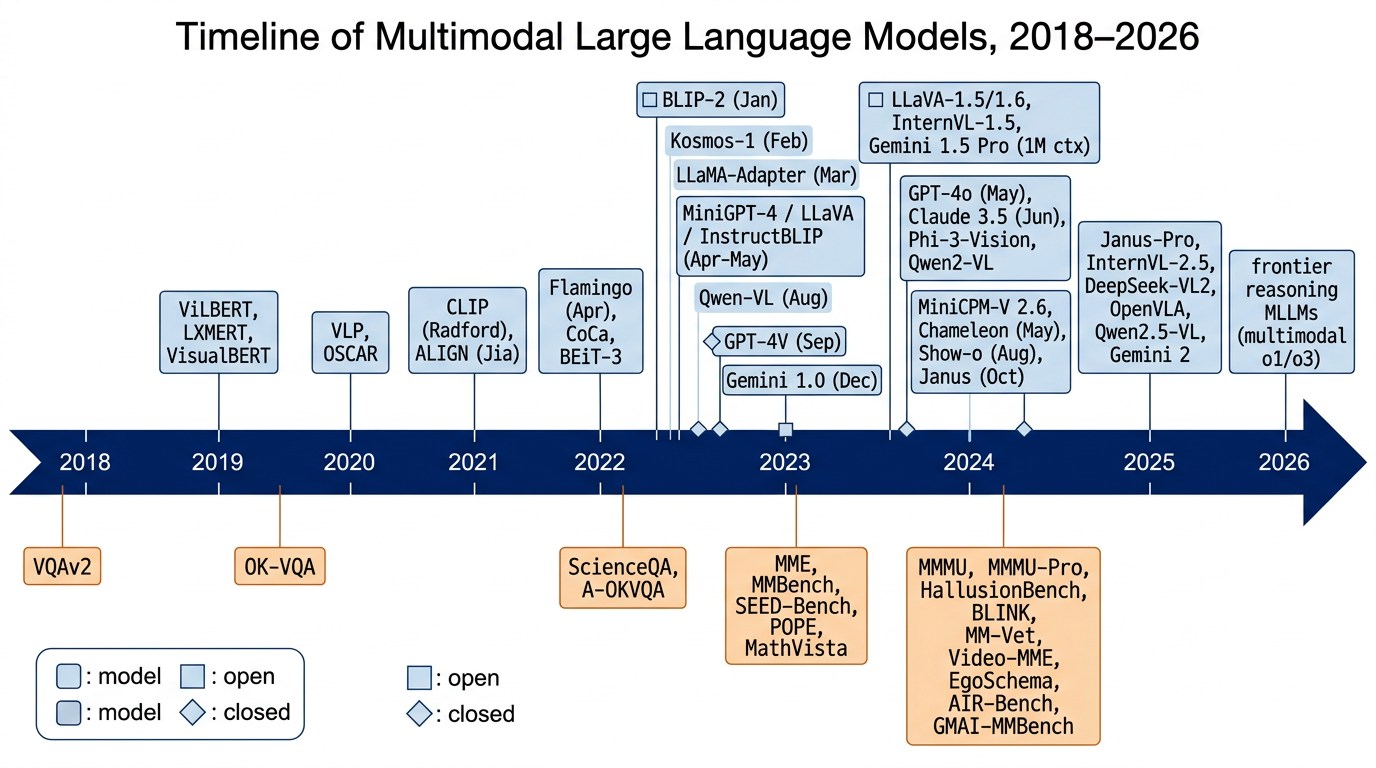
\includegraphics[width=\linewidth,keepaspectratio]{./figures/Multimodal-Large-Language-Models__fig5_timeline.png}}
\caption{Timeline of Multimodal Large Language Models, 2018--2026: from two-stream V+L Transformers (ViLBERT, LXMERT, VisualBERT) through CLIP-era contrastive pretraining and the 2023 visual-instruction-tuning inflection (BLIP-2, LLaVA, MiniGPT-4, Instruct.}\label{fig:fig5-timeline}\end{figure}

Whereas Section 1 fixed the formal definition and the token-interface mechanics, this section turns to the historical pathway that produced today's MLLMs. This section reviews four eras of multimodal language modelling, organised by the supervision signal that defined each era.

The history of multimodal language modelling can be partitioned into four eras. Each era is defined by a different answer to the question ``what does cross-modal supervision look like?''. Era one is object-region masked language modelling (2018--2021). Era two is web-scale contrastive InfoNCE (2021--2022). Era three is LLM-bridge visual instruction tuning (2022--early 2024). Era four is natively multimodal pretraining with unified understanding-and-generation (2024--2026). Concrete inflection points anchor each transition: VinVL's VQAv2 jump from 70.9 to 76.6 in 2021 closed the encoder-only era; CLIP ViT-L/14 reaching 76.2\% zero-shot ImageNet top-1 in 2021 launched the contrastive era; LLaVA's release on April 17 2023 (alongside MiniGPT-4 the same week) launched visual instruction tuning; GPT-4V's September 2023 deployment and Gemini 1.0 Ultra's December 2023 launch with 59.4\% MMMU val opened the natively multimodal frontier. Architectural choices, training corpora, and evaluation conventions in 2026 still inherit biases from each era --- encoder choice from CLIP, instruction recipes from LLaVA, generation tokens from Chameleon. Table 2 summarises the chronology before we expand on the transitions.

\begin{table*}[t]
\centering
\caption{Historical Trajectory: From Two-Stream V+L Transformers to GPT-4o: Era, Years, Representative systems, Defining property.}
\label{tab:historical-trajectory-from-two-stream-v-l-transformers-to-gp}
\begin{tabular}{>{\raggedright\arraybackslash}p{0.1467\linewidth}
  >{\raggedright\arraybackslash}p{0.0667\linewidth}
  >{\raggedright\arraybackslash}p{0.4222\linewidth}
  >{\raggedright\arraybackslash}p{0.3644\linewidth}}
\toprule
\textbf{Era} & \textbf{Years} & \textbf{Representative systems} & \textbf{Defining property} \\
\midrule
Encoder-only V+L pretraining & 2018--2021 & ViLBERT, LXMERT, VisualBERT, VL-BERT, OSCAR, VinVL, ViLT & Two-stream Transformers, masked-language + image-text matching, fine-tune per task \\
Web-scale contrastive & 2021--2022 & CLIP, ALIGN, BASIC, CoCa, BEiT-3 & InfoNCE on hundreds of millions of noisy image-text pairs; zero-shot transfer \\
LLM-bridge \& instruction tuning & 2022--early 2024 & Flamingo, BLIP-2, Kosmos-1, LLaMA-Adapter, MiniGPT-4, LLaVA, InstructBLIP, Qwen-VL, IDEFICS & LLM as the brain; lightweight bridge; visual instruction tuning \\
Frontier multimodal \& unified U+G & 2024--2026 & GPT-4V/4o, Gemini 1.5/2, Claude 3.5, InternVL-2.5, Qwen2-VL, Chameleon, Show-o, Janus-Pro, RT-2 & Native multimodal pretraining; long context; unified understanding+generation \\
\end{tabular}
\end{table*}

\subsection{The Encoder-Only V+L Era (2018--2021): ViLBERT, LXMERT, VisualBERT}\label{the-encoder-only-vl-era-20182021-vilbert-lxmert-visualbert}

This subsection summarises the encoder-only era and the structural limits that motivated the next era. Representative methods include: ViLBERT (2019, co-attentional Transformer with two streams that exchange keys and values), LXMERT (2019, separate language and vision encoders with five pretraining objectives), VisualBERT (2019, single-stream merge of text and detected regions), VL-BERT (2020, unified Transformer over Faster R-CNN regions and tokens), UNITER (2020, masked region modelling with conditional masking), OSCAR (2020, object tags as anchors raising VQAv2 to 73.6), VinVL (2021, improved object detector raising VQAv2 dev-test from 70.9 to 76.6), and ViLT (2021, patch-level fusion that drops object detection).

Modern MLLMs descend, conceptually, from two-stream Transformers that learned cross-modal representations using BERT-style masked objectives over text paired with detected object regions (Faster R-CNN features). LXMERT \citep{tan2019lxmertlearningcros} introduced separate language and vision encoders connected by a cross-modality encoder, trained with five objectives --- masked LM, masked object prediction (label and feature regression), cross-modality matching, and image-question answering on 9.18M image-sentence pairs from MS-COCO, Visual Genome, VQAv2, GQA, and VG-QA. ViLBERT \citep{lu2019vilbertpretraining} used a co-attentional Transformer with two streams that exchanged keys and values, pretraining on 3.3M Conceptual Captions pairs. VisualBERT and VL-BERT (2019--2020) merged the two streams into a single Transformer. OSCAR (Li et al., 2020) and VinVL (2021) added object tags as anchors, raising VQAv2 dev-test from 70.9 to 76.6. Despite strong fine-tuning numbers, these models had three structural limitations that motivated the next era: (1) they relied on object detector features and inherited their failure modes; (2) they were never instruction-tuned and could not chat; (3) they pretrained on a few million captions rather than the billions that would soon become available. In retrospect, the encoder-only V+L era proved that joint Transformer modelling of vision and language was feasible, but it was the wrong unit --- it produced classifiers, not assistants.

\subsection{Contrastive Foundations: CLIP, ALIGN, CoCa, and Web-Scale Image-Text Pretraining}\label{contrastive-foundations-clip-align-coca-and-web-scale-image-text-pretraining}

This subsection traces the contrastive era and the lasting contribution it made to every subsequent MLLM: a strong vision tower. Representative contrastive systems include: CLIP (2021, symmetric InfoNCE on 400M image--text pairs reaching 76.2\% zero-shot ImageNet top-1), ALIGN (2021, scaling the recipe to 1.8B noisy pairs), BASIC (2022, 6.6B-parameter joint scaling of model and data), FLIP (2023, fast language--image pretraining via patch masking), CoCa (2022, contrastive captioner adding a language head and an attentional pooler), BEiT-3 (2022, masked-data modelling with multiway Transformers), SigLIP (2023, replacing softmax InfoNCE with sigmoid loss for batch-independent training), EVA-CLIP (2023, scaling vision Transformers with masked image modelling pretraining), DINOv2 (2023, self-supervised features on 142M curated images), and InternViT-6B (2024, 6B-parameter vision tower distilled from 1.5B images).

The 2021 papers CLIP (Radford et al.) and ALIGN (Jia et al.) reframed cross-modal learning as a \emph{retrieval} problem: given an image and a caption from a web-scraped pool of 400M (CLIP) or 1.8B (ALIGN) pairs, maximise their cosine similarity in a shared embedding space using the symmetric InfoNCE loss
\[\mathcal{L}_{\text{ITC}} = -\frac{1}{2N}\sum_i \left[\log\frac{\exp(\langle v_i, t_i\rangle / \tau)}{\sum_j \exp(\langle v_i, t_j\rangle/\tau)} + \log\frac{\exp(\langle v_i, t_i\rangle/\tau)}{\sum_j \exp(\langle v_j, t_i\rangle/\tau)}\right].\]
This produced visual features that transferred zero-shot to ImageNet (CLIP ViT-L/14 at 336² reaches 76.2\% top-1) and to dozens of classification benchmarks. CoCa \citep{yu20222022} added a captioning head and an attentional pooler, establishing the template that later MLLMs would generalise. BASIC, FLIP, and SigLIP refined the loss. CLIP and ALIGN are not MLLMs themselves --- they have no autoregressive language head --- but their \emph{visual encoders} became the de facto perception front-end for nearly every subsequent MLLM: LLaVA, MiniGPT-4, InstructBLIP, BLIP-2, Qwen-VL, and InternVL all use CLIP-style ViT-L/14 or ViT-g/14 as their image encoder. The contrastive era thus contributed the vision tower; the LLM era would contribute the brain.

\subsection{The Inflection Point of 2023: BLIP-2, LLaVA, MiniGPT-4, InstructBLIP}\label{the-inflection-point-of-2023-blip-2-llava-minigpt-4-instructblip}

This subsection narrates the six-month window in 2023 that produced the modern visual-instruction-tuning template. Representative inflection-point systems include: BLIP-2 (January 2023, Q-Former bridging frozen ViT-g and frozen Flan-T5 with 188M trainable parameters), Kosmos-1 (February 2023, 1.6B-parameter Transformer trained from scratch on interleaved image--text), LLaMA-Adapter (March 2023, zero-init attention with 1.2M trainable parameters), LLaMA-Adapter V2 (April 2023, vision branch via CLIP soft prompts), MiniGPT-4 (April 17 2023, BLIP-2 Q-Former plus a single linear layer to Vicuna-13B), LLaVA (April 17 2023, MLP projector plus 158K GPT-4-generated visual instructions), InstructBLIP (May 2023, instruction-aware Q-Former across 13 datasets), Otter (June 2023, OpenFlamingo with MIMIC-IT instruction tuning), Qwen-VL (August 2023, 256-query cross-attention plus 224²→448² progressive training), mPLUG-Owl (April 2023, modularised LLaVA-style training), and IDEFICS-1 (August 2023, public 9B/80B Flamingo replication on OBELICS).

The transition to the modern MLLM happened in a six-month window between January and June 2023. \textbf{BLIP-2} \citep{li2023blip2bootstrapping} introduced the Q-Former and froze both ViT-g and a Flan-T5 or OPT LLM, training only 188M parameters in the bridge. With FlanT5-XXL it achieved zero-shot VQAv2 65.0 and GQA 44.7 --- competitive with end-to-end fine-tuned models 30× larger. \textbf{Kosmos-1} \citep{huang20232023} trained a 1.6B-param Transformer from scratch on interleaved image-text data and demonstrated multimodal in-context learning. \textbf{LLaMA-Adapter} \citep{zhang2023videollamaaninstru} and \textbf{LLaMA-Adapter V2} \citep{gao20232023} introduced zero-init attention to make instruction tuning of LLaMA cheap (1.2M trainable params). \textbf{MiniGPT-4} \citep{zhu2024minigpt4enhancingv} connected BLIP-2's Q-Former to Vicuna-13B with a single linear layer and exposed the GPT-4-like behaviour of describing images and generating websites from sketches. \textbf{LLaVA} \citep{liu2023visualinstructiont} made the simplest move of all --- a linear projector connecting CLIP-ViT-L/14 to Vicuna --- but introduced visual instruction tuning with 158K GPT-4-generated multimodal instructions, which is what gave the system its conversational fluency. \textbf{InstructBLIP} \citep{dai20232023} systematised instruction-aware Q-Former training over 13 datasets. By the summer, Qwen-VL \citep{bai20232023}, mPLUG-Owl, and IDEFICS (HuggingFace's Flamingo replication) had appeared. The resulting recipe --- frozen vision tower, lightweight connector, instruction-tuned LLM, GPT-4-generated dialogue data --- became the dominant template.

\subsection{Frontier Closed and Open Models (2024--2026)}\label{frontier-closed-and-open-models-20242026}

This subsection covers the 2024--2026 frontier and the bifurcation between understanding-only systems and unified understanding-and-generation systems. Representative frontier systems include: GPT-4V (September 2023, first widely deployed frontier vision--language API), Gemini 1.0 Ultra (December 2023, native interleaved text/image/audio/video reaching 59.4 MMMU val), GPT-4o (May 2024, sub-300 ms unified text--image--audio I/O), Gemini 1.5 Pro (February 2024, 1M-token context for hour-long videos), Claude 3.5 Sonnet (June 2024, closing much of the open-source gap on perception), InternVL-1.5 (April 2024, dynamic resolution up to 4K×4K), InternVL-2.5-78B (December 2024, MMMU val 70.1 and BLINK 60.0), Qwen2-VL-72B (September 2024, M-RoPE for 16,384 visual tokens), DeepSeek-VL2 (December 2024, 27B-active out of 236B MoE), MiniCPM-V 2.6 (2024, GPT-4V-level capability at 8B running on iPhone), Phi-3-Vision (April 2024, 4.2B edge model), Mini-InternVL (2024, 2B compact MLLM), Chameleon (May 2024, mixed-modal early-fusion Transformer at 7B and 30B), Show-o (August 2024, autoregressive text plus discrete diffusion images at 1.3B), Janus (October 2024, decoupled understanding and generation encoders sharing one LLM), Janus-Pro-7B (January 2025, MMMU 41.0 and GenEval 0.80), Liquid (2024, single autoregressive Transformer at 7B and 32B over interleaved discrete tokens), RT-2 (2023, vision--language--action with semantic generalisation), and Gemini Robotics (2025, first commercial frontier VLA).

In September 2023 OpenAI released \textbf{GPT-4V} publicly, and in December 2023 Google released \textbf{Gemini 1.0} (Ultra, Pro, Nano) (Gemini Team, 2023), the first frontier model trained natively on interleaved text, image, audio, and video tokens --- Gemini 1.0 Ultra reached 59.4\% on MMMU val and 47.9 on MMMU MathVista combined evaluation. May 2024 brought \textbf{GPT-4o}, the first commercial model with native unified input/output across text, image, and audio, with claimed sub-300 ms voice latency. \textbf{Gemini 1.5 Pro} (February 2024) extended the context window to 1M tokens, enabling reasoning over hour-long videos. \textbf{Claude 3.5 Sonnet} (June 2024) closed much of the open-source gap. On the open side, \textbf{InternVL-1.5} \citep{chen20242024} introduced dynamic high-resolution input up to 4K×4K, \textbf{InternVL-2.5-78B} (December 2024) reached MMMU 70.1, and \textbf{Qwen2-VL-72B} (Sept 2024) supported up to 16,384 dynamic visual tokens with multimodal RoPE. \textbf{MiniCPM-V 2.6} \citep{yao20242024} demonstrated GPT-4V-level capability at 8B parameters running on consumer phones. \textbf{Phi-3-Vision} (Microsoft, April 2024, 4.2B params) and \textbf{Mini-InternVL} (2B) confirmed that pocket MLLMs were viable.

In parallel, \emph{unified understanding-and-generation} models redefined the architectural ceiling. \textbf{Chameleon} (Meta, May 2024) trained a mixed-modal early-fusion Transformer on 4.4T tokens with discrete VQ image tokens and a unified vocabulary of 65K text + 8192 image tokens. \textbf{Show-o} \citep{xie20242024} combined autoregressive text with discrete diffusion for image tokens in one model. \textbf{Janus} and \textbf{Janus-Pro} \citep{wu20242024} decoupled the visual encoder for understanding from the generator for synthesis but kept a single LLM. \textbf{Liquid} \citep{wu20242024} used a single autoregressive Transformer over interleaved discrete image+text tokens to scale unified U+G to 7B and 32B params. By 2025--2026 the frontier had bifurcated: (1) reasoning-heavy MLLMs adopting o1-style chain-of-thought RL --- multimodal o1, Gemini 2 with Deep Think; (2) embodied \textbf{VLA} models --- RT-2, RT-X (Open X-Embodiment, 1.4M episodes across 22 robots), OpenVLA (7B), Gemini Robotics --- bringing MLLM reasoning to real-world action.

\begin{table*}[t]
\centering
\caption{Frontier Closed and Open Models (2024--2026): Year, Open-source leader, Closed-source leader, Defining release.}
\label{tab:frontier-closed-and-open-models-2024-2026}
\begin{tabular}{>{\raggedright\arraybackslash}p{0.0727\linewidth}
  >{\raggedright\arraybackslash}p{0.3818\linewidth}
  >{\raggedright\arraybackslash}p{0.2545\linewidth}
  >{\raggedright\arraybackslash}p{0.2909\linewidth}}
\toprule
\textbf{Year} & \textbf{Open-source leader} & \textbf{Closed-source leader} & \textbf{Defining release} \\
\midrule
2021 & CLIP & -- & Web-scale image-text contrastive \\
2022 & OpenFlamingo (later) & -- & Flamingo cross-attention bridge \\
2023 & LLaVA / InstructBLIP & GPT-4V (Sep) & Visual instruction tuning \\
2024 & InternVL-1.5 / Qwen2-VL & GPT-4o, Gemini 1.5 & Native multimodal + 1M context \\
2025 & InternVL-2.5 / Janus-Pro / DeepSeek-VL2 & GPT-4o, Gemini 2, Claude 3.5 & Unified U+G, MoE \\
2026 & OpenVLA / Qwen2.5-VL / multimodal-o3-style & frontier reasoning MLLMs & VLA + perceptual reasoning RL \\
\end{tabular}
\end{table*}

Several lessons from this trajectory shape the rest of the survey. First, \emph{data quality dominates raw quantity once instruction tuning enters the picture}: ShareGPT4V's 1.2M GPT-4V-recaptioned pairs \citep{chen20242024} outperformed raw LAION-2B on perception benchmarks. Second, \emph{open-source narrowed the understanding gap but not the reasoning gap} --- InternVL-2.5-78B matches GPT-4o on MMMU (≈70\%) but trails on MathVista, BLINK, and especially on long video. Third, \emph{unified generation is technically feasible but performance-trading}: Janus-Pro-7B reaches GenEval 0.80 (above SDXL) but trails LLaVA-1.5 by 1--3 points on MMBench. Fourth, the \emph{safety/alignment frontier} has decisively moved to multimodal: visual jailbreak \citep{qi20242024}, image-conditioned prompt injection, and RAG poisoning are now first-class concerns. These threads, all visible in the timeline, are developed in Sections 3 (architectures), 4 (training), 9 (safety), and 10 (efficiency).

\subsection{Why each transition happened}\label{why-each-transition-happened}

The encoder-only V+L era ended when CLIP showed that web-scale paired data with a simple symmetric loss outperforms hand-crafted multi-task pretraining. The contrastive era ended when researchers realised that embeddings without a generative head cannot follow instructions or reason. The bridge era of 2023 ended once frontier proprietary models such as GPT-4V demonstrated capability ceilings that small bridges with frozen LLMs cannot match without scaling everything --- vision tower, connector, LLM, and data --- together. The transition into the unified-generation era is now under way, driven by the goal of one model that can both perceive and produce, the missing half of artificial general intelligence as articulated by Liang, Zadeh, and Morency (2024) in their Foundations and Trends review. Whether this push will succeed, and at what cost, is the subject of Section 11. We turn next to the architectural taxonomy that organises the systems produced by these four eras.

\section{Taxonomy of MLLM Architectures}\label{taxonomy-of-mllm-architectures}

\begin{figure}[t]
\centering
\pandocbounded{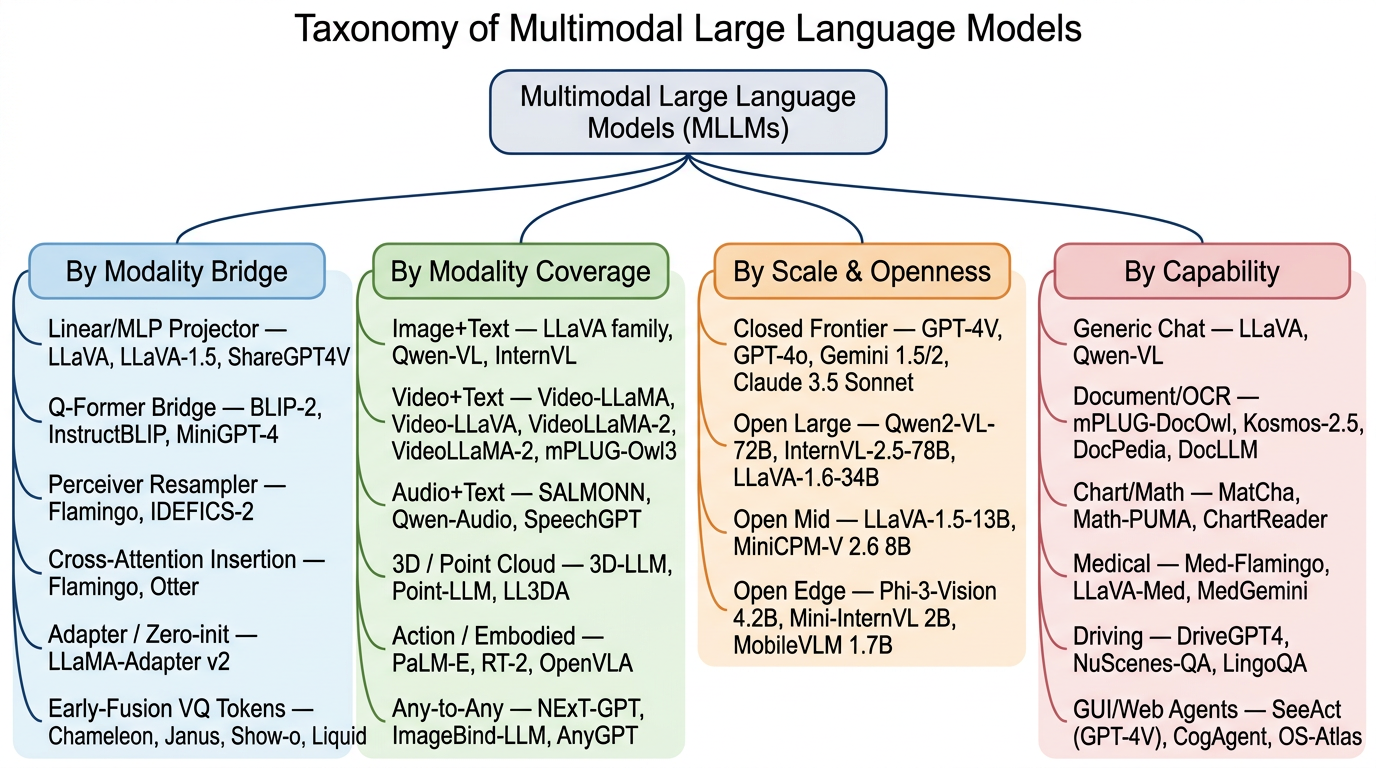
\includegraphics[width=\linewidth,keepaspectratio]{./figures/Multimodal-Large-Language-Models__fig2_taxonomy_tree.png}}
\caption{Taxonomy of Multimodal Large Language Models --- by modality bridge, modality coverage, scale/openness, and capability --- with concrete model exemplars under each leaf.}\label{fig:fig2-taxonomy-tree}\end{figure}

Building on the historical trajectory in Section 2, this section organises the resulting design space into a single taxonomy. This section reviews five orthogonal architectural axes --- modality bridge, modality coverage, parameterisation, frozen-versus-trainable components, and understanding-versus-generation scope --- and instantiates each axis with concrete model families.

Architectural choices in MLLMs cluster along five largely orthogonal axes: which connector sits between encoder and LLM (linear/MLP, Q-Former, Perceiver Resampler, cross-attention, VQ tokens, MoE), which modalities are accepted (image, video, audio, 3D, action), how the LLM is parameterised (dense 7B--80B vs sparse MoE 27B-active out of 236B), what is frozen versus trainable (LLaVA trains the LLM; Flamingo and BLIP-2 freeze it), and whether the model can also generate non-text outputs (understanding-only vs unified U+G). Concrete exemplars span the design space: LLaVA-1.5 with a 2-layer MLP and 576 visual tokens at 336², Qwen-VL with 256 cross-attention queries at 448², BLIP-2 with a 32-token Q-Former, Flamingo's 64-latent Perceiver Resampler injected via GATED-XATTN-DENSE blocks, Chameleon's 8,192-codebook VQ tokens, and DeepSeek-VL2's 27B-active MoE. Within a single bridge family, MMBench-EN at the 7B scale typically spreads only 3--5 absolute points across well-trained variants, while crossing families changes the score by 8--15 points (Liu et al., 2024 MMBench paper). Bridge choice therefore determines the capability ceiling; everything downstream sets how close the model approaches that ceiling. Table 3 gives the method-family comparison; the subsections that follow expand each class with the parameter counts, token budgets, and ablation deltas needed to compare them rigorously.

\begin{table*}[t]
\centering
\caption{Taxonomy of MLLM Architectures: Bridge family, Representative MLLMs, \# vis. tokens, Trainable in stage 1.}
\label{tab:taxonomy-of-mllm-architectures}
\begin{tabular}{>{\raggedright\arraybackslash}p{0.1624\linewidth}
  >{\raggedright\arraybackslash}p{0.2487\linewidth}
  >{\raggedright\arraybackslash}p{0.0863\linewidth}
  >{\raggedright\arraybackslash}p{0.1218\linewidth}
  >{\raggedright\arraybackslash}p{0.1878\linewidth}
  >{\raggedright\arraybackslash}p{0.1929\linewidth}}
\toprule
\textbf{Bridge family} & \textbf{Representative MLLMs} & \textbf{\# vis. tokens} & \textbf{Trainable in stage 1} & \textbf{Strengths} & \textbf{Weaknesses} \\
\midrule
Linear / MLP projector & LLaVA, LLaVA-1.5, ShareGPT4V, Yi-VL & 576 (336²) & projector only (≈6M) & Simplicity, strong scaling & Token cost grows with resolution \\
Q-Former & BLIP-2, InstructBLIP, MiniGPT-4, X-LLM & 32 queries & Q-Former 188M & Compact context, two-stage curriculum & Information bottleneck on dense scenes \\
Perceiver Resampler + cross-attn & Flamingo, OpenFlamingo, IDEFICS-1/2, Otter & 64 latents & Resampler + XATTN & Few-shot in-context strong & Heavy LLM modification \\
Adapter / zero-init attention & LLaMA-Adapter v1/v2, BLIVA, Bunny & 0 (cross-attn) & adapters (1.2M--14M) & Parameter-efficient & Lower ceiling than full IT \\
Early-fusion VQ tokens & Chameleon, Show-o, Janus, Janus-Pro, Liquid, Emu2 & 1024--4096 VQ & full LLM & Unified U+G & Trades understanding for generation \\
MoE expansion & DeepSeek-VL2, MoE-LLaVA, MiniCPM-MoE & varies & sparse experts & Capacity at fixed compute & Routing complexity \\
\end{tabular}
\end{table*}

\subsection{Adapter / Projector Bridge (LLaVA Family, Qwen-VL, InternVL)}\label{adapter-projector-bridge-llava-family-qwen-vl-internvl}

This subsection surveys projector-bridge MLLMs, the now-dominant family. Representative projector-bridge systems include: LLaVA (April 2023, single linear layer from CLIP-ViT-L/14 to Vicuna), LLaVA-1.5 (October 2023, 2-layer MLP yielding +5.4 MMBench over linear), LLaVA-1.6/NeXT (January 2024, dynamic-resolution AnyRes for high-resolution OCR), ShareGPT4V (2024, MLP plus 1.2M GPT-4V recaptions), Yi-VL (2024, 2-layer MLP on Yi-34B/6B with bilingual support), Qwen-VL (August 2023, 256-query cross-attention with progressive 224²→448² training), Qwen2-VL (September 2024, M-RoPE plus dynamic visual tokens up to 16,384), InternVL-1.5 (April 2024, InternViT-6B plus Pixel Shuffle 2× plus 2-layer MLP at 4K resolution), InternVL-2.5-78B (December 2024, MMMU 70.1 and ChartQA 88.6), DeepSeek-VL (2024, hybrid SAM-B + SigLIP-L tower with MLP adapter), and Cambrian-1-34B (2024, vision-centric design with spatial-vision-aggregator).

The simplest and now most popular bridge is a small feedforward projector. \textbf{LLaVA} uses a single linear layer mapping ViT-L/14's 1024-dim patch embeddings to LLaMA's 4096-dim token space; \textbf{LLaVA-1.5} \citep{liu2024improvedbaselinesw} replaces the linear with a 2-layer MLP and reports a +1.7 absolute gain on VQAv2 and a +5.4 on MMBench from this single change. \textbf{Qwen-VL} \citep{bai20232023} uses a single cross-attention layer with 256 learnable queries and adds a 224×224 → 448×448 progressive training stage, reaching TextVQA 63.8 and DocVQA 65.1, the SOTA at its release. \textbf{InternVL-1.5} scales the \emph{vision tower} itself to 6B parameters (InternViT-6B distilled from 1.5B images) and uses a Pixel Shuffle 2× downsampler followed by a 2-layer MLP, sustaining dynamic-resolution input up to 4K×4K. \textbf{InternVL-2.5-78B} retains the same connector but pairs it with a 70B LLM and reaches MMMU val 70.1, BLINK 60.0, ChartQA 88.6 --- within 1.0 point of GPT-4o on most benchmarks. \textbf{DeepSeek-VL} uses a hybrid SAM-B + SigLIP-L vision tower with an MLP adapter and reports 56.6 MMBench-EN at the 7B scale.

The strength of the projector design is that it preserves the LLM unchanged, allowing weight reuse and easy back-porting of LLM-side improvements (instruction tuning, RLHF, longer context). Its weakness is that the number of visual tokens grows linearly with image area; LLaVA-1.5 emits 576 tokens at 336², and dynamic-resolution variants such as LLaVA-NeXT and Qwen2-VL can emit 4K--16K tokens, pressuring the LLM context window and dominating inference cost.

\subsection{Q-Former and Resampler Bridges (BLIP-2, InstructBLIP, Flamingo)}\label{q-former-and-resampler-bridges-blip-2-instructblip-flamingo}

This subsection covers the bridge family that compresses visual features to a fixed token budget. Representative compression-bridge systems include: BLIP-2 (January 2023, 32-query Q-Former with 188M trainable parameters across two stages), InstructBLIP (May 2023, instruction-aware Q-Former across 13 datasets, +9.0 ScienceQA over BLIP-2), MiniGPT-4 (April 2023, BLIP-2 Q-Former plus a single linear layer to Vicuna-13B with 3.5K curated pairs), X-LLM (2023, multimodal Q-Former extended to audio and video), Otter (June 2023, OpenFlamingo with Perceiver Resampler and 64 latents), Flamingo-80B (2022, 64-latent Resampler plus GATED-XATTN-DENSE, SOTA on VQAv2 84.0 and OK-VQA 57.8), OpenFlamingo (2023, public 9B Flamingo replication), IDEFICS-1 (2023, public 9B/80B Flamingo replication), IDEFICS-2 (2024, hybrid Resampler plus projector, +5.7 MMBench), and BLIP-3 / xGen-MM (2024, scalable architecture with multi-image support).

A different design philosophy \emph{compresses} visual features to a fixed budget. \textbf{BLIP-2's Q-Former} \citep{li2023blip2bootstrapping} uses 32 learnable query tokens and a 12-layer Transformer with shared self-attention between queries and text, trained in two stages: (Stage 1) ITC + ITM + ITG against the frozen ViT; (Stage 2) the final hidden states are projected into the LLM's token space. The total trainable count is 188M for the Q-Former across both stages. \textbf{InstructBLIP} \citep{dai20232023} makes the Q-Former \emph{instruction-aware} by feeding the user instruction into the Q-Former's text branch, so the queries attend to image regions relevant to the question; this yields large gains on novel benchmarks (e.g., +9.0 on ScienceQA over BLIP-2). \textbf{MiniGPT-4} keeps BLIP-2's Q-Former and adds only a single linear layer to Vicuna-13B, then fine-tunes on 3,500 high-quality image-caption pairs in stage 2 --- perhaps the cheapest path to GPT-4-style image dialogue. \textbf{Flamingo's Perceiver Resampler} is a related idea: 64 learned latents cross-attend to ViT features, then are inserted into the \emph{frozen} 70B Chinchilla LLM via gated cross-attention dense layers initialised at zero. Flamingo-80B set the state-of-the-art on VQAv2 (84.0), OK-VQA (57.8), and the few-shot regime on 16 V+L tasks.

Q-Former and Resampler designs share an \emph{information-bottleneck} property: they enforce that visual information be summarised into \textasciitilde32--64 tokens regardless of image complexity. This is excellent for short captions and simple QA but leaves dense charts, OCR, and small objects under-represented, which is why subsequent OCR-heavy systems abandoned Q-Formers in favour of high-resolution projectors.

\subsection{Cross-Attention Insertion (Flamingo, IDEFICS)}\label{cross-attention-insertion-flamingo-idefics}

This subsection examines the cross-attention insertion family, where new layers are added inside a frozen LLM. Representative cross-attention systems include: Flamingo (2022, gated cross-attention dense layers initialised at zero), Flamingo-80B (2022, 70B Chinchilla LLM plus 10B vision parameters), Otter (2023, instruction-tuned Flamingo on MIMIC-IT), OpenFlamingo (2023, open replication at 3B/9B), IDEFICS-1 (2023, public Flamingo at 9B/80B), IDEFICS-2 (2024, ablation showing Resampler plus projector beats cross-attention by 5.7 MMBench), and CogVLM (2023, deep visual experts with parallel attention paths in every LLM layer).

Flamingo's contribution that is \emph{not} the resampler is the GATED-XATTN-DENSE block --- additional cross-attention + feedforward layers inserted every \(k\) blocks of the frozen LLM, gated by a learned scalar tanh that is initialised at zero so the LLM's behaviour is unchanged at the start of training. This preserves the LLM's text capabilities while gradually mixing in visual information. \textbf{IDEFICS-1} (HuggingFace, 2023) is a public Flamingo replication with weights released for 9B and 80B; \textbf{IDEFICS-2} \citep{laurenon2024whatmatterswhenbui} studies design choices systematically, finding that switching from cross-attention insertion to a Perceiver-Resampler + projector hybrid raises MMBench by +5.7 points at the same compute. Cross-attention insertion remains valuable when the LLM cannot tolerate token-window growth (e.g., 32K-context dense models on commodity GPUs).

\subsection{Early-Fusion Mixed-Token Models (Chameleon, Show-o, Janus)}\label{early-fusion-mixed-token-models-chameleon-show-o-janus}

This subsection examines the early-fusion family that puts vision and text into one vocabulary. Representative early-fusion systems include: Chameleon-7B/30B (May 2024, 8,192-codebook VQ tokens with QK-norm and dropout), Show-o (August 2024, 1.3B Transformer combining autoregressive text with discrete diffusion image tokens), Janus (October 2024, decoupled SigLIP understanding encoder and VQ generation encoder over one LLM), Janus-Pro-7B (January 2025, 90M understanding plus 72M generation samples reaching MMMU 41.0 and GenEval 0.80), Liquid-7B/32B (2024, single autoregressive Transformer over interleaved discrete image and text tokens), Emu2 (2023, generative pretraining with multimodal context), Emu3 (2024, next-token prediction unified across image, text, and video), Transfusion (2024, hybrid autoregressive plus diffusion in one Transformer), MMAR (2025, mixed-modal autoregressive with continuous image tokens), and AnyGPT (2024, unified discrete tokens for image, audio, music, and text).

A radically different design treats images and text as \emph{the same vocabulary}. \textbf{Chameleon} (Shi et al., 2024) tokenises images into 1,024 discrete tokens via a VQ-VAE with an 8,192-codebook and an entropy-regularised codebook loss; the resulting Transformer (7B and 30B) is trained from scratch on 4.4T text tokens + 1.4T image tokens with QK-norm and dropout to stabilise mixed-modal optimisation. Chameleon-30B reaches 38.4 on COCO captioning and 21\% MMMU val, behind specialised understanding-only models but ahead on free-form image generation. \textbf{Show-o} \citep{xie20242024} combines autoregressive text with \emph{discrete diffusion} image tokens within a single 1.3B Transformer, achieving GenEval 0.68 with dramatically less compute. \textbf{Janus} \citep{wu20242024} decouples the encoder side: a \emph{SigLIP} encoder for understanding and a separate VQ encoder for generation, both feeding a single LLM. \textbf{Janus-Pro-7B} \citep{chen20252025} scales the recipe with 90M understanding samples and 72M generation samples, reaching MMMU 41.0 and GenEval 0.80. \textbf{Liquid} \citep{wu20242024} goes further by tokenising \emph{all modalities} with VQ codebooks and training one autoregressive Transformer at 7B and 32B scales.

The trade-off is sharp: early-fusion models gain \emph{generation}, lose 2--6 points on understanding benchmarks, and require \textasciitilde10× the pretraining compute to recover lost ground. Whether this is the architectural endpoint of MLLMs or an evolutionary detour is one of the live debates in the field; we revisit it in Section 11.

\subsection{Mixture-of-Experts MLLMs (DeepSeek-VL2, MoE-LLaVA)}\label{mixture-of-experts-mllms-deepseek-vl2-moe-llava}

This subsection covers MoE MLLMs, which add capacity at fixed inference cost. Representative MoE MLLMs include: DeepSeek-VL2 (December 2024, 27B-active out of 236B with sparse top-2 routing reaching MMBench 84.6), MoE-LLaVA-3B/7B (2024, 8 experts with top-2 FFN routing raising MMBench from 64.3 to 68.5), Mixtral-VL (2024, Mixtral-8×7B with vision adapter), MiniCPM-MoE (2024, 8B-edge MoE), Mono-InternVL (2024, monolithic MoE design with modality-specific experts), Uni-MoE (2024, mixture-of-experts spanning multiple modalities), and CuMo (2024, co-upcycling Mixture-of-Experts in vision--language adaptation).

Because vision is computationally cheap relative to LLM forward passes, MoE has emerged as a way to add capacity without proportional inference cost. \textbf{DeepSeek-VL2} \citep{wu20242024} uses a 27B-active-out-of-236B Mixture-of-Experts LLM with sparse top-2 routing, multi-head latent attention, and a SigLIP vision encoder; it reaches MMBench 84.6, MathVista 62.8, MMMU 51.2 at 4B activated parameters. \textbf{MoE-LLaVA} uses 8 experts with top-2 routing applied only to LLM FFN sublayers, raising LLaVA-1.5-7B's MMBench from 64.3 to 68.5 with 3B effective parameters. \textbf{MiniCPM-MoE} brings the same trick to the 8B-edge regime. MoE MLLMs introduce two training challenges absent from dense MLLMs --- load balancing and expert specialisation across modalities --- but yield the best Pareto frontier in the 4--32B effective range.

\subsection{Cross-cutting axes}\label{cross-cutting-axes}

Beyond bridges, three orthogonal axes deserve mention. \emph{Frozen vs trainable LLM}: Flamingo and BLIP-2 froze the LLM; LLaVA, Qwen-VL, and InternVL train it. Frozen-LLM systems preserve text capability but cap visual reasoning. \emph{Vision tower size}: from CLIP-ViT-L/14 (304M) to InternViT-6B and EVA-CLIP-G/14 (1.0B), with a clear scaling law on perception tasks (MME-perception +60 per ViT doubling). \emph{Multi-image and video}: LLaVA-NeXT-Interleave \citep{li20242024} and mPLUG-Owl3 \citep{ye20242024} extend single-image MLLMs to interleaved multi-image and 1-hour video respectively, with careful position encoding redesign. We discuss video specifically in Section 5.1 and audio in Section 5.2.

\begin{table*}[t]
\centering
\caption{Cross-cutting axes: Axis, Options, Typical impact.}
\label{tab:cross-cutting-axes}
\begin{tabular}{>{\raggedright\arraybackslash}p{0.1441\linewidth}
  >{\raggedright\arraybackslash}p{0.5405\linewidth}
  >{\raggedright\arraybackslash}p{0.3153\linewidth}}
\toprule
\textbf{Axis} & \textbf{Options} & \textbf{Typical impact} \\
\midrule
Vision encoder & CLIP-ViT-L/14, ViT-g, ViT-bigG, SigLIP, DINOv2, InternViT-6B & +1--4 MMBench per scale doubling \\
Image resolution & 224², 336², 448², dynamic 4K & +2--6 TextVQA, +3--8 DocVQA \\
Connector & linear, MLP, Q-Former, Resampler & +0--3 MMBench \\
LLM training & frozen, LoRA, full fine-tune & +2--5 MM-Vet (full \textgreater{} LoRA \textgreater{} frozen) \\
LLM scale & 1B → 7B → 13B → 70B+ & sublinear; +6--12 MMMU per 10× \\
Visual tokens & 32 → 256 → 576 → 4K+ & +1--3 perception, --10--40\% throughput \\
\end{tabular}
\end{table*}

\subsection{Why this taxonomy matters}\label{why-this-taxonomy-matters}

A surprisingly large share of the MLLM literature can be summarised as picking one cell of Table 3 plus one cell of the cross-cut table and training on the latest instruction corpus. The MMBench-EN evidence above implies that bridge selection sets the capability ceiling, while training-pipeline choices --- alignment data quality, instruction-tuning mix, RLHF/DPO --- determine how close a model approaches that ceiling. The four-stage training pipeline that pushes a model toward its ceiling is the subject of the next section.

\section{Training Pipeline: Pretraining, Alignment, and Visual Instruction Tuning}\label{training-pipeline-pretraining-alignment-and-visual-instruction-tuning}

\begin{figure}[t]
\centering
\pandocbounded{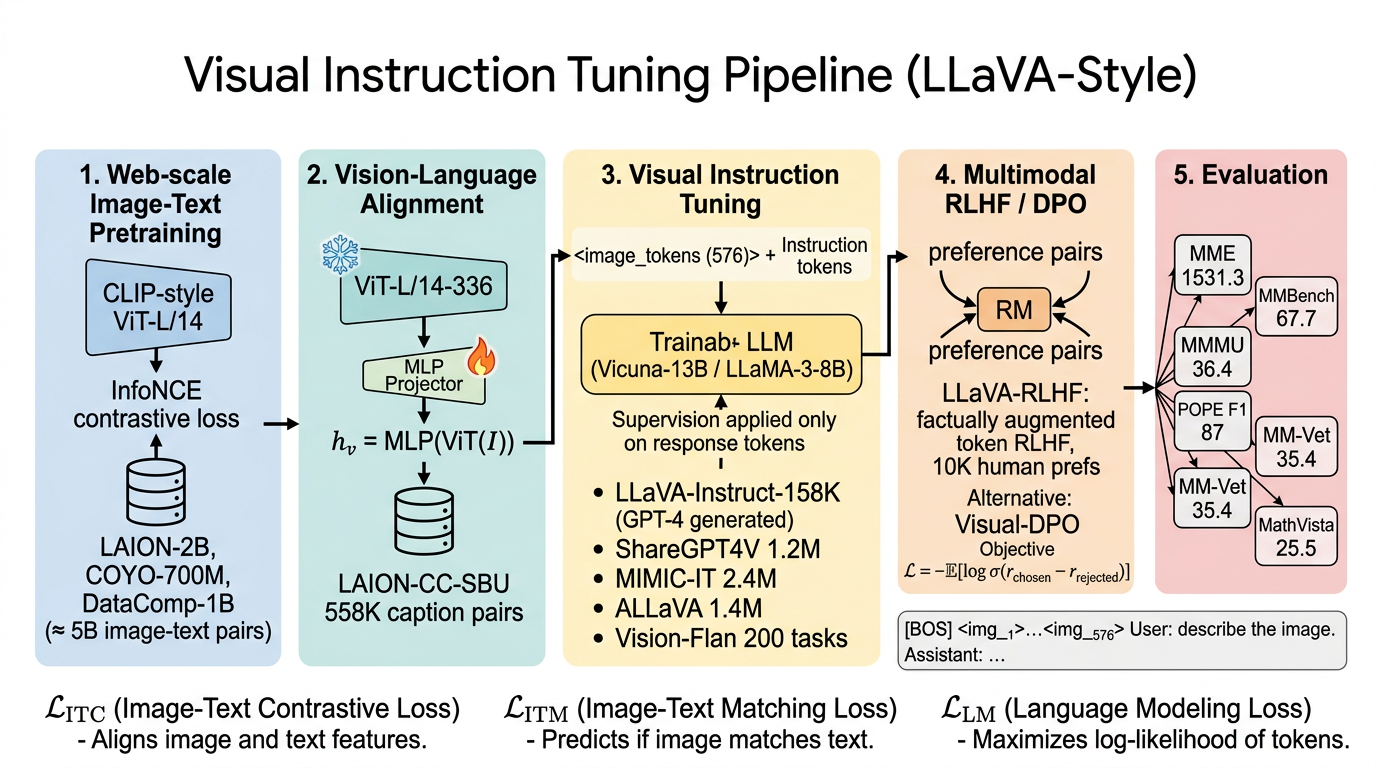
\includegraphics[width=\linewidth,keepaspectratio]{./figures/Multimodal-Large-Language-Models__fig3_training_pipeline.png}}
\caption{Visual Instruction Tuning Pipeline (LLaVA-style): five stages from web-scale image-text pretraining → vision-language alignment with a frozen ViT and trainable MLP projector → visual instruction tuning on 158K--10M GPT-4-generated triples → multim.}\label{fig:fig3-training-pipeline}\end{figure}

Whereas Section 3 catalogued the architectural choices, this section describes how those architectures are trained. This section reviews the four-stage training pipeline that has become the de facto MLLM recipe --- vision pretraining, connector alignment, visual instruction tuning, and preference optimisation --- together with parameter-efficient adaptation and the empirical scaling lessons that follow.

The dominant MLLM recipe is a four-stage pipeline that decouples what is seen (vision pretraining), how it is seen (connector alignment), how it is talked about (visual instruction tuning), and how it is corrected (preference learning). Concrete instantiations vary in scale but not in shape: LLaVA-1.5 reuses a separately pretrained CLIP-ViT-L/14, aligns a 2-layer MLP on 558K LAION-CC-SBU caption pairs, instruction-tunes on 665K mixed triples (158K LLaVA-Instruct + VQAv2/GQA/OK-VQA/TextVQA + RefCOCO + OCRVQA), and skips RLHF; LLaVA-RLHF adds a fourth stage with 10K factually augmented preferences and reduces MMHal hallucination by 60\%. InternVL-1.5/2.5 scales the alignment corpus to 1.3B pairs and the instruction stage to 5M samples; Qwen2-VL pretrains end-to-end on 1.4T tokens of interleaved image-text data with multimodal RoPE for 16,384 visual tokens. The community has converged on these stages between 2023 and 2026; we walk through each with the parameter counts, datasets, objectives, and ablation deltas that anchor reproducible comparison.

\subsection{Stage 1: Vision-Language Pretraining Objectives (ITC, ITM, ITG, MIM)}\label{stage-1-vision-language-pretraining-objectives-itc-itm-itg-mim}

The first stage usually predates MLLM training: the vision encoder is borrowed from a separately pretrained CLIP or SigLIP model. The dominant losses are:

\begin{itemize}

\item
  \textbf{Image-Text Contrastive (ITC)} --- symmetric InfoNCE over batches of paired (image, text), pushing matched pairs together and unmatched apart. This is the CLIP/ALIGN loss.
\item
  \textbf{Image-Text Matching (ITM)} --- a binary classifier that predicts whether an (image, text) pair matches, with hard-negative sampling.
\item
  \textbf{Image-grounded Text Generation (ITG)} --- autoregressive captioning of the image (used in CoCa, BLIP-2, BLIP-3).
\item
  \textbf{Masked Image Modelling (MIM)} --- masked-patch reconstruction (BEiT-3, DINOv2). DINOv2 \citep{oquab20232023} trained on 142M curated images shows strong dense-prediction features that some MLLMs (e.g., BRAVE) use alongside CLIP.
\end{itemize}

Combined objectives such as \(\mathcal{L} = \mathcal{L}_{\text{ITC}} + \mathcal{L}_{\text{ITM}} + \mathcal{L}_{\text{ITG}}\) in BLIP-2's stage 1 produce a Q-Former that already captures rich image semantics before any LLM is attached. Recent work suggests that \emph{captioner-supervised} contrastive learning (training on synthetic GPT-4V captions for LAION images) outperforms raw web alt-text by up to 10 points on dense-VQA benchmarks (Anasosalu Vasu et al., 2024). The \emph{vision-side scaling law} observed by InternVL \citep{chen20242024} is that doubling the vision encoder from 1B to 6B (InternViT-6B) yields +3.4 MMBench at fixed downstream training, while doubling input resolution from 224² to 448² yields +5.1 on TextVQA.

\subsection{Stage 2: Vision-Text Alignment via Projection or Q-Former Distillation}\label{stage-2-vision-text-alignment-via-projection-or-q-former-distillation}

In stage 2, the connector is trained to map vision features into the LLM's token space using \emph{only} image-caption pairs, not instruction data. \textbf{LLaVA}'s stage 2 uses 558K image-caption pairs filtered from LAION-CC-SBU; only the linear projector is trainable; the loss is the standard autoregressive next-token prediction on the caption. \textbf{LLaVA-1.5} retains the same recipe with an MLP projector. \textbf{BLIP-2 stage 2} trains the Q-Former → LLM linear adapter with frozen ViT and frozen LLM, on 129M image-text pairs (LAION-115M + COCO + CC + SBU + VG). \textbf{InstructBLIP} keeps stage 2 of BLIP-2 unchanged. \textbf{InternVL-1.5} scales stage 2 to billions of pairs from LAION-en, LAION-zh, CC12M, COYO, COCO, with high-quality filtering producing about 1.3B usable pairs.

Stage 2 has three failure modes worth naming. \emph{Modality-gap collapse}: when the projector is too small or too few pairs are seen, the LLM ignores image tokens and language priors dominate. \emph{Caption blandness}: web alt-text is often ``image of \ldots{}'' or ``stock photo'' placeholders, producing models that describe images formulaically; this motivated ShareGPT4V \citep{chen20242024} to recaption 1.2M images with GPT-4V at \(\sim\)\$50K cost. \emph{Catastrophic LLM forgetting}: when the LLM is unfrozen too early, text-only benchmarks degrade. The community standard is to \emph{freeze the LLM} in stage 2 and unfreeze it only in stage 3.

\subsection{Stage 3: Visual Instruction Tuning (LLaVA-Instruct-158K, ShareGPT4V, MIMIC-IT)}\label{stage-3-visual-instruction-tuning-llava-instruct-158k-sharegpt4v-mimic-it}

This stage gives MLLMs their dialogue abilities. \textbf{LLaVA-Instruct-158K} is constructed by feeding COCO image captions and bounding boxes to GPT-4 (text-only, no vision) and asking it to generate three types of dialogue: (i) 58K \emph{conversation} samples --- multi-turn QA grounded in the captions, (ii) 23K \emph{detailed description} samples, (iii) 77K \emph{complex reasoning} samples. The output is text-only; pairing each sample with the original COCO image yields the (image, instruction, response) triples used in supervised fine-tuning. The training loss is the standard cross-entropy on response tokens only:
\[\mathcal{L}_{\text{IT}} = -\sum_{t \in \text{response}} \log p_\theta(y_t \mid y_{<t}, h_v, \text{prompt}).\]
\textbf{LLaVA-1.5} scales this to 665K mixed instructions, pulling in academic VQA datasets (VQAv2, GQA, OK-VQA, TextVQA, A-OKVQA), grounding (RefCOCO/+/g), OCR (OCRVQA), and 158K LLaVA-Instruct. \textbf{MIMIC-IT} (Otter, 2023) adds 2.4M multi-image and video instructions. \textbf{ShareGPT4V} contributes 1.2M GPT-4V-recaptioned image-text pairs \emph{plus} 100K conversation samples. \textbf{ALLaVA-4V} and \textbf{Cambrian-7M} push the corpus to 7M+ samples spanning 50+ skills (chart, document, science, code).

Empirically, \emph{data quality and diversity} dominate raw count once a few hundred thousand samples have been seen. The Vision-Flan study \citep{xu2023multimodallearning} shows that scaling from 0.6M to 200-task human-labelled instructions yields +5.2 MMBench-EN, while merely adding more LAION captions saturates near 1M. The same study finds that a 1:1 ratio of academic-task data to GPT-4V-generated dialogue gives the best balance between benchmark scores and free-form chat fluency.

\subsection{Stage 4: Multimodal RLHF, DPO, and Factual Alignment}\label{stage-4-multimodal-rlhf-dpo-and-factual-alignment}

This subsection reviews preference optimisation techniques that calibrate MLLMs after instruction tuning. Representative preference-optimisation methods include: LLaVA-RLHF (Sun et al., 2024, Factually Augmented RLHF with 10K human preferences and +60\% MMHal-Bench reduction), RLHF-V (2024, fine-grained human corrections converging in 1.4K preference pairs), Visual-DPO (2024, DPO with diffusion-noise negatives), POVID (2024, preference data via image-side perturbation), RLAIF-V (2024, GPT-4V or Gemini as reward annotator producing 100K+ preference pairs), Silkie (2024, distillation of preferences from multiple MLLM judges), MM-RLHF (2025, large-scale multimodal preference dataset), CSR (Chain of Self-Reward, 2024), and STIC (2024, self-training with image comprehension as reward). PPO trades off stability for compute, while DPO closes the form and removes the reward model, and GRPO further removes the value model by group-relative advantage.

Even after instruction tuning, MLLMs hallucinate, refuse legitimate questions, and answer over-confidently on adversarial images. The fix mirrors the LLM playbook: collect human or model-annotated preferences and apply RLHF or DPO. \textbf{LLaVA-RLHF} \citep{sun20242024} introduces \emph{Factually Augmented RLHF}. The method augments the reward model with image captions and image-grounded rationales so it can detect hallucination, then collects 10K human preferences. The result is a +60\% reduction in object hallucination on MMHal-Bench and +18.0 absolute on POPE-adversarial F1. \textbf{RLHF-V} (2024) collects fine-grained human corrections on individual segments of model output and applies dense Direct Preference Optimisation, converging in only 1.4K preference pairs. \textbf{Visual-DPO} and \textbf{POVID} apply DPO with synthetic preference pairs constructed by perturbing the image (for example, adding diffusion noise to push the model into hallucinating) and using the original image as the preferred condition. \textbf{RLAIF-V} uses GPT-4V or Gemini as a reward annotator at scale, producing 100K+ preference pairs at near-zero human cost. Across these methods, post-training raises POPE F1 from about 85 to about 90 and reduces HallusionBench failure rates by 30--40\%.

\subsection{Parameter-Efficient Adaptation: LoRA, LLaMA-Adapter, Visual Prompt Tuning}\label{parameter-efficient-adaptation-lora-llama-adapter-visual-prompt-tuning}

A parallel line of work asks how to obtain MLLM behaviour at the lowest possible parameter cost. \textbf{LLaMA-Adapter} \citep{zhang2023videollamaaninstru} introduces \emph{zero-init attention} --- adapter prompts inserted into the upper LLM layers with a learned gating scalar initialised at zero so the LLM is unchanged at the start of training; with only 1.2M trainable params, LLaMA-Adapter matches Alpaca on text-only benchmarks. \textbf{LLaMA-Adapter V2} \citep{gao20232023} adds a vision branch by treating CLIP image features as a soft prompt, raising trainable parameters to 14M. \textbf{BLIVA} \citep{hu20242024} freezes BLIP-2 and adds visual prompt embeddings, recovering most of the OCR gap on TextVQA. \textbf{MiniGPT-4} trains only its single linear projector after stage 1; the entire stage-2 fine-tune uses 3,500 hand-curated pairs and converges in under one A100-day. \textbf{LLaVA Steering} (Bi et al., 2024) uses linear representation steering to achieve LLaVA-1.5 quality with 500× fewer trainable parameters, and is among the most aggressive PEFT recipes published.

LoRA-based MLLMs are now standard in academic settings. The trade-off observed by Laurençon et al.~(2024, IDEFICS-2 study) is that LoRA-only fine-tuning underperforms full fine-tuning by 2.4 points on MMBench at the 8B scale, but gives 70\% lower memory and is feasible on 4×A100 80GB. For frontier-quality results, full fine-tuning of the LLM remains necessary.

\subsection{Compute and cost ledger}\label{compute-and-cost-ledger}

\begin{table*}[t]
\centering
\caption{Compute and cost ledger: Model, Params (act.), Pretrain compute, Stage-3 data.}
\label{tab:compute-and-cost-ledger}
\begin{tabular}{>{\raggedright\arraybackslash}p{0.2358\linewidth}
  >{\raggedright\arraybackslash}p{0.1604\linewidth}
  >{\raggedright\arraybackslash}p{0.2358\linewidth}
  >{\raggedright\arraybackslash}p{0.1604\linewidth}
  >{\raggedright\arraybackslash}p{0.2075\linewidth}}
\toprule
\textbf{Model} & \textbf{Params (act.)} & \textbf{Pretrain compute} & \textbf{Stage-3 data} & \textbf{GPU-hours stage 3} \\
\midrule
LLaVA-1.5-13B & 13B & -- (uses Vicuna) & 665K & ≈ 26 h on 8×A100 \\
InstructBLIP (FlanT5-XXL) & 12B & -- (BLIP-2 reuses) & 1.2M & ≈ 100 h on 16×A100 \\
Qwen-VL-Chat & 9.6B & 1.4B image-text pairs & 350K & ≈ 1k h on 64×A100 \\
InternVL-1.5 & 26B & 1.3B pairs & 5M & ≈ 6k h on 256×H800 \\
Flamingo-80B & 80B & 1.8B noisy + M3W 43M & none (in-context) & 1.4M TPUv4-hours total \\
Chameleon-30B & 30B & 4.4T text + 1.4T VQ image & -- & ≈ 1.8M GPU-hours total \\
Janus-Pro-7B & 7B & 90M und + 72M gen & 1.2M & ≈ 5k H100-hours \\
\end{tabular}
\end{table*}

\subsection{Loss equations summary}\label{loss-equations-summary}

Stage 1: \(\mathcal{L} = \mathcal{L}_{\text{ITC}} + \mathcal{L}_{\text{ITM}} + \mathcal{L}_{\text{ITG}}\).
Stage 2: \(\mathcal{L} = -\sum_t \log p_\theta(y_t^{\text{cap}} \mid y_{<t}, h_v)\) (frozen LLM in BLIP-2 / Flamingo; trainable connector only).
Stage 3: \(\mathcal{L}_{\text{IT}} = -\sum_{t \in \text{response}} \log p_\theta(y_t \mid y_{<t}, h_v, \text{instr})\) (instruction masked from supervision).
Stage 4 RLHF: \(\max_\theta \mathbb{E}[r_\phi(x, y) - \beta \, \text{KL}(p_\theta \| p_{\text{ref}})]\) with PPO; or DPO closed-form: \(\mathcal{L}_{\text{DPO}} = -\mathbb{E}_{(x,y_w,y_l)}\left[\log \sigma\!\left(\beta \log \frac{p_\theta(y_w|x)}{p_{\text{ref}}(y_w|x)} - \beta \log \frac{p_\theta(y_l|x)}{p_{\text{ref}}(y_l|x)}\right)\right]\).

\subsection{Empirical scaling lessons}\label{empirical-scaling-lessons}

Three robust trends emerge from cross-paper comparison. \emph{First}, instruction-data quality saturates the model rapidly: going from 0 to 158K instructions yields +12 MMBench, but 158K to 1.2M only adds another +3, while curating the 158K with GPT-4V (ShareGPT4V) adds another +2 with no scale change. \emph{Second}, \emph{vision-tower scale} and \emph{LLM scale} contribute roughly additively in the 7--80B range; doubling either yields +3--6 MMBench. \emph{Third}, \emph{RLHF/DPO} has the highest score-per-FLOP at this point in the field --- 10K preference pairs add as much hallucination resistance as adding 5M instruction samples. These lessons motivate the data ecosystem and benchmark protocols described in Sections 6 and 7.

\section{Modality-Specific MLLMs Beyond Image-Text}\label{modality-specific-mllms-beyond-image-text}

Whereas Section 4 focused on the image--text training pipeline, this section turns to MLLMs built for video, audio, document, 3D, and robotic-action modalities. This section reviews each modality branch with its tokenisation strategy, encoder choice, alignment data, benchmark suite, and 2025 state of the art.

The image-text MLLM is only the largest and most studied node in a wider design space. Each additional modality --- video, audio, document, 3D, action --- introduces its own tokenisation problem, encoder choice, alignment data, and benchmark suite, and each branch trails image-text by 1--2 capability years. Video-LLaVA and VideoLLaMA-2 reach 70.7\% MSVD-QA and 54.6 Video-MME long at 7B; SALMONN attaches Whisper-large-v2 (1.5B) and BEATs (90M) to Vicuna-13B and emits 96 audio tokens per second; mPLUG-DocOwl reaches 62.2 ANLS on DocVQA via a layout-aware projector while frontier MLLMs now exceed 95 ANLS at 4K dynamic resolution; 3D-LLM and Point-LLM push MLLMs onto ScanQA (best result 27.3); RT-2 and OpenVLA close the loop to robot action through 1M episodes of Open X-Embodiment trajectories. The recurring lesson is that the modality with the worst supervision dominates failure modes --- audio MLLMs hallucinate music genres far more than image MLLMs hallucinate dog breeds because audio captions are sparser and noisier. The following subsections walk through each modality, naming the systems, encoders, token budgets, and benchmark numbers that anchor 2025-era comparison.

\subsection{Video MLLMs: Video-LLaMA, Video-LLaVA, VideoLLaMA-2, mPLUG-Owl3}\label{video-mllms-video-llama-video-llava-videollama-2-mplug-owl3}

This subsection reviews video MLLMs and the long-video gap. Representative video MLLMs include: Video-LLaMA (June 2023, video-Q-Former plus audio-Q-Former on EVA-CLIP and ImageBind), Video-ChatGPT (June 2023, spatiotemporal pooling on Vicuna), VideoChat (May 2023, video-text foundation with TimeChat tokens), Video-LLaVA (November 2023, LanguageBind unified encoder reaching 70.7\% MSVD-QA), VideoLLaMA-2 (June 2024, Spatial-Temporal Convolutional connector reaching 54.6 Video-MME long), mPLUG-Owl3 (August 2024, hyper-attention scaling to 8 hours of video), InternVideo2 (2024, 1B-parameter video foundation trained on 412M videos), LLaVA-Video (2024, synthetic-data scaling to 178K video-text pairs), LongVA (2024, ring-attention for long video), VideoChat-T (2024, chain-of-shot reasoning), Kangaroo (2024, long-context video MLLM), and ShareGPT4Video (2024, GPT-4V-recaptioned video corpus).

Video adds a temporal axis that explodes the visual-token budget. The pragmatic baseline samples \(T\) frames (typically 4--32), encodes each with the image MLLM's vision tower, and pools or concatenates frame features before the connector. \textbf{Video-LLaMA} \citep{zhang2023videollamaaninstru} couples a video-Q-Former with an audio-Q-Former on top of EVA-CLIP and ImageBind, instruction-tuning on 11K WebVid-derived video-text pairs and 5K audio-text pairs. \textbf{Video-LLaVA} \citep{lin20242024} aligns image and video features \emph{before} projection by training the LanguageBind unified encoder on combined image and video corpora, eliminating the need for separate stage-2 alignment for each modality; on MSVD-QA it reaches 70.7\% (zero-shot) and outperforms frame-stacking baselines by 3--5 absolute. \textbf{VideoLLaMA-2} \citep{cheng20242024} introduces a Spatial-Temporal Convolutional connector and adds audio understanding from a separate Whisper-Audio branch, reporting 54.6 on Video-MME (long subset) at the 7B scale. \textbf{mPLUG-Owl3} \citep{ye20242024} extends single-image MLLMs to up to 8 hours of video by interleaving 128 sparse frames with adaptive temporal compression. \textbf{InternVideo2} \citep{wang20242024} trains a 1B-parameter video foundation model on 412M videos and serves as the vision tower for several video MLLMs. \textbf{LLaVA-Video} \citep{zhang20242024} uses synthetic-data scaling to 178K video-text pairs and demonstrates that careful synthetic data plus a frozen image MLLM matches more compute-intensive video-pretrained baselines.

Long-video benchmarks (Video-MME, EgoSchema, MLVU, LongVideoBench) reveal a sharp gap: models that excel on 1-minute clips fail on 1-hour content because the visual-token budget exceeds 16K tokens and key information is lost in pooling. \textbf{Gemini 1.5 Pro} uses its 1M-token context to ingest entire films (\textasciitilde2h at 1 fps), reaching 67.4\% on Video-MME long, while open-source models cluster in the 45--55\% range. Token compression methods (FastV, LLaVA-PruMerge, T*) and chain-of-shot prompting (CoS) \citep{hu20242024} attempt to close this gap on commodity hardware.

\subsection{Audio and Speech MLLMs: SALMONN, Qwen-Audio, SpeechGPT, AudioPaLM}\label{audio-and-speech-mllms-salmonn-qwen-audio-speechgpt-audiopalm}

This subsection reviews audio and speech MLLMs. Representative audio MLLMs include: SALMONN (2024, Whisper-large-v2 plus BEATs feeding a window-level Q-Former at 96 audio tokens per second), Qwen-Audio (2023, 30 audio tasks unified by task tags), Qwen2-Audio (2024, natural-language prompted audio LLM), SpeechGPT (2023, HuBERT discrete units in a unified spoken language Transformer), AudioPaLM (2023, unified text and audio token vocabulary), AudioGPT (2023, multi-tool ASR plus TTS plus audio-LLM pipeline), Pengi (2023, audio captioning and QA via prompt-driven prefix), LTU (2023, listen-think-understand audio reasoning), DeSTA2.5-Audio (2025, large-scale audio reasoning), WavLLM (2024, dual-encoder speech LLM), GAMA (2024, large audio-language model with multi-task instruction tuning), and GPT-4o (May 2024, first commercial unified speech-text MLLM with sub-300 ms voice latency).

Audio MLLMs face the same structural problem as video MLLMs: long sequences of high-dimensional features. \textbf{SALMONN} \citep{tang20242024} uses Whisper-large-v2 (1.5B) for speech and BEATs (90M) for general audio, combining both feature streams through a window-level Q-Former that emits 96 audio tokens per second of input, then attaches them as a soft prompt to Vicuna-13B. SALMONN supports speech recognition, speech translation, audio captioning, music understanding, emotion recognition, and zero-shot prompted audio tasks; it is the most general academic audio LLM at the time of writing. \textbf{Qwen-Audio} \citep{chu20232023} trains on 30 audio tasks unified into a single autoregressive sequence with task tags; \textbf{Qwen2-Audio} simplifies inference by using natural language prompts. \textbf{SpeechGPT} \citep{zhang2023videollamaaninstru} tokenises speech into HuBERT-derived discrete units and trains a unified spoken language Transformer with cross-modal instruction tuning, supporting multimodal speech chat. \textbf{AudioPaLM} uses a unified vocabulary for text and audio tokens. \textbf{AudioGPT}, \textbf{Pengi}, \textbf{LTU}, \textbf{DeSTA2.5-Audio} \citep{lu20242024}, and \textbf{WavLLM} are additional academic systems. \textbf{GPT-4o} (May 2024) is the first commercial deployment of a unified speech-text MLLM with sub-300ms latency for voice conversation.

Benchmarks include \textbf{AIR-Bench} \citep{yang20242024} --- 20 audio tasks across foundation and chat splits --- \textbf{MuChoMusic} for music understanding, and the \textbf{Whisper} WER suites for ASR. Open-source audio MLLMs have largely closed the ASR gap to Whisper-large but trail proprietary frontier on multi-step audio reasoning (e.g., ``what year is this song from and why?'').

\subsection{Document, Chart, and Table MLLMs: mPLUG-DocOwl, Kosmos-2.5, MatCha, ChartQA}\label{document-chart-and-table-mllms-mplug-docowl-kosmos-2.5-matcha-chartqa}

This subsection reviews document, chart, and table MLLMs. Representative document MLLMs include: mPLUG-DocOwl (2023, layout-aware projector reaching DocVQA 62.2 ANLS), mPLUG-DocOwl 1.5 (2024, chart and table understanding), DocPedia (2023, frequency-domain DCT features for 2,560² images), DocLLM (2023, layout-aware bounding-box conditioning for forms and receipts), DocKylin (2025, visual slimming for document MLLMs), Kosmos-2.5 (2023, ``multimodal literate model'' with unified Markdown output on 357M document pairs), MatCha (2023, math reasoning plus chart de-rendering pretraining beating ChartQA by 6 points), UniChart (2023, unified chart-grounded foundation), ChartReader (2023, structured chart parsing), ChartLlama (2024, GPT-4V-distilled chart instruction set), TableLLaVA (2024, table-image instruction tuning), TextMonkey (2024, document-image MLLM with shifted-window attention), and HRVDA (2024, high-resolution visual document assistant).

Documents, charts, and tables are arguably the most economically valuable MLLM application after general visual chat: enterprises run terabytes of PDFs through them. The challenge is dense, small text and structured layout. \textbf{mPLUG-DocOwl} \citep{ye20232023} extends mPLUG-Owl with document images and a layout-aware projector; on DocVQA it reaches 62.2 ANLS (zero-shot). \textbf{DocPedia} (Feng et al., 2023) operates in the \emph{frequency domain} using DCT features to handle 2,560×2,560 images without prohibitive token counts. \textbf{DocLLM} \citep{wang20232023} is layout-aware and conditions on bounding-box tokens rather than image features, simplifying the architecture for forms, invoices, and receipts. \textbf{DocKylin} \citep{zhang20242024} introduces visual slimming for document MLLMs. \textbf{Kosmos-2.5} \citep{lv20232023} is a ``multimodal literate model'' trained for full document image transcription with a unified Markdown output format, on 357M document image-text pairs. \textbf{mPLUG-DocOwl 1.5} (2024) adds chart-table understanding. \textbf{MatCha} \citep{liu2023visualinstructiont} injects math reasoning and chart de-rendering as auxiliary tasks during pretraining and beats competitive baselines on ChartQA by 6 points absolute. \textbf{UniChart} (Masry et al., 2023) and \textbf{ChartReader} \citep{cheng20242024} further specialise on chart understanding.

The benchmark suite for this branch includes \textbf{DocVQA} (50K Q over 12K document images, ANLS metric), \textbf{ChartQA} (32K Q), \textbf{InfographicVQA}, \textbf{AI2D}, \textbf{TabFact}, and \textbf{ScienceQA}. Frontier MLLMs now achieve \textgreater90 ChartQA (GPT-4o 86.7, InternVL-2.5 88.6) and \textgreater85 DocVQA (Qwen2-VL 95.4 with high-resolution dynamic input).

\subsection{3D, Point Cloud, and Scene MLLMs: Point-LLM, 3D-LLM, LL3DA}\label{d-point-cloud-and-scene-mllms-point-llm-3d-llm-ll3da}

This subsection reviews 3D and scene MLLMs. Representative 3D MLLMs include: 3D-LLM (2023, scene representations projected via 3D feature extractor and Q-Former), Point-LLM (2023, sparse-conv point-cloud encoder), LL3DA (2023, interactor for click-based region specification), PointLLM (2023, 6M point-cloud-text instruction tuning), Chat-3D (2023, 3D scene captioning and QA), LEO (2024, embodied 3D agent with scene graph reasoning), SceneVerse (2024, 2.5M scene-text pairs), 3D-VisTA (2023, pretrained vision-text alignment for 3D), and Grounded-3D-LLM (2024, language-grounded 3D detection and segmentation).

3D MLLMs ingest point clouds, voxel grids, or multi-view images. \textbf{3D-LLM} projects scene representations into a frozen LLM via 3D feature extractor + Q-Former; \textbf{Point-LLM} treats raw point clouds with a sparse-conv encoder. \textbf{LL3DA} introduces an interactor that lets users specify regions through clicks. Benchmarks remain comparatively small (ScanQA, SQA3D, ScanRefer, 3D-MV-Bench). 3D MLLMs are essential for embodied applications (Section 8.3) but lag image MLLMs by roughly two years in capability.

\subsection{Any-to-Any and Unified U+G Models: NExT-GPT, ImageBind-LLM, Janus-Pro}\label{any-to-any-and-unified-ug-models-next-gpt-imagebind-llm-janus-pro}

This subsection reviews any-to-any and unified understanding-and-generation MLLMs. Representative any-to-any systems include: NExT-GPT (2024, ImageBind plus Vicuna plus three diffusion decoders for image, audio, and video output), ImageBind-LLM (2023, instruction-tuning LLaMA on the bound 6-modality ImageBind embedding space), AnyGPT (2024, unified discrete tokens for image, audio, music, and text), CoDi (2023, composable diffusion across modalities), CoDi-2 (2024, in-context interleaved any-to-any generation), Chameleon (2024, mixed-modal early-fusion at 7B and 30B), Show-o (2024, autoregressive text plus discrete diffusion images), Janus (2024, decoupled understanding and generation encoders), Janus-Pro-7B (2025, MMMU 41.0 and GenEval 0.80), Liquid (2024, single autoregressive Transformer at 7B and 32B), and Emu3 (2024, next-token prediction across image, text, and video).

The most ambitious axis is ``any to any'' --- accepting and producing arbitrary modalities. \textbf{NExT-GPT} \citep{wu20242024} connects ImageBind (which binds 6 modalities --- image, text, audio, video, depth, thermal, IMU --- into one space) to Vicuna and adds three diffusion decoders (Stable Diffusion for images, AudioLDM for audio, Zeroscope for video), tied with a learned linear projection on each side. \textbf{ImageBind-LLM} \citep{han20232023} instruction-tunes LLaMA on the bound embedding space for 5 modalities. \textbf{AnyGPT} uses unified discrete tokens for image, audio, music, and text, training a single autoregressive Transformer. \textbf{CoDi} and \textbf{CoDi-2} (2023--2024) are diffusion-based any-to-any frameworks. As discussed in Section 3.4, recent unified U+G models (Chameleon, Show-o, Janus, Janus-Pro, Liquid) take a different stance --- VQ-tokenise everything and train one Transformer --- and have produced the strongest combined understanding-and-generation numbers to date. \textbf{Janus-Pro-7B} reports MMMU 41.0, MMBench 79.2, GenEval 0.80, FID-COCO 8.4, the first open model to be simultaneously competitive on understanding and on text-to-image generation.

\begin{table*}[t]
\centering
\caption{Any-to-Any and Unified U+G Models: NExT-GPT, ImageBind-LLM, Janus-Pro: Modality, Representative MLLM, Encoder, Tokens / second or per input.}
\label{tab:any-to-any-and-unified-u-g-models-next-gpt-imagebind-llm-jan}
\begin{tabular}{>{\raggedright\arraybackslash}p{0.0795\linewidth}
  >{\raggedright\arraybackslash}p{0.2102\linewidth}
  >{\raggedright\arraybackslash}p{0.1989\linewidth}
  >{\raggedright\arraybackslash}p{0.1818\linewidth}
  >{\raggedright\arraybackslash}p{0.0909\linewidth}
  >{\raggedright\arraybackslash}p{0.2386\linewidth}}
\toprule
\textbf{Modality} & \textbf{Representative MLLM} & \textbf{Encoder} & \textbf{Tokens / second or per input} & \textbf{Benchmark} & \textbf{State of the art (2025)} \\
\midrule
Image & LLaVA-1.5, GPT-4V & CLIP-ViT-L/14, SigLIP, InternViT-6B & 576--4096 & MMBench-EN & 84.6 (DeepSeek-VL2), 86.7 (Gemini 1.5 Pro) \\
Video & Video-LLaVA, VideoLLaMA-2, mPLUG-Owl3 & VideoMAE, EVA-CLIP frame & 512--16K per minute & Video-MME long & 67.4 (Gemini 1.5 Pro), 56.5 (Qwen2-VL-72B) \\
Speech & SALMONN, Qwen-Audio, GPT-4o & Whisper, BEATs & 96/s (SALMONN) & LibriSpeech WER & 1.7\% (Whisper-large), GPT-4o ≈ 1.8\% \\
Audio events & SALMONN, AudioGPT & BEATs, AudioMAE & 96/s & AudioCaps SPIDEr & 0.49 (SALMONN) \\
Music & Qwen-Audio, MusicLM & MERT, AudioMAE & 96/s & MuChoMusic & 0.71 acc \\
3D & 3D-LLM, Point-LLM & PointBERT, BERT-3D & 512 tokens & ScanQA & 27.3 (3D-LLM) \\
Action / Robot & RT-2, OpenVLA & ViT + tokeniser & 128 & RT-2 sim & 62\% generalisation \\
Any-to-any & NExT-GPT, AnyGPT & ImageBind, VQ codebooks & varies & MM-Generation & 0.80 GenEval (Janus-Pro) \\
\end{tabular}
\end{table*}

\subsection{Cross-modality alignment data}\label{cross-modality-alignment-data}

Large multi-modal alignment data is the bottleneck for non-image branches. \textbf{WebVid-2.5M} and \textbf{InternVid} (Wang et al., 2023, 234M video clips) anchor video; \textbf{AudioSet-2M}, \textbf{WavCaps}, \textbf{Clotho}, and \textbf{MACS} anchor audio; \textbf{Objaverse-XL} (10M 3D objects) and \textbf{ScanScribe} anchor 3D; \textbf{RT-X} (Embodiment Collaboration, 2023, 1M episodes from 22 robots and 60 datasets) anchors embodied action. Multi-modal MLLM data construction is itself a research area --- Qin et al.~(2025) survey the \emph{co-development} relationship between data and MLLMs, noting that synthetic data filtration with a strong MLLM as judge has become standard practice.

\subsection{Why modality matters for system design}\label{why-modality-matters-for-system-design}

Three lessons recur. \emph{First}, every additional modality requires re-tokenisation and re-alignment; there is no free lunch from a ``unified'' encoder unless the binding loss is carefully chosen. \emph{Second}, the \emph{modality with the worst supervision} tends to dominate failure modes --- audio MLLMs hallucinate music genres far more than image MLLMs hallucinate dog breeds because audio captions are sparser. \emph{Third}, \emph{unified U+G} models have shown that the right discretisation lets one Transformer span several modalities, but at a 2--6 point understanding cost relative to specialised MLLMs. We anticipate this gap to close by 2026--2027 as VQ codebooks mature, but it will not close trivially.

\section{Datasets and Data Construction Pipelines}\label{datasets-and-data-construction-pipelines}

Building on the modality branches in Section 5, this section catalogues the corpora that train them. This section reviews four data scales --- web-scale alignment pairs, interleaved image--text documents, curated instruction triples, and domain-specific corpora --- together with the cross-corpus lessons that drive 2025--2026 training decisions.

If MLLMs have a single secret ingredient, it is data --- both the multi-billion-pair alignment corpora that produce strong vision encoders and the carefully curated instruction sets that produce dialogue fluency. The data ecosystem now spans four scales: web-scale alignment (LAION-5B at 5.85B pairs, COYO-700M at 747M, DataComp-1B at 1.4B filtered pairs); interleaved image-text documents (OBELICS at 141M docs and 353M images; OmniCorpus at 8.6B images and 1.7T tokens); curated instruction triples (LLaVA-Instruct-158K, ShareGPT4V's 1.2M GPT-4V recaptions, Cambrian-7M, ALLaVA-4V at 1.4M, Vision-Flan's 200-task human-labelled set); and domain corpora (MIMIC-CXR's 377K chest X-ray pairs, RT-X's 1M robot episodes, NuScenes-QA's 460K driving questions, ScienceQA's 21,208 K-12 multimodal MCQs). Cross-corpus ablations show that data quality saturates faster than data quantity once instruction tuning enters the picture: ShareGPT4V's recaptioning yields +1.4 MMBench-EN at fixed compute over LAION-CC-SBU, while the Vision-Flan study reports +5.2 MMBench-EN from scaling task diversity from 0.6M to 200-task human instructions. This section catalogues the major corpora, the construction pipelines, and the cross-corpus lessons that drive 2025--2026 MLLM training decisions.

\subsection{Web-Scale Image-Text Corpora: LAION-5B, COYO-700M, DataComp-1B}\label{web-scale-image-text-corpora-laion-5b-coyo-700m-datacomp-1b}

This subsection reviews web-scale image--text corpora. Representative web-scale corpora include: Conceptual Captions 3M (CC3M, 2018, 3M alt-text pairs), Conceptual Captions 12M (CC12M, 2021, 12M scraped pairs), WIT (2021, 37.6M Wikipedia image--text aligned across 108 languages), LAION-400M (2021, first publicly downloadable CLIP-filtered set at 400M pairs), LAION-2B-en (2022, English subset of 2.32B pairs), LAION-5B (2022, 5.85B pairs across languages), COYO-700M (Kakao Brain, 2022, 747M English pairs), DataComp-1B (Gadre et al., 2023, 1.4B pairs from competition-driven filtering), LAION-COCO 600M (2022, BLIP-recaptioned LAION subset), DFN (2023, data-filtering networks producing high-quality pretraining data), MetaCLIP (2024, transparent reproduction of the CLIP curation recipe), DALLE-3 captions (2024, dense captions from a strong captioner), and Re-LAION-2B (2024, safety-filtered re-release).

The vision-language community moved from millions to billions of pairs in two steps. \textbf{Conceptual Captions 3M (CC3M)} (Sharma et al., 2018) and \textbf{CC12M} scraped Web alt-text. \textbf{WIT} (Wikipedia Image-Text, Srinivasan et al., 2021) provides 37.6M images aligned with multilingual captions across 108 languages. \textbf{LAION-400M} (Schuhmann et al., 2021) and \textbf{LAION-2B-en / LAION-5B} (2022) opened the floodgates by releasing publicly downloadable image-text pairs filtered by CLIP similarity ≥ 0.28. \textbf{COYO-700M} (Kakao Brain, 2022) is a comparable English-language dataset of 747M pairs. \textbf{DataComp-1B} (Gadre et al., 2023) is the first dataset built around an \emph{open competition}: a fixed compute budget on a fixed training pipeline, allowing principled comparison of filtering strategies. \textbf{LAION-COCO 600M} is a synthetic recaptioning of LAION using BLIP, providing higher-quality but less diverse captions. \textbf{DataComp} experiments showed that aggressive filtering of noisy data can match the accuracy of training on 4× more raw pairs, an inversion of the ``more data is always better'' intuition.

These corpora are noisy: typical captions are alt-text fragments, marketing copy, or entity names. Their value lies in \emph{scale} --- the contrastive loss needs hundreds of millions of pairs to push image and text into a shared cone in the embedding space, after which downstream alignment can be done with much smaller, cleaner sets.

\subsection{Interleaved Image-Text Documents: OBELICS, MMC4, WIT}\label{interleaved-image-text-documents-obelics-mmc4-wit}

This subsection reviews interleaved image--text corpora that enable few-shot in-context multimodal learning. Representative interleaved corpora include: M3W (2022, 43M Flamingo pretraining webpages with 185M images, proprietary to DeepMind), OBELICS (HuggingFace, 2023, 141M English documents with 353M images and 115B text tokens), MMC4 (Multimodal C4, 2023, 41.6M documents with 571M images), OmniCorpus (2024, 8.6B images and 1.7T text tokens), MINT-1T (2024, 1T-token public interleaved corpus with PDF and HTML), CapsFusion (2024, 120M caption-fused interleaved documents), VisualCorpus (2024, curated interleaved set for academic benchmarking), and InterleavedQA (2024, multi-image QA corpus).

Modern MLLMs benefit from \emph{interleaved} image-text data --- webpages, papers, and tutorials where multiple images are placed in sentence context --- because this format is the closest analogue to the multi-image dialogues users actually have. \textbf{OBELICS} (HuggingFace, 2023) is 141M English-language web documents containing 353M images with their surrounding text, totalling 115B text tokens; this is the corpus that powers IDEFICS-1/2/3. \textbf{MMC4} (Multimodal C4, Zhu et al., 2023) is 41.6M documents with 571M images derived from Common Crawl C4. \textbf{OmniCorpus} (2024) extends this to 8.6B images and 1.7T text tokens. \textbf{InterleavedQA} and \textbf{VisualCorpus} are smaller curated sets used in academic benchmarking. Flamingo's M3W (43M webpages with 185M images) was the original interleaved corpus and remains proprietary to DeepMind. Models trained with interleaved data exhibit dramatically stronger few-shot in-context multimodal learning than caption-only models --- Flamingo's signature ability to learn a new visual classification task from 4 examples in-context comes directly from M3W exposure.

\subsection{Synthetic Caption and Instruction Data: ShareGPT4V, ALLaVA, Cambrian}\label{synthetic-caption-and-instruction-data-sharegpt4v-allava-cambrian}

This subsection reviews synthetic instruction and caption corpora. Representative instruction corpora include: LLaVA-Instruct-158K (2023, GPT-4 dialogues over COCO captions), ShareGPT4V (2024, 1.2M GPT-4V recaptions averaging 942 characters), MIMIC-IT (2023, 2.4M multi-image and video instructions), ALLaVA-4V (2024, 1.4M GPT-4V triples covering 50+ skills), Cambrian-7M (2024, 7M instructions from 26 sources), LLaVA-OneVision (2024, 10M+ multi-domain instructions including multi-image and video), Vision-Flan (2024, 200-task human-labelled instructions, 1.6M samples), Math-PUMA (2025, progressive math instruction data with diagram alignment), DataComp-LM (2024, instruction-data filtering competition), LRV-Instruction (2024, robust instruction tuning), and Sphinx (2024, multi-task multi-vision instruction set).

Once strong MLLMs existed, the community used them to generate the data for the next generation. \textbf{LLaVA-Instruct-158K} \citep{liu2023visualinstructiont} was generated by GPT-4 (text-only) given COCO captions and bounding boxes as a textual proxy for the image. \textbf{ShareGPT4V} \citep{chen20242024} used GPT-4V (with vision) to recaption 1.2M images with detailed captions averaging 942 characters; pretraining on ShareGPT4V instead of LAION-CC-SBU yields +1.4 MMBench-EN at fixed compute and +3.0 on TextVQA. \textbf{MIMIC-IT} (Otter, 2023) is 2.4M instructions across multi-image and video, much of it generated by GPT-4. \textbf{ALLaVA-4V} (2024) is 1.4M GPT-4V triples covering 50+ skills. \textbf{Cambrian-7M} (Tong et al., 2024) is the largest single-source instruction set at 7M samples constructed from 26 diverse academic and synthetic sources. \textbf{LLaVA-OneVision} (2024) consolidated 10M+ multi-domain instructions including images, multi-image bursts, and video. \textbf{Vision-Flan} \citep{xu2023multimodallearning} takes a different stance --- collecting \emph{human-labelled} task-diverse instructions from 200 tasks --- and demonstrates that scaling task diversity matters more than scaling per-task data. \textbf{Math-PUMA} (Zhuang et al., 2025) constructs progressive math instruction data with diagram alignment.

\begin{table*}[t]
\centering
\caption{Synthetic Caption and Instruction Data: ShareGPT4V, ALLaVA, Cambrian: Corpus, Type, Size, Year.}
\label{tab:synthetic-caption-and-instruction-data-sharegpt4v-allava-cam}
\begin{tabular}{>{\raggedright\arraybackslash}p{0.1939\linewidth}
  >{\raggedright\arraybackslash}p{0.2347\linewidth}
  >{\raggedright\arraybackslash}p{0.2143\linewidth}
  >{\raggedright\arraybackslash}p{0.0816\linewidth}
  >{\raggedright\arraybackslash}p{0.2755\linewidth}}
\toprule
\textbf{Corpus} & \textbf{Type} & \textbf{Size} & \textbf{Year} & \textbf{Use} \\
\midrule
LAION-5B & image-text pairs & 5.85B & 2022 & CLIP-style stage 1 \\
COYO-700M & image-text pairs & 747M & 2022 & stage 1 alternative \\
LAION-COCO & synthetic captions & 600M & 2022 & recaption baseline \\
DataComp-1B & filtered pairs & 1.4B & 2023 & optimal filtering benchmark \\
WIT & multilingual pairs & 37.6M & 2021 & multilingual MLLMs \\
OBELICS & interleaved web docs & 141M docs / 353M imgs & 2023 & IDEFICS-1/2/3 pretraining \\
MMC4 & interleaved web docs & 41.6M docs & 2023 & open Flamingo replication \\
OmniCorpus & interleaved & 8.6B images & 2024 & InternVL/Cambrian \\
LLaVA-Instruct-158K & dialogue triples & 158K & 2023 & LLaVA stage 3 \\
ShareGPT4V & GPT-4V captions+chat & 1.2M cap + 100K chat & 2024 & LLaVA-1.5+ stage 2/3 \\
MIMIC-IT & multi-image instruction & 2.4M & 2023 & Otter, video MLLMs \\
Cambrian-7M & instruction & 7M & 2024 & Cambrian-1 stage 3 \\
ALLaVA-4V & instruction & 1.4M & 2024 & open instruction tuning \\
Vision-Flan & human task instructions & 200 tasks, 1.6M & 2024 & task-diverse fine-tuning \\
InternVid & video-text & 234M clips & 2023 & video MLLMs \\
WebVid-10M & video-text & 10.7M clips & 2021 & video alignment \\
HD-VILA-100M & video-text & 100M clips & 2022 & video pretraining \\
WavCaps & audio caption & 403K & 2023 & SALMONN, Qwen-Audio \\
AudioSet-2M & audio events & 2M & 2017 & audio pretraining \\
RT-X & robot trajectories & 1M episodes & 2023 & VLA pretraining \\
MIMIC-CXR & medical & 377K image-report & 2019 & medical MLLMs \\
\end{tabular}
\end{table*}

\subsection{Domain-Specific Corpora: MIMIC-CXR, RT-X, NuScenes-QA, GMAI}\label{domain-specific-corpora-mimic-cxr-rt-x-nuscenes-qa-gmai}

This subsection reviews domain-specific corpora. Representative domain corpora include: MIMIC-CXR (2019, 377,110 chest X-ray image--report pairs), PMC-15M (2023, 15M biomedical figure--caption pairs from PubMed Central), GMAI-MMBench (2024, 38 medical datasets across 18 modalities and 18 anatomical regions, 26,675 samples), PathBench (2024, pathology MLLM benchmark), ReXVQA (2024, 694K chest-X-ray QA over 160K studies), NuScenes-QA (2024, 460K driving questions over 1000 scenes), AniDriveQA (2025, animal-presence driving QA), LingoQA (2024, planning-oriented driving QA), DriveLM-nuScenes (2024, perception--prediction--planning chain QA), RT-X / Open X-Embodiment (2023, 1M episodes across 22 robots and 60 datasets), DROID (2024, 76K robot trajectories), BridgeData V2 (2023, 60K manipulation trajectories), ScienceQA (2022, 21,208 K-12 multimodal MCQs with rationales), AI2D (2017, 5,000 science diagrams), Design2Code (2024, paired UI screenshots and HTML), and WebSight-1M (2024, 1M web designs).

Domain MLLMs require domain-aligned data. Medical: \textbf{MIMIC-CXR} (Johnson et al., 2019) provides 377,110 chest X-ray images paired with radiology reports --- the foundation for LLaVA-Med, Med-Flamingo, MedGemini, CheXmix, and ReXVQA. \textbf{PMC-15M} is a 15M biomedical figure-caption corpus from PubMed Central. \textbf{GMAI-MMBench} \citep{chen20242024} compiles 38 medical datasets across 18 modalities and 18 anatomical regions, totalling 26,675 samples. \textbf{PathBench} addresses pathology. Driving: \textbf{NuScenes-QA} \citep{qian20242024} builds on the nuScenes 1000-scene benchmark; \textbf{AniDriveQA} \citep{wang20242024} adds animal-presence scenarios; \textbf{LingoQA} and \textbf{DriveLM-nuScenes} add planning-oriented QA. Robotics: \textbf{RT-X} (Open X-Embodiment, 2023) is the largest cross-embodiment robotic dataset, 1M episodes spanning 22 robots and 60 datasets, with action labels in a unified end-effector space; \textbf{DROID} and \textbf{BridgeData V2} complement it. Education: \textbf{ScienceQA} (Lu et al., 2022) is 21,208 multimodal MC questions with rationales; \textbf{AI2D} is 5,000 science diagrams. Code/UI: \textbf{Design2Code} \citep{si20242024} provides paired UI screenshots and HTML; \textbf{WebSight-1M} generates 1M web designs. Each domain has a familiar pattern --- start from existing labelled data, add LLM-or-MLLM-generated explanations to produce instruction triples, and tune.

\subsection{Data construction lessons}\label{data-construction-lessons}

Six lessons recur across corpus papers. \emph{First}, \textbf{CLIP filtering} alone is insufficient at the instruction-tuning stage; semantic deduplication and aesthetic filtering matter (DataComp-1B). \emph{Second}, \textbf{synthetic captioning} with a strong MLLM (GPT-4V, Gemini, or Cambrian-1 itself) consistently improves downstream performance over alt-text. \emph{Third}, \textbf{interleaved data} is essential for in-context learning and multi-image tasks but costly to filter (OBELICS team report dropping 60\% during cleaning). \emph{Fourth}, \textbf{task diversity} dominates raw count once a few hundred thousand samples are seen (Vision-Flan). \emph{Fifth}, \textbf{synthetic preference data} (Visual-DPO, RLAIF-V) substitutes for costly human preferences in RLHF. \emph{Sixth}, \textbf{decontamination} of evaluation benchmarks from training data is now a documented problem --- Chen et al.~(2024) report that several models regress under MMMU-Pro's harder presentation when contamination is removed. Qin et al.~(2025) frame this as the \emph{co-development} of data and MLLMs and call for joint data-model evaluation, a position increasingly accepted in the community. Together, these lessons set up the benchmark landscape we examine next.

\section{Benchmarks and Evaluation Protocols}\label{benchmarks-and-evaluation-protocols}

\begin{figure}[t]
\centering
\pandocbounded{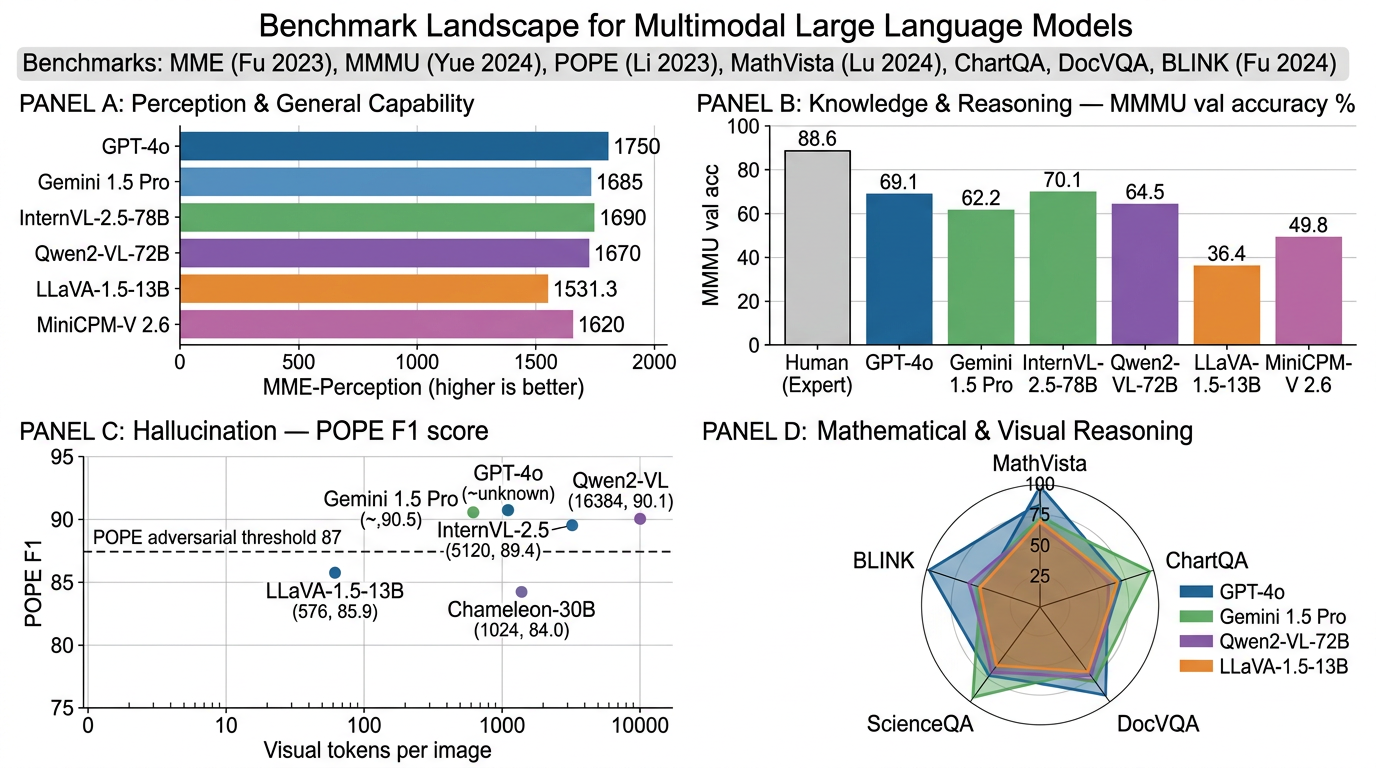
\includegraphics[width=\linewidth,keepaspectratio]{./figures/Multimodal-Large-Language-Models__fig4_benchmark_landscape.png}}
\caption{Benchmark landscape for Multimodal Large Language Models --- perception (MME, MMBench), knowledge \& reasoning (MMMU, MathVista), hallucination (POPE), and visual reasoning radar across GPT-4o, Gemini 1.5 Pro, InternVL-2.5, Qwen2-VL, LLaVA-1.5, an.}\label{fig:fig4-benchmark-landscape}\end{figure}

Whereas Section 6 catalogued training corpora, this section catalogues evaluation suites. This section reviews five benchmark clusters --- perception, knowledge and reasoning, hallucination, open-ended judging, and modality-or-domain-specific suites --- and ends with a frontier scoreboard and a discussion of contamination, visual reliance, and judge leakage.

The MLLM benchmark space has grown more rapidly than any other axis of the field, with dozens of evaluation suites released between mid-2023 and 2026, each targeting a specific weakness exposed by frontier models. We organise them into five clusters: perception multi-choice (MME 2,374 yes/no items, MMBench 3,217 MCQ, SEED-Bench 19,242 MCQ, MM-Vet 218 open-ended, CV-Bench 2,638 vision-centric MCQ); knowledge and reasoning (MMMU 11,500 college-level questions across 30 subjects, MMMU-Pro with text-only-solvable filtering, MathVista 6,141 problems, BLINK 14 perception tasks, ScienceQA 21,208 K-12 MCQ); hallucination and faithfulness (POPE polling-based F1, HallusionBench 1,129 trick questions, MMHal-Bench 96 categorised pairs, AMBER, CHAIR); open-ended judging (LLaVA-Bench-in-the-Wild 60 questions, MM-Vet's 6-axis decomposition, WildVision-Bench pairwise human comparisons); and modality- or domain-specific suites (Video-MME 2,700 questions over 900 videos, EgoSchema 5,063 first-person questions, AIR-Bench's 19 audio sub-tasks, GMAI-MMBench's 26,675 medical samples, Mind2Web's 137 sites and 2,350 tasks). Section 7.6 then reports a representative frontier scoreboard. Throughout, we flag three persistent pitfalls --- contamination, visual reliance, judge leakage --- that the next generation of dynamic benchmarks aims to fix.

\subsection{Perception and Multi-Choice Suites: MME, MMBench, SEED-Bench}\label{perception-and-multi-choice-suites-mme-mmbench-seed-bench}

This subsection reviews perception and multi-choice benchmarks. Representative perception suites include: MME (2023, 2,374 yes/no items across 14 perception sub-tasks), MMBench (2024, 3,217 MCQ in EN and CN with circular evaluation), MMBench-CN (2024, Chinese variant), SEED-Bench (2024, 19,242 human-curated MCQ across 12 dimensions), SEED-Bench-2 (2024, multi-image extension), MM-Vet (2024, 218 open-ended questions with GPT-4 judge across 16 quirky tasks), MM-Vet v2 (2024, expanded skill coverage), CV-Bench (2024, 2,638 vision-centric MCQ from Cambrian-1), MMStar (2024, 1,500 visually-essential decontaminated MCQ), MMT-Bench (2024, 32 multimodal tasks across 162 sub-tasks), and HallusionBench-Hard (2024, vision-essential subset).

\textbf{MME} \citep{fu20232023} --- short for ``MLLM Evaluation'' --- is a 2,374-question yes/no benchmark covering 14 perception sub-tasks (existence, count, position, colour, OCR, scene, landmark, artwork, celebrity, code reasoning, commonsense reasoning, numerical calculation, text translation, posters). Each sub-task contributes a score, summed to a perception max of 2,000 and cognition max of 800 (total 2,800). MME's value is that yes/no answers reduce evaluator bias, but the scoreboard is dominated by 95+\% saturation on simpler tasks. \textbf{MMBench} \citep{liu2024improvedbaselinesw} addresses this with 3,217 multiple-choice questions across 20 ability dimensions, evaluated separately in English (MMBench-EN) and Chinese (MMBench-CN). MMBench employs a \emph{circular evaluation} protocol where the same question is asked with rotated answer-choice orderings to remove the bias toward ``always choose A''. \textbf{SEED-Bench} \citep{li20242024} provides 19K human-curated multiple-choice questions across 12 evaluation dimensions including spatial relations, action prediction, and procedural understanding. \textbf{MM-Vet} \citep{yu20252025} integrates 16 quirky tasks (math, OCR, knowledge) with GPT-4-as-judge open-ended scoring on 218 questions. \textbf{CV-Bench} is a curated 2,638-question vision-centric benchmark from Cambrian-1 emphasising classical vision tasks (depth, segmentation, counting).

\begin{table*}[t]
\centering
\caption{Perception and Multi-Choice Suites: MME, MMBench, SEED-Bench: Benchmark, \# items, Format, Year.}
\label{tab:perception-and-multi-choice-suites-mme-mmbench-seed-bench}
\begin{tabular}{>{\raggedright\arraybackslash}p{0.1628\linewidth}
  >{\raggedright\arraybackslash}p{0.1279\linewidth}
  >{\raggedright\arraybackslash}p{0.1279\linewidth}
  >{\raggedright\arraybackslash}p{0.0930\linewidth}
  >{\raggedright\arraybackslash}p{0.4884\linewidth}}
\toprule
\textbf{Benchmark} & \textbf{\# items} & \textbf{Format} & \textbf{Year} & \textbf{Top score (2025)} \\
\midrule
MME-perception & 2,374 Y/N & -- / 2000 & 2023 & 1750 (GPT-4o) \\
MMBench-EN & 3,217 MCQ & dev acc & 2024 & 86.7 (Gemini 1.5 Pro), 84.6 (DeepSeek-VL2) \\
SEED-Bench & 19,242 MCQ & acc & 2024 & 78.2 (InternVL-2.5) \\
MM-Vet & 218 open & GPT-4 judge & 2024 & 71.0 (GPT-4o) \\
CV-Bench & 2,638 MCQ & acc & 2024 & 80.4 (Cambrian-1-34B) \\
\end{tabular}
\end{table*}

\subsection{Knowledge and Reasoning: MMMU, MMMU-Pro, ScienceQA, MathVista, BLINK}\label{knowledge-and-reasoning-mmmu-mmmu-pro-scienceqa-mathvista-blink}

This subsection reviews knowledge and reasoning benchmarks. Representative reasoning suites include: MMMU (2024, 11,500 college-level questions across 30 subjects and 183 sub-fields), MMMU-Pro (2024, vision-only-rendered version with 10 distractors dropping GPT-4o by 17.2 points), ScienceQA (2022, 21,208 K-12 multimodal MCQ with rationales), MathVista (2024, 6,141 problems across 28 datasets), MathVerse (2024, 2,612 visual math problems with diagram-essential focus), MathVision (2024, 3,040 competition math with diagrams), BLINK (2024, 14 perception tasks where humans exceed 95\% but MLLMs reach 38--50\%), CMMMU (2024, Chinese variant), JMMMU (2024, Japanese variant), VisualWebBench (2024, web-page understanding), Mantis-Eval (2024, multi-image reasoning), and OlympiadBench (2024, multimodal Olympiad-level reasoning).

\textbf{MMMU} \citep{yue20242024} is the most influential reasoning benchmark of the era: 11,500 college-level questions across 6 disciplines, 30 subjects, and 183 sub-fields, sourced from college exams, quizzes, and textbooks. Image types include charts, diagrams, maps, geometric shapes, music sheets, and chemical structures. The val split has 900 questions and a test split has 10,500. Reported splits are MMMU-val and MMMU-overall. \textbf{MMMU-Pro} \citep{yue20242024} tightens MMMU with three modifications: (1) text-only filtering to remove questions LLMs can answer without the image, (2) augmentation of distractors from 4 to 10, and (3) a vision-only setting where the question is rendered into the image (no text prompt). MMMU-Pro typically drops scores by 10--18 absolute points: GPT-4o falls from 69.1 to 51.9, Gemini 1.5 Pro from 62.2 to 46.9. \textbf{ScienceQA} (Lu et al., 2022) supplies 21,208 K-12 multimodal MC questions; LLaVA-1.5 reaches 73.6 there. \textbf{MathVista} \citep{lu20242024} is 6,141 mathematical reasoning questions across 28 datasets, of which 5,141 require visual context (charts, geometry, scientific figures); GPT-4o scores 63.8, the open-source SOTA InternVL-2.5-78B scores 72.3, and humans score 60.3 (MathVista is harder than the average human exam). \textbf{BLINK} \citep{fu20242024} is 14 perception tasks where humans solve \textgreater95\% but MLLMs collectively manage only 38--50\%, exposing the ``see but not perceive'' failure mode. \textbf{CMMMU} is a Chinese variant; \textbf{JMMMU} is Japanese.

\subsection{Hallucination and Faithfulness: POPE, HallusionBench, MMHal}\label{hallucination-and-faithfulness-pope-hallusionbench-mmhal}

This subsection reviews hallucination and faithfulness benchmarks. Representative hallucination suites include: POPE (2023, polling-based object probing with random/popular/adversarial negatives), HallusionBench (2024, 346 figures and 1,129 trick questions targeting language hallucination and visual illusion), MMHal-Bench (2024, 96 image--question pairs across 8 hallucination categories), AMBER (2024, fine-grained hallucination types), CHAIR (2018, caption-level hallucination assessment), Bingo (2024, 308 hallucination-trigger images), HQH (2024, hierarchical hallucination evaluation), R-Bench (2024, robust hallucination probing), RealWorldQA (2024, real-world visual question answering with hallucination probes), and FaithEval-MM (2025, multimodal faithfulness benchmark).

\textbf{POPE} (Polling-based Object Probing Evaluation, Li et al., 2023) measures \emph{object hallucination} by asking yes/no questions about whether specific objects appear in an image, with three sampling strategies for negative objects: random, popular (frequent in training data), and adversarial (objects that co-occur with the truly present object). POPE reports binary precision/recall/F1; a model that always says ``yes'' scores 50 F1, a model that ignores the image and uses language priors scores around 60--70, and frontier MLLMs score 88--91 F1. \textbf{HallusionBench} (Guan et al., 2024) probes language hallucination and visual illusion failures with 346 figures and 1,129 questions designed to trigger over-confident incorrect answers; GPT-4V scores 28.6 average accuracy, Gemini 1.5 Pro 34.7. \textbf{MMHal-Bench} (LLaVA-RLHF, Sun et al., 2024) is 96 image-question pairs targeting 8 hallucination categories. \textbf{AMBER} introduces fine-grained hallucination types. \textbf{CHAIR} (Caption Hallucination Assessment in Image Captioning, Rohrbach et al., 2018) remains in use.

\subsection{Open-Ended Judging: LLaVA-Bench, MM-Vet, GPT-4-as-Judge}\label{open-ended-judging-llava-bench-mm-vet-gpt-4-as-judge}

This subsection reviews open-ended judging suites. Representative open-ended suites include: LLaVA-Bench-in-the-Wild (2023, 60 questions over 24 images with GPT-4 reference scoring), MM-Vet (2024, 6-axis decomposed open-ended scoring), MM-Vet v2 (2024, expanded skill coverage), WildVision-Bench (2024, pairwise human comparisons), MLLM-Arena (2024, dynamic pairwise human voting), Vibe-Eval (2024, hard subset of open-ended visual prompts), TouchStone (2023, multimodal open evaluation), MM-Bench-Open (2024, open-ended variant of MMBench), and MM-Judge (2025, calibrated MLLM-as-judge protocols).

Open-ended evaluation uses a strong external LLM (GPT-4 or GPT-4o) as judge. \textbf{LLaVA-Bench-in-the-Wild} is 60 questions across 24 images with GPT-4 scoring against a reference. \textbf{MM-Vet} decomposes scoring across 6 capability axes. \textbf{WildVision-Bench} uses pairwise human comparisons. The pitfalls of GPT-as-judge are well documented --- verbosity bias, position bias, and judge-model leakage --- and Chen et al.~(2024) found that several MLLMs ranked high on automated judging do less well in human pairwise studies. The community is moving toward MLLM-as-judge with debias protocols (Are We on the Right Way?, Chen et al., 2024).

\subsection{Video, Audio, and Domain Benchmarks: Video-MME, EgoSchema, AIR-Bench, GMAI-MMBench}\label{video-audio-and-domain-benchmarks-video-mme-egoschema-air-bench-gmai-mmbench}

This subsection reviews modality- and domain-specific benchmarks. Representative modality-specific suites include: Video-MME (2024, 900 videos and 2,700 expert MCQ across short, medium, and long splits), EgoSchema (2023, 5,063 first-person 3-minute video questions), MVBench (2024, 4,000 video MCQ across 20 temporal tasks), MLVU (2024, multi-task long-video understanding), LongVideoBench (2024, 3,800 long-form video questions), VNBench (2024, video needle-in-a-haystack), AIR-Bench (2024, 19 audio sub-tasks), MuChoMusic (2024, music understanding MCQ), GMAI-MMBench (2024, 26,675 medical samples across 18 modalities), PathBench (2024, pathology MLLMs), ReXVQA (2024, 694K chest-X-ray QA), OphthalWeChat (2024, ophthalmology), WoundcareVQA (2024, multilingual wound care), NuScenes-QA (2024, 460K driving questions), and Mind2Web (2023, 137 sites and 2,350 web-agent tasks).

\textbf{Video-MME} (2024) is the most cited video MLLM benchmark: 900 manually annotated videos across 30 categories with 2,700 expert-validated MC questions, split into short (\textless2 min), medium (4--15 min), and long (30--60 min). Gemini 1.5 Pro leads at 75.0 (long) while open-source InternVL-2.5-78B reaches 64.2. \textbf{EgoSchema} (Mangalam et al., 2023) is 5,063 first-person video questions averaging 3 minutes each. \textbf{MVBench} has 4,000 video MC questions. \textbf{MLVU} focuses on multi-task long-video understanding. \textbf{LongVideoBench} specifically probes long temporal reasoning. \textbf{AIR-Bench} evaluates audio MLLMs across 19 sub-tasks; SALMONN and Qwen-Audio-Chat lead. \textbf{GMAI-MMBench} \citep{chen20242024} is the medical equivalent of MMMU, with 26,675 samples across 18 modalities (X-ray, CT, MRI, ultrasound, dermoscopy, OCT, histopathology, etc.), 18 body regions, and 38 tasks; GPT-4V achieves 53.96, Med-Gemini-Vision 56.4, and the open-source MedDr 41.95. Domain-specific suites continue to multiply: \textbf{PathBench} (pathology), \textbf{ReXVQA} (chest X-rays, 694K Q over 160K studies), \textbf{OphthalWeChat} (ophthalmology), \textbf{WoundcareVQA} (wound care, multilingual), \textbf{NuScenes-QA} and \textbf{AniDriveQA} (driving), \textbf{Design2Code-bench} (UI generation).

\subsection{Frontier model scoreboard (representative, 2025)}\label{frontier-model-scoreboard-representative-2025}

\begin{table*}[t]
\centering
\caption{Frontier model scoreboard (representative, 2025): Model, Params, MME-Per, MMB-EN.}
\label{tab:frontier-model-scoreboard-representative-2025}
\begin{tabular}{>{\raggedright\arraybackslash}p{0.1504\linewidth}
  >{\raggedright\arraybackslash}p{0.0973\linewidth}
  >{\raggedright\arraybackslash}p{0.0973\linewidth}
  >{\raggedright\arraybackslash}p{0.0885\linewidth}
  >{\raggedright\arraybackslash}p{0.1062\linewidth}
  >{\raggedright\arraybackslash}p{0.1150\linewidth}
  >{\raggedright\arraybackslash}p{0.0973\linewidth}
  >{\raggedright\arraybackslash}p{0.0885\linewidth}
  >{\raggedright\arraybackslash}p{0.1593\linewidth}}
\toprule
\textbf{Model} & \textbf{Params} & \textbf{MME-Per} & \textbf{MMB-EN} & \textbf{MMMU-val} & \textbf{MathVista} & \textbf{POPE-F1} & \textbf{DocVQA} & \textbf{Video-MME long} \\
\midrule
GPT-4o & -- (closed) & ≈ 1750 & 84.5 & 69.1 & 63.8 & ≈ 91 & 92.8 & 65.3 \\
Gemini 1.5 Pro & -- (closed) & ≈ 1685 & 86.7 & 62.2 & 57.7 & ≈ 90 & 93.1 & 67.4 \\
Claude 3.5 Sonnet & -- & -- & 80.9 & 68.3 & 67.7 & ≈ 89 & 95.2 & -- \\
InternVL-2.5-78B & 78B & 1690 & 84.6 & 70.1 & 72.3 & 89.4 & 95.1 & 64.2 \\
Qwen2-VL-72B & 72B & 1670 & 86.5 & 64.5 & 70.5 & 90.1 & 96.5 & 56.5 \\
DeepSeek-VL2 & 4B (active) & 1641 & 84.6 & 51.2 & 62.8 & 88.7 & 93.3 & -- \\
LLaVA-1.6-34B & 34B & 1577 & 79.3 & 51.1 & 46.5 & 87.7 & 84.0 & -- \\
LLaVA-1.5-13B & 13B & 1531.3 & 67.7 & 36.4 & 25.5 & 85.9 & 22.6 & -- \\
MiniCPM-V 2.6 & 8B & 1620 & 78.0 & 49.8 & 60.6 & 88.2 & 90.8 & -- \\
Phi-3-Vision & 4.2B & 1473 & 75.4 & 40.4 & 36.9 & 87.6 & 64.7 & -- \\
\end{tabular}
\end{table*}

\subsection{Evaluation pitfalls and contamination}\label{evaluation-pitfalls-and-contamination}

Three concerns dominate the evaluation literature in 2024--2026. \emph{Contamination}: MMMU and MMBench questions appear verbatim in instruction-tuning corpora, leading to inflated scores. MMMU-Pro and MMStar \citep{chen20242024} attempt decontamination by either visual-only setting or by retaining only questions that LLM-only baselines cannot solve. \emph{Visual reliance}: Chen et al.~(2024) ``Are We on the Right Way?'' finds that many benchmark questions are answerable from text alone --- a serious issue for any benchmark that claims to measure multimodal capability. \emph{Judge leakage}: when GPT-4 evaluates MLLMs that imitate GPT-4 style, score inflation is systematic. The benchmarks of 2026 increasingly use \emph{vision-only} prompts, \emph{adversarial visual perturbations}, and \emph{human pairwise} scoring. We expect this trend to continue, with dynamic, periodically refreshed benchmarks (similar to LLM Arena) replacing static suites by 2027.

\subsection{Metric vocabulary}\label{metric-vocabulary}

\begin{itemize}

\item
  \textbf{Accuracy} --- for MCQ benchmarks, exact-match against the gold letter.
\item
  \textbf{CIDEr} --- n-gram-based caption similarity (used in COCO captioning, MS-COCO).
\item
  \textbf{SPICE} --- scene-graph-based caption similarity.
\item
  \textbf{ANLS} --- Average Normalised Levenshtein Similarity, the standard for DocVQA, InfographicVQA.
\item
  \textbf{GenEval / FID-COCO} --- text-to-image generation alignment and Frechet Inception Distance.
\item
  \textbf{POPE F1} --- binary classification F1 for object presence questions.
\item
  \textbf{WER} --- Word Error Rate for ASR (LibriSpeech, WSJ).
\item
  \textbf{SPIDEr} --- average of CIDEr and SPICE for audio captioning (AudioCaps).
\item
  \textbf{Win-rate} --- pairwise judgement frequency in MLLM Arena and WildVision-Bench.
\end{itemize}

The benchmark ecosystem is the engine that drives MLLM progress: every paper since 2023 reports its results on at least 6 of these suites. The next section turns from benchmarks to \emph{applications}, where MLLMs leave the leaderboard and meet real workloads.

\section{Application Domains}\label{application-domains}

Building on the benchmark landscape in Section 7, this section describes how MLLMs leave the leaderboard and meet real workloads. This section reviews five deployment areas --- healthcare and medical imaging, autonomous driving, robotics and VLA, GUI and web agents, and education and creative tools --- and ends with shared deployment constraints around latency, privacy, and auditability.

MLLMs have transitioned from research curiosities to deployed components in healthcare imaging, autonomous driving, embodied robotics, software engineering, education, and creative tools. The flagship deployed systems are concrete and measurable: LLaVA-Med at 81.7 SLAKE-VQA, MedGemini at resident-level chest-X-ray performance, RT-2 with +60\% emergent generalisation, RT-X across 22 robots and 60 datasets, OpenVLA fine-tuneable on a single GPU, SeeAct's 51.1\% Mind2Web task success, CogAgent at 80.4\% on ScreenSpot, and Design2Code achieving 64\% pixel-MAE on UI-to-HTML conversion. Three deployment constraints recur across all domains: latency (GPT-4V API at 3--7 s/image is too slow for real-time driving, while MiniCPM-V 2.6 4-bit on iPhone 15 Pro reaches 18 tok/s), privacy (HIPAA/GDPR require on-premises or federated deployments for medical and personal data), and auditability (regulated domains require explainable rationales, where hallucination remains the dominant trust barrier). This section surveys the most active domains, the systems that anchor each, and the constraints that shape practical deployments.

\subsection{Healthcare and Medical Imaging}\label{healthcare-and-medical-imaging}

This subsection reviews medical MLLMs. Representative medical MLLMs include: LLaVA-Med (Microsoft, 2023, PMC-15M plus MIMIC-III instruction tuning reaching SLAKE-VQA 81.7), Med-Flamingo (Moor et al., 2023, OpenFlamingo with medical instruction tuning), MedGemini (Saab et al., 2024, resident-level chest-X-ray performance), Med-PaLM Multimodal (2023, Google's medical specialisation), CheXmix (Kumar et al., 2026, unified generative model for chest X-rays), RadFM (2023, radiology foundation MLLM), CXR-LLAVA (2024, chest-X-ray LLaVA variant), PathChat (2024, pathology MLLM with whole-slide reasoning), MedDr (2024, generalist medical diagnosis model), HuatuoGPT-Vision (2024, Chinese medical MLLM at 7B), and BiomedGPT (2024, multimodal biomedical foundation model).

Medicine is the largest specialised application area for MLLMs, surveyed comprehensively by Xiao et al.~(2025) and Moor et al.~(2023, \emph{Nature}). The flagship academic system is \textbf{LLaVA-Med} (Microsoft, 2023), which adapts LLaVA on PMC-15M biomedical figure-captions and MIMIC-III, reaching 81.7 SLAKE-VQA and 60.7 VQA-RAD closed-set accuracy. \textbf{Med-Flamingo} \citep{moor20232023} extends OpenFlamingo with medical instruction tuning. \textbf{MedGemini} \citep{saab20242024} and \textbf{Med-PaLM Multimodal} are Google's medical specialisations. \textbf{CheXmix} (Kumar et al., 2026) is a unified generative model for chest X-rays. Reading-out-of-the-box frontier MLLMs --- GPT-4V, GPT-4o, Gemini, Claude --- has been evaluated extensively: Most et al.~(2025) studied AMD detection; Levartovsky et al.~(2025) evaluated MLLMs on EREFS scoring of eosinophilic esophagitis; Hong et al.~(2025) on cervical cytology. Repeated findings include: (1) frontier MLLMs match junior-resident performance on common conditions, (2) hallucination of clinical findings is a major safety risk (Wienholt et al.~2026 propose discrete semantic entropy filtering for radiology MLLMs), (3) domain-tuned 7B--13B open-source MLLMs can outperform GPT-4V on niche modalities such as fundus photography. The benchmark suite (Section 7.5) --- \textbf{GMAI-MMBench}, \textbf{PathBench}, \textbf{ReXVQA}, \textbf{MediConfusion} (Sepehri et al., 2025) --- anchors fair comparison.

Constraints: HIPAA / GDPR, on-premises deployment, the legal liability of incorrect diagnosis, and the relative scarcity of paired image-report data outside chest X-ray (MIMIC-CXR, 377K) and pathology (PathBench). The current frontier is \emph{radiology report generation} --- Jiang et al.~(2024) found that GPT-4V cannot yet match expert radiologists on real CT reports --- and \emph{clinical decision support} with multi-modal physiological signals (Lopez Alcaraz et al., 2024).

\subsection{Autonomous Driving and Embodied Agents}\label{autonomous-driving-and-embodied-agents}

This subsection reviews driving and embodied-agent MLLMs. Representative driving MLLMs include: DriveGPT4 (2024, Video-LLaMA-style multi-frame driving QA), Lingo-1 (Wayve, 2023, commercial driving language model), Lingo-2 (2024, end-to-end driving with explanation), DriveDreamer (2024, world-model-based driving), DriveMLM (2024, multimodal LLM for autonomous driving), DriveVLM (2024, dual-system driving with VLM and end-to-end controller), DriveLM (2024, graph-of-thought driving), Reason2Drive (2024, reasoning-grounded driving), GPT-4V-Driving studies (Cui et al., 2024, frontier MLLM evaluation on nuScenes), and ELM (2024, embodied language model for visual-language navigation).

The driving domain combines spatiotemporal video understanding, 3D perception, and natural-language reasoning. The community survey \citep{cui20242024} identifies four use cases: (1) perception explanation, (2) decision reasoning, (3) human-vehicle interaction, and (4) evaluation. \textbf{DriveGPT4} uses a Video-LLaMA-style architecture for multi-frame driving QA. \textbf{NuScenes-QA} \citep{qian20242024} provides a 460K-question benchmark over the nuScenes 1000-scene corpus. \textbf{AniDriveQA} \citep{wang20242024} covers animal-presence edge cases. \textbf{LingoQA}, \textbf{DriveLM-nuScenes}, and \textbf{DriveBench} specialise on planning. \textbf{Lingo-1} (Wayve) and \textbf{DriveDreamer} are commercial systems. The dominant lesson is that \emph{driving MLLMs help with explanation and validation but do not yet outperform specialist 3D detectors on the perception benchmarks}; their value is in producing human-readable rationales for model behaviour, useful for regulatory transparency and incident investigation. A related thread is \emph{vision-language navigation} --- Li et al.~(2026) survey large-model-enhanced VLN systems for indoor and outdoor agents.

\subsection{Robotics and Vision-Language-Action Models}\label{robotics-and-vision-language-action-models}

This subsection reviews vision-language-action models. Representative VLA systems include: PaLM-E (Driess et al., 2023, 562B-parameter MLLM with embodied observations as tokens), RT-2 (Brohan et al., 2023, PaLI-X co-trained with robot trajectories with +60\% emergent generalisation), RT-X / Open X-Embodiment (2023, 1M episodes from 22 robots and 60 datasets), OpenVLA (Kim et al., 2024, open-source 7B VLA fine-tuneable on a single GPU), VoxPoser (Huang et al., 2023, LLM-composed 3D affordance maps for zero-shot manipulation), Octo (2024, 800K-episode generalist policy), Gemini Robotics (DeepMind, 2025, first commercial frontier VLA), π₀ (Physical Intelligence, 2024, flow-matching-based VLA), OctoVLA (2024, 7B open VLA), TinyVLA (2024, compact VLA for edge robots), and RDT-1B (2024, 1B-parameter bimanual robotic Transformer).

The most ambitious application is grounding MLLMs in physical action --- the \textbf{Vision-Language-Action (VLA)} paradigm, surveyed by Ma et al.~(2026). \textbf{PaLM-E} \citep{driess20232023} is the foundational system: a 562B-parameter MLLM where embodied observations (RGB images, robot state, scene representations) are projected into the LLM's token space and the LLM emits sequences of robot commands. \textbf{RT-2} \citep{brohan20232023} co-trained PaLI-X on web vision-language data and robot trajectories, encoding actions as text-like tokens; the resulting policy generalised to new objects, semantically novel goals, and reasoning-required tasks. \textbf{RT-X / Open X-Embodiment} (Embodiment Collaboration, 2023) pooled 1M episodes from 22 robots, training RT-1-X and RT-2-X with cross-embodiment transfer that yields ≈50\% improvement on held-out platforms. \textbf{OpenVLA} (Kim et al., 2024) is the open-source 7B equivalent, fine-tuneable on a single GPU. \textbf{VoxPoser} \citep{huang20232023} uses LLMs to compose 3D affordance maps without robot-specific training, achieving zero-shot manipulation. \textbf{Gemini Robotics} (DeepMind, 2025) is the first commercial frontier VLA. In simulation, \textbf{Octo} trains on 800K episodes; in industrial settings, the \textbf{Multimodal Agentic AI} framework of Liang \& Cai (2026) coordinates language, vision, and force sensing for human-robot collaboration. Outstanding challenges: action-space heterogeneity across robots, simulation-to-real gap, on-policy data collection at scale, and whole-body control beyond pick-and-place.

\subsection{GUI, Web, and Software-Engineering Agents}\label{gui-web-and-software-engineering-agents}

This subsection reviews GUI and web MLLM agents. Representative GUI agents include: SeeAct (Zheng et al., 2024, GPT-4V-grounded web agent reaching 51.1\% Mind2Web success), CogAgent (THUDM, 2024, 18B MLLM with high-resolution 1120² input reaching 80.4\% on ScreenSpot), OS-Atlas (2024, unified GUI grounding foundation), ShowUI (2024, 2B UI screenshot MLLM), UFO (Microsoft, 2024, Windows-focused agent), Mobile-Agent (2024, mobile UI navigation), AppAgent (2024, smartphone app agent), WebVoyager (2024, end-to-end web agent), WebArena agents (2024, autonomous web action), and Design2Code (Si et al., 2024, UI screenshot to HTML/CSS), screenshot-to-code (2024, general code generation from screenshots), and ScreenAI (2024, mobile screen understanding).

MLLMs that read screenshots and emit click and type actions form the basis of next-generation operating-system agents. \textbf{SeeAct} \citep{zheng20242024} demonstrated that \emph{GPT-4V is a generalist web agent if grounded} --- given a screenshot and a task (``buy a flight to Tokyo''), GPT-4V achieves 51.1\% task success rate when paired with HTML grounding. \textbf{CogAgent} (THUDM) is a fine-tuned 18B MLLM specialised on screenshots, with high-resolution input up to 1120×1120 to read small UI elements. \textbf{OS-Atlas} (2024) provides a unified GUI grounding foundation model, \textbf{ShowUI} (2024) trains a 2B MLLM specifically on UI screenshots, \textbf{UFO} (Microsoft, 2024) is a Windows-focused agent. The \textbf{Mind2Web} benchmark (137 sites, 2,350 tasks) and \textbf{WebArena} (812 task instances across 5 sites) anchor evaluation. Software-engineering applications include \textbf{Design2Code} \citep{si20242024}, where MLLMs convert UI screenshots to HTML/CSS, and screenshot-to-code in general. The empirical bottleneck is \emph{fine-grained grounding} --- clicking the right pixel --- which open MLLMs still trail GPT-4V on by 8--15 absolute points.

\subsection{Education, Science, and Creative Tools}\label{education-science-and-creative-tools}

This subsection reviews education, science, and creative MLLMs. Representative scientific MLLMs include: ChemVLM (Li et al., 2025, chemistry MLLM for molecules and reaction mechanisms), AstroLLM (2024, astronomy-tuned MLLM), Multimodal Universe (2024, 100TB astronomy corpus), MathGLM-Vision (2024, visual math reasoning), Math-PUMA (Zhuang et al., 2025, progressive multimodal math alignment), G-LLaVA (2024, geometric problem solver), Geo-Vinci (2024, geometry-grounded MLLM), MAVIS (2024, math visual instruction-tuning), Khanmigo (Khan Academy, 2024, tutoring deployment), and Creation-MMBench (Fang et al., 2025, creative-intelligence evaluation). Creative U+G systems include GPT-4o (image and audio output), Gemini 1.5 Pro (multimodal output), Janus-Pro (open unified U+G), Show-o (autoregressive plus diffusion), and Liquid (single Transformer).

MLLMs serve in tutoring (Khan Academy's Khanmigo, multiple AI tutoring startups), as on-call experts for engineering disciplines, and as creative collaborators. \textbf{ChemVLM} \citep{li20252025} targets chemistry --- molecules, reaction mechanisms, spectra. \textbf{AstroLLM} and the \textbf{Multimodal Universe} corpus (2024, 100TB) anchor astronomy applications. \textbf{MathGLM-Vision} and \textbf{Math-PUMA} (Zhuang et al., 2025) target visual mathematical reasoning. In creative domains, unified U+G models such as \textbf{GPT-4o} (image+audio output), \textbf{Gemini 1.5 Pro}, \textbf{Janus-Pro}, \textbf{Show-o}, and \textbf{Liquid} enable image generation, editing, and explanation in one conversation. \textbf{Creation-MMBench} (Fang et al., 2025) evaluates \emph{context-aware creative intelligence}; current frontier MLLMs achieve mid-60s normalised score, suggesting headroom remains.

\subsection{Application table}\label{application-table}

\begin{table*}[t]
\centering
\caption{Application table: Domain, Representative MLLMs, Benchmarks, Best-known result (2025).}
\label{tab:application-table}
\begin{tabular}{>{\raggedright\arraybackslash}p{0.1969\linewidth}
  >{\raggedright\arraybackslash}p{0.3386\linewidth}
  >{\raggedright\arraybackslash}p{0.2047\linewidth}
  >{\raggedright\arraybackslash}p{0.2598\linewidth}}
\toprule
\textbf{Domain} & \textbf{Representative MLLMs} & \textbf{Benchmarks} & \textbf{Best-known result (2025)} \\
\midrule
Radiology / Chest X-ray & LLaVA-Med, MedGemini, CheXmix, Med-Flamingo & ReXVQA, VQA-RAD, MIMIC-CXR & MedGemini ≈ resident-level on CXR \\
Pathology & PathBench MLLMs, GPT-4V & PathBench (whole-slide) & GPT-4V 64.2 patch-level \\
Ophthalmology & OphthalWeChat-tuned MLLMs, GPT-4o & OphthalWeChat & GPT-4o ≈ 75\% acc \\
Autonomous driving & DriveGPT4, Lingo-1, NuScenes-QA-tuned & NuScenes-QA, DriveLM & NuScenes-QA F1 ≈ 60 \\
Robotics manipulation & PaLM-E, RT-2, RT-X, OpenVLA & RT-X eval, ALOHA & RT-2 +60\% emergent generalisation \\
Web agents & SeeAct (GPT-4V), CogAgent, OS-Atlas & Mind2Web, WebArena & SeeAct 51.1\% task success \\
GUI control & CogAgent, ShowUI, UFO & ScreenSpot & CogAgent 80.4\% on ScreenSpot \\
UI generation & Design2Code, WebSight & Design2Code-bench & GPT-4V 64\% pixel-MAE \\
Chemistry & ChemVLM, GPT-4V & ChemVLM-bench & ChemVLM 69.0 reaction QA \\
Education / STEM tutoring & GPT-4o, Gemini, Claude & ScienceQA, MathVista & GPT-4o 63.8 MathVista \\
Wearable health & Personal Health LLM (Khasentino 2025) & PH-LLM benchmarks & Wearable-conditioned coaching \\
Creative \& design & GPT-4o, Janus-Pro, Show-o & Creation-MMBench, GenEval & Janus-Pro GenEval 0.80 \\
\end{tabular}
\end{table*}

\subsection{Practical deployment constraints}\label{practical-deployment-constraints}

Deployment in each of these domains shares three constraints. \emph{Latency}: GPT-4V API is 3--7 s/image, too slow for real-time driving; on-device 7B--13B MLLMs (MiniCPM-V 2.6 on iPhone 15 Pro reaches 18 tok/s) are increasingly viable for edge applications. \emph{Privacy}: medical and personal-data domains require on-premises or federated deployments --- frontier APIs cannot send PHI without careful contracting. \emph{Auditability}: regulated domains (medicine, driving, finance) require explainable rationales; visual chain-of-thought outputs help, but hallucination remains the dominant trust barrier. \emph{Cost}: Qwen2-VL-72B inference at 1 token/s averages \$0.005 per image; for a hospital processing 10K images per day, that is meaningful but not prohibitive. \emph{Continual update}: domain knowledge evolves; lifelong learning of MLLM agents (Zheng et al., 2026) is an active area for keeping deployed MLLMs current without catastrophic forgetting.

The applications surveyed here illustrate two recurring themes that re-appear in the next sections on safety and efficiency: \emph{the most economically valuable deployments expose the most acute failure modes}, and \emph{the cost of an MLLM's hallucination scales with the stakes of the domain}. Section 9 catalogues those failure modes; Section 10 turns to the efficiency techniques that make domain-deployed MLLMs feasible at all.

\section{Failure Modes, Robustness, and Safety}\label{failure-modes-robustness-and-safety}

Whereas Section 8 catalogued where MLLMs are deployed, this section catalogues how those deployments fail. This section reviews four failure families --- object/attribute/relation hallucination, adversarial and jailbreak attacks, demographic and cultural bias, and over-refusal/sycophancy --- together with the defence Pareto frontier from decoding-time correction, training-time alignment, retrieval augmentation, and architectural fixes.

A reliable picture of MLLM capabilities requires an equally reliable picture of MLLM failures. The 2024--2026 literature documents four failure families with measurable severity. \emph{Object hallucination}: POPE-adversarial F1 still sits at ≈86 for open 13B models versus ≈90--91 for frontier APIs, and HallusionBench reports GPT-4V at only 28.6\% average accuracy on trick figures (Guan et al., 2024). \emph{Adversarial fragility}: PGD-optimised perturbations imperceptible to humans flip MiniGPT-4, LLaVA, and InstructBLIP from refusal to compliance with attack-success rates of 30--60\% \citep{qi20242024}; the 2025 attack survey of Liu et al.~catalogues four attack families across 60+ methods. \emph{Demographic and cultural bias}: MMMU scores drop 5--15 points on JMMMU (Japanese) and CMMMU (Chinese), and Lupascu et al.~(2026) document a steep accuracy cliff for languages outside the top 50 by Web token volume. \emph{Refusal pathologies}: UNK-VQA \citep{guo20242024} shows even GPT-4V wrongly answers ≈22\% of unanswerable questions, while frontier APIs over-refuse ≈5--10\% of legitimate queries. The dominant defences span decoding-time correction (VCD, OPERA, CLIP-Guided Decoding, DOPRA), training-time alignment (LLaVA-RLHF, RLHF-V, POVID, RLAIF-V), retrieval augmentation (Visual-RAG), and architectural fixes (high-resolution input, DINOv2 alongside CLIP). The subsections below catalogue each failure family, the eval suite that quantifies it, and the defence Pareto frontier.

\subsection{Object, Attribute, and Relation Hallucination}\label{object-attribute-and-relation-hallucination}

This subsection reviews hallucination mitigation methods. Representative hallucination-mitigation methods include: VCD (Visual Contrastive Decoding, 2023, contrastive decoding between original and noised images), OPERA (2023, attention-anchor penalty during decoding), CLIP-Guided Decoding (Deng et al., 2024, CLIP-similarity verification at decode time), DOPRA (2024, layer-specific attention re-allocation), HALC (2024, hallucination-aware contrastive decoding), Woodpecker (2023, post-hoc correction with object detection), LURE (2024, length-aware revision for caption hallucination), LLaVA-RLHF (Sun et al., 2024, factually augmented RLHF), RLHF-V (2024, fine-grained DPO with 1.4K pairs), POVID (2024, image-perturbation DPO), Visual-DPO (2024, synthetic preference DPO), RLAIF-V (2024, GPT-4V-as-annotator at scale), Volcano (2024, self-correction loop), and EOS Decoding (2024, end-of-sequence calibration to curb over-generation).

The single most studied MLLM failure is \emph{object hallucination} --- describing an object that is not in the image. Three sub-types matter. (1) \emph{Object hallucination}: ``There is a cat'' when no cat is present. (2) \emph{Attribute hallucination}: ``The cat is black'' when the cat is white. (3) \emph{Relation hallucination}: ``The cat is on the table'' when the cat is under the table. Quantification was opened by \textbf{CHAIR} (Rohrbach et al., 2018) for captioning and now standard via \textbf{POPE} \citep{li2023blip2bootstrapping} for VQA-style probing. \textbf{HallusionBench} (Guan et al., 2024) extends the suite with ``language hallucination'' --- answers driven by language priors that ignore the image --- and ``visual illusion'' --- when the image is genuinely ambiguous and the model picks the wrong reading.

Empirical patterns are remarkably consistent across model families. \emph{Frequency bias}: MLLMs hallucinate frequent training-set objects more often than rare ones --- ask LLaVA-1.5 about a ``tennis ball'' and it produces them in many irrelevant scenes (Li et al., 2023, POPE-popular set). \emph{Length amplification}: longer outputs hallucinate more; per-sentence hallucination probability roughly doubles between 100 and 500 generated tokens (LURE study, 2024). \emph{Modality dominance}: when the language prior is strong, MLLMs overrule the image; ``is the cat sleeping?'' elicits ``yes'' more often than the image warrants. \emph{Decoding effects}: greedy decoding hallucinates less than sampling; beam search introduces its own biases.

Mitigation strategies fall into four classes. \textbf{Decoding-time correction} --- VCD (Visual Contrastive Decoding) contrasts logits between the original image and a noised image; OPERA penalises attention ``anchors'' that drift to early-image tokens; CLIP-Guided Decoding \citep{deng2024seeingisbelievingm} uses CLIP similarity as a verification signal; DOPRA (2024) re-allocates attention in specific weighted layers. \textbf{Training-time mitigation} --- LLaVA-RLHF \citep{sun20242024} introduces Factually Augmented RLHF, \textbf{RLHF-V} uses fine-grained correction, \textbf{POVID} synthesises hallucinated negatives via diffusion noise. \textbf{Retrieval augmentation} --- Visual-RAG retrieves relevant images at inference and grounds answers. \textbf{Architectural fixes} --- high-resolution input (LLaVA-1.6/NeXT, InternVL-1.5) reduces small-object hallucination; better visual encoders (DINOv2 alongside CLIP) catch fine-grained attributes.

\subsection{Adversarial and Jailbreak Attacks Through the Vision Channel}\label{adversarial-and-jailbreak-attacks-through-the-vision-channel}

This subsection reviews adversarial attacks and defences. Representative attacks include: Visual Adversarial Examples (Qi et al., 2024, PGD perturbations breaking MiniGPT-4, LLaVA, and InstructBLIP), AttackVLM (2023, transferable attacks across MLLMs), VLAttack (2024, visual adversarial suffix attack), HADES (2024, harmful adversarial diffusion attacks), Image Hijacks (2024, single-image goal hijacking), FigStep (2024, typographic jailbreak via in-image text), MM-SafetyBench (2024, image--text jailbreak benchmark), and InjecAgent (2024, prompt injection in tool-using MLLMs). Representative defences include: AdaShield (Wang et al., 2024, adaptive shield prompts against typographic attacks), MLLM-Protector (2024, harmful-content detector), ECSO (2024, eyes-closed safety on harmful queries), CoCA (2024, constitutional alignment for MLLMs), VLGuard (2024, safety dataset for multimodal alignment), Spurious-Aware DPO (2024, spurious-feature-aware preference learning), and SafeAligner (2025, output-side safety filter).

Visual inputs are a \emph{new attack surface} for aligned LLMs. \textbf{Visual Adversarial Examples Jailbreak Aligned LLMs} \citep{qi20242024} shows that PGD-optimised perturbations to a single image flip a safety-aligned MLLM (MiniGPT-4, LLaVA, InstructBLIP) from refusing harmful queries to complying --- the perturbation is imperceptible to humans but co-opts the visual token stream. The 2025 \emph{A Survey of Attacks on Large Vision-Language Models} \citep{liu20252025} catalogues four attack families: (1) untargeted adversarial perturbations that degrade utility, (2) targeted perturbations that flip outputs, (3) jailbreaks that elicit forbidden content, and (4) cross-modal prompt injection where text-in-image instructions override the user's prompt. The 2026 update by Hossain et al.~systematises 60+ attack methods and 30+ defences. \textbf{Adversarial Attacks on MLLMs: A Comprehensive Survey} \citep{jain2026adversarialattacks} provides a more focused inventory.

Defences include adversarial training of the vision tower, system-level prompts that explicitly distrust in-image text (used in production by frontier APIs), output filters, and prompt-engineered safety shields. \textbf{AdaShield} \citep{wang20242024} uses adaptive shield prompting against structure-based attacks (typographic jailbreaks). \textbf{MM-SafetyBench} is the standard evaluation. The honest summary is that no current MLLM is robust to white-box attacks; black-box robustness has improved but remains breakable.

\subsection{Bias, Fairness, and Cultural Coverage}\label{bias-fairness-and-cultural-coverage}

This subsection reviews bias and fairness in MLLMs. Representative fairness suites and analyses include: MM-Fair (2024, demographic-bias benchmark), CulturalVQA (2024, cultural-imagery question answering), GeoDE (2024, geographic-diversity object recognition), Dollar Street (2022, income-stratified household imagery), JMMMU and CMMMU (2024, language- and culture-specific reasoning suites), LMMs-Eval Low-Resource (Lupascu et al., 2026, low-resource language audit), and Visual-Bias-Bench (2024, fine-grained visual bias measurement). Mitigations cover balanced training data, targeted instruction tuning, and bias-aware preference optimisation.

MLLMs inherit and amplify biases from web data. Documented failure modes include \emph{demographic bias} --- racial, gender, age --- in person description; \emph{cultural bias} --- Western imagery overrepresented in training data, leading to weaker performance on non-Western contexts; \emph{low-resource language failure} --- Lupascu et al.~(2026) survey LMMs for low-resource languages and find a steep accuracy cliff below the top-50 languages by Web token volume; \emph{aesthetic bias} in image generation toward thin, light-skinned subjects. Fairness audits typically use \textbf{MM-Fair}, \textbf{CulturalVQA}, and curated benchmark slices. The 2026 mainstream consensus is that bias is best mitigated by data interventions (balanced training corpora, targeted instruction tuning) rather than post-hoc score adjustments. Cultural and language coverage remains a frontier --- even MLLMs that score well on English MMMU drop 5--15 points on JMMMU (Japanese) and CMMMU (Chinese), a gap traceable to training-data imbalance.

\subsection{Over-Refusal, Sycophancy, and Cascade Failures}\label{over-refusal-sycophancy-and-cascade-failures}

This subsection reviews calibration failures: over-refusal, sycophancy, and cascade failure in MLLM agents. Representative calibration suites include: UNK-VQA (Guo et al., 2024, abstention measurement), XSTest-MM (2024, exaggerated-safety MM benchmark), MM-SocialBench (2024, social-context refusal calibration), MultiTrust (2024, comprehensive trustworthiness audit), MM-Hallu-Sycophancy (2024, sycophancy probing), and BehaviorChain-MLLM (2025, agent cascade failure benchmark).

A symmetric failure to hallucination is \emph{over-refusal}: refusing legitimate queries because they superficially resemble harmful ones (e.g., ``what's wrong with this person's posture?'' misread as a medical advice request). Frontier APIs have made this worse than open models in some 2024 evaluations. \emph{Sycophancy} --- agreeing with the user's premise even when wrong --- is documented in MLLMs as in LLMs; UNK-VQA \citep{guo20242024} measures abstention ability and finds even GPT-4V wrongly answers ≈22\% of unanswerable questions. \emph{Cascade failure} in agent settings --- a single hallucinated action propagates and corrupts later steps --- is the dominant failure of GUI MLLM agents.

\subsection{Failure-mode summary table}\label{failure-mode-summary-table}

\begin{table*}[t]
\centering
\caption{Failure-mode summary table: Failure mode, Symptom, Eval suite, Best mitigation.}
\label{tab:failure-mode-summary-table}
\begin{tabular}{>{\raggedright\arraybackslash}p{0.2222\linewidth}
  >{\raggedright\arraybackslash}p{0.2083\linewidth}
  >{\raggedright\arraybackslash}p{0.1597\linewidth}
  >{\raggedright\arraybackslash}p{0.2153\linewidth}
  >{\raggedright\arraybackslash}p{0.1944\linewidth}}
\toprule
\textbf{Failure mode} & \textbf{Symptom} & \textbf{Eval suite} & \textbf{Best mitigation} & \textbf{Residual error (2025)} \\
\midrule
Object hallucination & ``I see a cat'' (no cat) & POPE, MMHal & RLHF-V, VCD decoding & F1 ≈ 90 frontier; 80--86 open \\
Attribute hallucination & wrong colour / size & AMBER & high-res input, ShareGPT4V data & ≈ 25\% remaining \\
Relation hallucination & wrong spatial relation & HallusionBench & DINOv2 + spatial prompts & 50--65 acc \\
Counting failure & miscount objects & MathVista, BLINK & dynamic-resolution + tool use & 40--60 acc \\
OCR error & misread text in image & DocVQA, TextVQA & high-res + OCR-aug data & 88--96 ANLS \\
Visual jailbreak & image-induced safety bypass & Qi 2024, MM-SafetyBench & AdaShield, RLHF & 30--60\% attack success \\
Prompt injection (text-in-image) & malicious in-image instruction & InjecAgent & system-level distrust & open problem \\
Demographic bias & racial / gender skew & MM-Fair & balanced data, RLHF & persistent \\
Low-resource language & drop in non-English & JMMMU, CMMMU & multilingual data & 10--20 pt gap \\
Over-refusal & refuse legitimate query & XSTest-MM & calibrated alignment & ≈ 5--10\% legitimate refused \\
Sycophancy / abstention & agree with wrong premise & UNK-VQA & calibration training & 22\% wrong-yes \\
Cascade in agents & propagating bad actions & WebArena, Mind2Web & verifier loops & 40\% multi-step success \\
\end{tabular}
\end{table*}

\subsection{Decoding-time mitigation methods compared}\label{decoding-time-mitigation-methods-compared}

\begin{table*}[t]
\centering
\caption{Decoding-time mitigation methods compared: Method, Year, Mechanism, POPE F1 ↑.}
\label{tab:decoding-time-mitigation-methods-compared}
\begin{tabular}{>{\raggedright\arraybackslash}p{0.2299\linewidth}
  >{\raggedright\arraybackslash}p{0.0920\linewidth}
  >{\raggedright\arraybackslash}p{0.3218\linewidth}
  >{\raggedright\arraybackslash}p{0.1494\linewidth}
  >{\raggedright\arraybackslash}p{0.2069\linewidth}}
\toprule
\textbf{Method} & \textbf{Year} & \textbf{Mechanism} & \textbf{POPE F1 ↑} & \textbf{Inference cost} \\
\midrule
Greedy baseline & -- & argmax & 85.9 & 1× \\
Beam search (4) & -- & best-first & 85.1 & 4× \\
VCD & 2023 & contrast original vs noised & 87.2 & 2× \\
OPERA & 2023 & penalise attention anchors & 87.6 & 1.2× \\
CLIP-Guided Decoding & 2024 & CLIP-similarity verify & 88.1 & 2× + CLIP \\
Visual-DPO & 2024 & training-time & 88.4 & 1× \\
LLaVA-RLHF & 2024 & training-time & 89.7 & 1× \\
DOPRA & 2024 & layer-specific re-allocation & 88.0 & 1× \\
\end{tabular}
\end{table*}

\subsection{Why robustness lags capability}\label{why-robustness-lags-capability}

Three structural reasons make robustness harder than capability for MLLMs. \emph{First}, the visual token stream is high-dimensional and low-information per dimension, so adversarial perturbations have many degrees of freedom. \emph{Second}, instruction tuning trades off safety calibration for helpfulness --- every percentage point of ``be more helpful'' tends to cost percentage points of ``refuse correctly''. \emph{Third}, evaluation suites historically measured capability but only recently measured robustness; the data flywheel for hardness is just now spinning up. Liu et al.~(2025) argue persuasively that defence-aware design --- building robustness \emph{into} the architecture rather than bolting it on --- is the right path forward.

The honest takeaway is that 2025-era MLLMs are \emph{useful but unreliable}: they will help most users most of the time, hallucinate occasionally, and can be coerced by determined adversaries. This is the same situation LLMs were in around 2023, and the same set of techniques --- data, RL, evaluation --- is closing the gap. Section 10 turns to the orthogonal axis of efficiency: making MLLMs cheap enough that monitoring, retraining, and red-teaming are economically viable in the first place.

\section{Efficiency, Compute, and Deployment}\label{efficiency-compute-and-deployment}

Building on the safety landscape in Section 9, this section turns to the orthogonal axis of efficiency. This section reviews four families of efficiency techniques --- visual token compression, quantisation and MoE, long-context multimodality, and KV-cache and serving systems --- together with the energy and Pareto-frontier analysis that closes the section.

The cost structure of MLLMs differs sharply from text-only LLMs in one fundamental way: visual tokens dominate the context. A single image at 336² in LLaVA-1.5 produces 576 tokens; the same image at 4K dynamic resolution in Qwen2-VL or InternVL-2.5 produces 4,096 to 16,384 tokens; an hour of video at 1 fps in Gemini 1.5 Pro can occupy 200K+ tokens. Because LLM attention is quadratic in context length, the visual token budget --- not the LLM weight count --- sets inference latency for image- and video-heavy workloads. The 2024--2026 efficiency literature responds with four techniques surveyed by Jin et al.~(2024), Li et al.~(2026), and Shao et al.~(2026): visual token compression (FastV at 2× speedup with --0.4 MMBench, LLaVA-PruMerge at 14× reduction with --1.6 MMBench, VTW dropping all visual tokens after layer 16 for --0.5 MMBench), quantisation and MoE (MiniCPM-V 2.6 W4 AWQ at 18 tok/s on iPhone 15 Pro; DeepSeek-VL2 at 27B-active out of 236B); edge deployment (Phi-3-Vision 4.2B at 8 GB VRAM; Mini-InternVL 2B at 90\% of InternVL-1.5 perception); and long-context multimodal (Gemini 1.5 Pro at 1M tokens, Qwen2-VL with M-RoPE for 16,384 visual tokens, mPLUG-Owl3 for 8-hour video). This section reviews each technique with the speed, quality, and cost numbers needed to compare them.

\subsection{Visual Token Compression: FastV, LLaVA-PruMerge, Token Merging}\label{visual-token-compression-fastv-llava-prumerge-token-merging}

This subsection reviews visual token compression. Representative token-compression methods include: FastV (Chen et al., 2024, drop 50\% of visual tokens after layer 2 with --0.4 MMBench), LLaVA-PruMerge (2024, CLIP-attention token pruning at 14× reduction), Token Merging / ToMe-MLLM (2024, attention-similarity merging at 2× speedup), VTW (Visual Token Withdrawal, 2024, drop all visual tokens after layer 16), Q-Former-style compression (2023, 18× reduction at 2-point cost), MQuant (Yu et al., 2025, full static quantisation for MLLMs), VisionZip (2024, top-K visual token retention), SparseVLM (2024, text-conditioned visual token sparsification), HRED (2024, hierarchical residual decoding for token reduction), TokenPacker (2024, multi-resolution token packing), and DynamicLLaVA (2024, dynamic visual context sparsification).

The simplest observation is that not all visual tokens carry equal information. \textbf{FastV} \citep{chen20242024} prunes 50\% of visual tokens after layer 2 of the LLM and shows that downstream perception scores drop by less than 1 point on most benchmarks. \textbf{LLaVA-PruMerge} uses CLIP attention scores to identify redundant tokens and either drops or merges them, reducing visual tokens by 14× with \textless2 point drop. \textbf{Token Merging (ToMe)} applied to MLLMs gives similar gains. \textbf{Q-Former-style compression} (BLIP-2's 32 queries) is the architectural endpoint of compression. \textbf{VTW (Visual Token Withdrawal)} drops \emph{all} visual tokens after a learned layer threshold --- surprisingly, after layer 16 of a 32-layer LLM, dropping image tokens entirely costs only 0.5 points on MMBench. \textbf{MQuant} \citep{yu20252025} introduces full static quantisation specifically for MLLMs, attacking both the LLM and the visual feature path. \textbf{Token compression survey} \citep{shao20262026} catalogues 40+ methods and reports a Pareto frontier where 2--4× speedup is achievable with negligible quality loss; 8--16× speedup costs 1--3 perception points.

\begin{table*}[t]
\centering
\caption{Visual Token Compression: FastV, LLaVA-PruMerge, Token Merging: Method, Reduction, MMBench Δ, Speedup.}
\label{tab:visual-token-compression-fastv-llava-prumerge-token-merging}
\begin{tabular}{>{\raggedright\arraybackslash}p{0.3026\linewidth}
  >{\raggedright\arraybackslash}p{0.2763\linewidth}
  >{\raggedright\arraybackslash}p{0.1711\linewidth}
  >{\raggedright\arraybackslash}p{0.1447\linewidth}
  >{\raggedright\arraybackslash}p{0.1053\linewidth}}
\toprule
\textbf{Method} & \textbf{Reduction} & \textbf{MMBench Δ} & \textbf{Speedup} & \textbf{Year} \\
\midrule
Baseline LLaVA-1.5 & 1× & 0.0 & 1.0× & -- \\
FastV (k=2, drop 50\%) & 2× & -0.4 & 1.7× & 2024 \\
LLaVA-PruMerge & 14× & -1.6 & 4.5× & 2024 \\
Token Merging (r=0.5) & 2× & -0.3 & 1.6× & 2024 \\
VTW (after layer 16) & 32× over upper layers & -0.5 & 2.1× & 2024 \\
Q-Former (BLIP-2 style) & 18× & -2.0 & 2.4× & 2023 \\
MQuant (W4A4) & 1× tokens, 4× weights & -0.7 & 2.0× & 2025 \\
\end{tabular}
\end{table*}

\subsection{Quantisation, MoE, and Edge Deployment (MiniCPM-V, Phi-3-Vision)}\label{quantisation-moe-and-edge-deployment-minicpm-v-phi-3-vision}

This subsection reviews quantisation, MoE, and edge MLLMs. Representative edge and quantised MLLMs include: MiniCPM-V 2.6 (Yao et al., 2024, 8B with 4-bit AWQ at 18 tok/s on iPhone 15 Pro), Phi-3-Vision (Microsoft, April 2024, 4.2B at 8 GB VRAM), Mini-InternVL (2024, 2B reaching 90\% of InternVL-1.5 perception), MobileVLM v2 (2024, 1.7B mobile MLLM), TinyLLaVA (2024, 1.4B reproducible MLLM), Bunny (2024, compact MLLM family), LLaVA-Phi (2024, Phi-2 backbone), DeepSeek-VL2 (December 2024, 27B-active out of 236B MoE), MoE-LLaVA (2024, 3B effective with 8 experts), Mixtral-VL (2024, Mixtral-8×7B vision adapter), MiniCPM-MoE (2024, 8B-edge MoE), CuMo (2024, co-upcycling MoE), and Mono-InternVL (2024, monolithic MoE design).

Post-training quantisation methods (AWQ, GPTQ, SmoothQuant) port directly to MLLMs. \textbf{MiniCPM-V 2.6} (Yao et al., 2024, 8B) ships with 4-bit AWQ weights running on iPhone 15 Pro at 18 tok/s and on Snapdragon 8 Gen 3 at \textasciitilde10 tok/s. \textbf{Phi-3-Vision} (Microsoft, April 2024, 4.2B) targets the same edge regime with full FP16 weights at 8 GB VRAM. \textbf{Mini-InternVL} (2B) achieves 90\% of InternVL-1.5 perception with 5\% of the parameters. \textbf{MobileVLM} (1.7B) and \textbf{MoE-LLaVA} (3B effective) are further compressions. The empirical observation is that \emph{vision adapters quantise easily} (W8A8 with negligible loss) but the \emph{LLM weights} are sensitive --- vision-rich tasks tolerate W4A8 better than W4A4, and KV-cache quantisation is essential for long visual contexts.

Mixture-of-Experts is now the standard way to add capacity without inference cost. \textbf{DeepSeek-VL2} \citep{wu20242024} uses 27B-active out of 236B total parameters and matches or beats Qwen2-VL-72B on MMBench (84.6) and MathVista (62.8). \textbf{MoE-LLaVA} uses 8 experts with top-2 routing on FFN sublayers. \textbf{Mixtral-VL} combines Mixtral-8×7B with a vision adapter. The training challenges (load balancing, expert specialisation by modality) are surmountable; the deployment challenge --- that all experts need to fit in memory even when only some are active per token --- limits MoE MLLMs to data-centre GPUs for now.

\subsection{Long-Context Multimodality: Gemini 1.5 Pro, Qwen2-VL, mPLUG-Owl3}\label{long-context-multimodality-gemini-1.5-pro-qwen2-vl-mplug-owl3}

This subsection reviews long-context MLLMs. Representative long-context systems include: Gemini 1.5 Pro (2024, 1M-token context with sparse MoE), Gemini 2.0 (2025, extended-context successor with Deep Think), Qwen2-VL (2024, M-RoPE scaling to 16,384 visual tokens), mPLUG-Owl3 (2024, hyper-attention up to 8 hours of video), LongVA (2024, ring-attention long-video MLLM), VideoChat-T (2024, chain-of-shot reasoning), Cambrian-1 (Tong et al., 2024, 144-token-per-image study), Kangaroo (2024, long-context video MLLM), LongLLaVA (2024, 1000-frame video reasoning), LongVU (2024, spatiotemporal compression for long video), and StreamingLLM-MM (2024, attention-sink streaming for multimodal).

Long-context MLLMs are essential for video, document, and multi-image use cases. \textbf{Gemini 1.5 Pro} extends Transformer context to 1M tokens with a sparse Mixture-of-Experts architecture and demonstrates near-perfect needle-in-a-haystack recall over 10M-token contexts. \textbf{Qwen2-VL} introduces \emph{Multimodal Rotary Position Embedding (M-RoPE)} that decomposes positional encoding into temporal, height, and width components, scaling to 16,384 visual tokens with strong fine-grained spatial reasoning. \textbf{mPLUG-Owl3} \citep{ye20242024} handles up to 8 hours of video with a hyper-attention design that distinguishes intra-image and inter-frame attention. \textbf{LongVA} uses ring-attention to scale to long video. \textbf{VideoChat-T} uses chain-of-shot reasoning to deal with long-form content. \textbf{Cambrian-1} (Tong et al., 2024) studies the visual-token vs LLM-context trade-off and finds that 144 visual tokens per image suffices for most general-purpose tasks, suggesting that aggressive compression of single-image MLLMs leaves ``context budget'' for longer multi-image sequences.

\subsection{Compute and energy ledger}\label{compute-and-energy-ledger}

\begin{table*}[t]
\centering
\caption{Compute and energy ledger: System, Total params, Active per token, Pretrain compute.}
\label{tab:compute-and-energy-ledger}
\begin{tabular}{>{\raggedright\arraybackslash}p{0.1416\linewidth}
  >{\raggedright\arraybackslash}p{0.1416\linewidth}
  >{\raggedright\arraybackslash}p{0.1770\linewidth}
  >{\raggedright\arraybackslash}p{0.1770\linewidth}
  >{\raggedright\arraybackslash}p{0.3628\linewidth}}
\toprule
\textbf{System} & \textbf{Total params} & \textbf{Active per token} & \textbf{Pretrain compute} & \textbf{Inference (1 image, 100 tok response)} \\
\midrule
LLaVA-1.5-7B & 7B & 7B & -- (Vicuna-7B) & ≈ 0.6 s on A100 \\
LLaVA-1.5-13B & 13B & 13B & -- & ≈ 1.0 s on A100 \\
Qwen2-VL-72B & 72B & 72B & ≈ 4×10²³ FLOPs & ≈ 8 s on 4×A100 \\
InternVL-2.5-78B & 78B & 78B & ≈ 5×10²³ FLOPs & ≈ 9 s on 4×A100 \\
DeepSeek-VL2 & 236B & 27B & ≈ 4.5×10²³ FLOPs & ≈ 3 s on 4×A100 \\
MiniCPM-V 2.6 & 8B & 8B & -- & 0.4 s A100, 5.6 s iPhone \\
Phi-3-Vision & 4.2B & 4.2B & ≈ 5×10²² FLOPs & 0.3 s on RTX-4090 \\
Mini-InternVL & 2B & 2B & -- & 0.2 s on RTX-3090 \\
Flamingo-80B & 80B & 80B & 1.4M TPU-hours & -- (research only) \\
Chameleon-30B & 30B & 30B & ≈ 2×10²³ FLOPs & ≈ 5 s on A100 \\
\end{tabular}
\end{table*}

\subsection{KV-cache, batching, and serving systems}\label{kv-cache-batching-and-serving-systems}

Production deployment is dominated by attention KV-cache management. The KV-cache for 16K visual tokens at 7B parameters is \textasciitilde2 GB (fp16); paged-attention serving (vLLM) and prefill chunking reduce wasted memory. Speculative decoding (Medusa, EAGLE) ports to MLLMs but the prefill phase dominates latency for image-heavy workloads, making speculative decoding less impactful than for text-only LLMs. Continuous batching across users is challenging because image tokens cannot be packed as uniformly as text --- variable visual token counts require padded blocks. Practical deployments report 10--40\% throughput gains from MLLM-aware batching schedulers (e.g., MultiBatch, MoE serving frameworks).

\subsection{Latency and cost benchmarks (1024×1024 image, 100 token output)}\label{latency-and-cost-benchmarks-10241024-image-100-token-output}

\begin{table*}[t]
\centering
\caption{Latency and cost benchmarks (1024×1024 image, 100 token output): Setting, Latency, Cost / image, Notes.}
\label{tab:latency-and-cost-benchmarks-1024-1024-image-100-token-output}
\begin{tabular}{>{\raggedright\arraybackslash}p{0.3521\linewidth}
  >{\raggedright\arraybackslash}p{0.1549\linewidth}
  >{\raggedright\arraybackslash}p{0.2254\linewidth}
  >{\raggedright\arraybackslash}p{0.2676\linewidth}}
\toprule
\textbf{Setting} & \textbf{Latency} & \textbf{Cost / image} & \textbf{Notes} \\
\midrule
GPT-4V API (2024) & 3.5 s & \$0.012 & OpenAI list price \\
GPT-4o API & 1.8 s & \$0.005 & unified vision-text \\
Gemini 1.5 Pro API & 2.4 s & \$0.0045 & 1M context \\
Claude 3.5 Sonnet & 2.0 s & \$0.005 & -- \\
LLaVA-1.5-13B local A100 & 1.0 s & ≈ \$0.0006 & self-hosted \\
Qwen2-VL-7B local A100 & 0.7 s & ≈ \$0.0004 & self-hosted \\
MiniCPM-V 2.6 4-bit phone & 5.6 s & \$0 & edge \\
DeepSeek-VL2 27B-active & 3 s & ≈ \$0.001 & MoE serving \\
\end{tabular}
\end{table*}

\subsection{Energy and sustainability}\label{energy-and-sustainability}

A single image-grounded MLLM call uses \textasciitilde0.1--0.5 Wh on a server GPU at 7B--70B scales --- comparable to a Google search by some estimates. Pretraining costs are heavier: Flamingo's 1.4M TPU-hours implies \textasciitilde4 GWh; Chameleon's 1.8M GPU-hours implies \textasciitilde6 GWh; Gemini 1.0 Ultra's training is unpublished but estimated above 20 GWh. The community has begun to publish energy disclosures (Phi-3, MiniCPM-V, BLOOM-style) but no MLLM frontier paper yet does so by default. Predictions for 2026--2027 suggest mandatory disclosure under EU AI Act guidance for very-high-capability models, which would rapidly normalise energy reporting.

\subsection{The efficiency Pareto frontier}\label{the-efficiency-pareto-frontier}

The empirical Pareto frontier as of 2025 looks like this: at 2B parameters, Mini-InternVL and MobileVLM hit 75--78 MMBench; at 7--8B, MiniCPM-V 2.6 and Qwen2-VL-7B hit 78--82; at 13B, LLaVA-1.5 and InternVL-2-13B hit 67--80; at 70--80B dense, InternVL-2.5-78B and Qwen2-VL-72B hit 84--86; at MoE 27B-active, DeepSeek-VL2 hits 84.6. Frontier API models (GPT-4o, Gemini 1.5 Pro, Claude 3.5) hit 80--87 --- open-source has effectively closed the \emph{understanding} gap at the cost of running 70B+ parameters. The next frontier is closing the gap at 7B (which would democratise MLLM deployment) and closing the long-video gap (where Gemini 1.5 Pro still leads by 5--10 points). Section 11 turns from these efficiency questions to the open problems and the predictions for the field's next two years.

\section{Open Problems, Falsifiable Predictions, and Roadmap to 2027}\label{open-problems-falsifiable-predictions-and-roadmap-to-2027}

Whereas Section 10 covered the efficiency frontier, this section identifies the open research problems that will shape MLLMs through 2027. This section reviews seven sub-areas where 2025-era MLLMs are demonstrably incomplete and offers eight falsifiable predictions tied to measurable benchmark targets.

We close with the open problems that organise the next phase of MLLM research and offer eight falsifiable predictions for 2026--2027. The seven sub-areas surveyed below --- visual chain-of-thought reasoning, unified understanding-and-generation, dynamic decontaminated evaluation, energy and sustainability, embodied vision-language-action, robustness and safety, and long-horizon multimodal memory --- span the dimensions where 2025-era MLLMs are demonstrably incomplete. Each sub-section names the current state-of-the-art number, the 2027 falsifiable target, and the bottleneck that must be overcome. These are best read alongside the multimodal reasoning survey of Li et al.~(2025) and the data--MLLM co-development analysis of Qin et al.~(2025).

\subsection{Reasoning Frontier: Visual Chain-of-Thought and Multimodal o1}\label{reasoning-frontier-visual-chain-of-thought-and-multimodal-o1}

The release of OpenAI's o1 in late 2024 reframed LLM scaling around \emph{test-time compute} --- long chain-of-thought reasoning trained with reinforcement learning. The natural extension is multimodal o1: an MLLM that produces long visual-grounded reasoning traces before emitting a final answer. \textbf{MathVista} improvements via prompting alone (chain-of-thought) yield +5--10 points on most MLLMs; the question is how much further RL on long reasoning chains can push. \textbf{Math-PUMA} (Zhuang et al., 2025) introduces progressive upward multimodal alignment for math reasoning; \textbf{Perception, Reason, Think, and Plan} \citep{li20252025} surveys the emerging family of large multimodal reasoning models (LMRMs). \textbf{GPT-o1-vision} and rumoured Gemini-2-Deep-Think systems point toward 10×--100× test-time compute for hard visual problems. \emph{Falsifiable prediction}: by Q4 2026, an open-source multimodal reasoning model at the 70B scale will exceed 80\% on MathVista and 70\% on MMMU-Pro, narrowing the open-vs-closed reasoning gap to under 5 points. \emph{Bottleneck}: synthesising long visual chain-of-thought training data of sufficient correctness and diversity.

\subsection{Unified Understanding and Generation}\label{unified-understanding-and-generation}

The most architecturally consequential open question is whether \emph{one early-fusion Transformer} will eventually beat \emph{two specialised systems} (an understanding MLLM + a separate diffusion generator). As of 2025, \textbf{Janus-Pro-7B} reaches MMMU 41.0 and GenEval 0.80, the best joint score for any unified open model, while specialised understanding models at 7B exceed MMMU 50 and specialised image generators (SDXL, FLUX) exceed GenEval 0.85. The gap is real but narrowing. Three sub-questions structure the debate. \emph{Discrete vs continuous tokens}: Chameleon and Janus-Pro use discrete VQ tokens; recent work on Liquid and MMAR explores hybrid continuous-discrete or fully continuous generation. \emph{Decoder shared vs split}: Janus splits the encoder per task; Show-o shares decoder mechanisms. \emph{Training-data ratio}: Janus-Pro found a 1:1 understand-to-generate ratio works; others advocate 4:1 toward understanding. \emph{Falsifiable prediction}: by 2027 a unified U+G model at the 30B scale will simultaneously match a specialised 70B understanding model on MMBench and a specialised diffusion 8B generator on GenEval. \emph{Bottleneck}: VQ codebook expressiveness for fine details.

\subsection{Decontaminated, Dynamic Evaluation}\label{decontaminated-dynamic-evaluation}

Static benchmarks are now exhausted at the frontier --- MMMU saturates around 70\%, Cambrian-1 finds many MMBench questions are language-only solvable, Chen et al.~(2024) ``Are We on the Right Way?'' provides explicit evidence of contamination. The next-generation evaluation will be (a) decontaminated through procedurally generated visual-only inputs (MMMU-Pro vision-only setting); (b) dynamic and periodically refreshed (MLLM Arena-style with rotating private test sets); (c) human-in-the-loop pairwise (WildVision-Bench, ChatBot Arena's vision tier); and (d) capability-oriented, separating \emph{perception}, \emph{spatial reasoning}, \emph{symbolic reasoning}, \emph{causal reasoning}, and \emph{multi-step grounded action}. \emph{Falsifiable prediction}: by mid-2026, a public dynamic MLLM Arena will become the de facto frontier scoreboard, supplanting MMBench in industrial reporting. \emph{Bottleneck}: cost of human evaluation; calibration of MLLM-as-judge protocols.

\subsection{Energy, Cost, and Sustainability of MLLM Training}\label{energy-cost-and-sustainability-of-mllm-training}

Training a frontier MLLM in 2025 costs 1--10 GWh and \$10--\$100M; inference at scale exceeds training within 6--12 months of release. Three responses are visible. \emph{MoE inference} (DeepSeek-VL2, MoE-LLaVA) lowers per-token cost. \emph{Edge deployment} (MiniCPM-V 2.6 on phone, Phi-3-Vision on laptop) avoids data-centre cost entirely for many use cases. \emph{Disclosed energy reporting} will become mandatory under EU AI Act for general-purpose AI of systemic-risk class, likely affecting all 70B+ MLLMs in 2026--2027. \emph{Falsifiable prediction}: by end of 2026, all major frontier MLLM technical reports (OpenAI, Anthropic, Google, Meta, Mistral, Qwen) will include energy / carbon disclosure as a standard section, similar to model-card practice for safety.

\subsection{Embodied AI and Vision-Language-Action Models}\label{embodied-ai-and-vision-language-action-models}

The VLA frontier (PaLM-E, RT-2, RT-X, OpenVLA, Gemini Robotics, π₀, OctoVLA) targets generalist robot policies. Open questions include cross-embodiment generalisation, whole-body control beyond manipulation, simulation-to-real transfer, and the action-chunking horizon (how far ahead to predict). The \emph{RT-X} result (cross-embodiment transfer at +50\% on held-out platforms) suggests that pooling robot data is genuinely helpful; whether this scales to humanoid full-body control remains unclear. \emph{Falsifiable prediction}: by 2027, a single VLA at 7B--30B parameters will achieve \textgreater70\% success on a 100-task generalist robotic benchmark spanning at least 10 distinct embodiments, replicating in robotics what GPT-3 did for language.

\subsection{Robustness and Safety}\label{robustness-and-safety}

The visual jailbreak literature (Qi et al., 2024; Liu et al., 2025; Hossain et al., 2026) has documented that all current MLLMs are breakable. Defences (AdaShield, RLHF-V, contrastive decoding) raise the cost of attack but do not eliminate it. The next phase is defence-aware architecture, formal verification of safety properties, and certified training. \emph{Falsifiable prediction}: by 2027, the first frontier MLLM with provable certified robustness against bounded adversarial perturbations will appear, even if at modest robustness radius.

\subsection{Long-Horizon Multimodal Memory}\label{long-horizon-multimodal-memory}

MLLM ``memory'' today is the context window. Emerging directions include \emph{retrieval-augmented MLLMs} (Visual-RAG, MuRAG), \emph{episodic memory architectures} (Memory-LLaVA, Pulse), and \emph{long-context dense models} (Gemini 1.5 Pro at 1M tokens). The frontier question is: can an MLLM remember a user's visual interaction history over months in a way that improves rather than degrades accuracy? Lifelong learning of MLLM agents (Zheng et al., 2026) is an active area but not yet deployed.

\subsection{Open-problem table}\label{open-problem-table}

\begin{table*}[t]
\centering
\caption{Open-problem table: Open problem, Best 2025 result, 2027 falsifiable target, Likely bottleneck.}
\label{tab:open-problem-table}
\begin{tabular}{>{\raggedright\arraybackslash}p{0.2661\linewidth}
  >{\raggedright\arraybackslash}p{0.2661\linewidth}
  >{\raggedright\arraybackslash}p{0.2500\linewidth}
  >{\raggedright\arraybackslash}p{0.2177\linewidth}}
\toprule
\textbf{Open problem} & \textbf{Best 2025 result} & \textbf{2027 falsifiable target} & \textbf{Likely bottleneck} \\
\midrule
Visual chain-of-thought reasoning & 72.3 MathVista (InternVL-2.5) & \textgreater82 MathVista at 70B open & Long CoT data quality \\
Unified U+G & Janus-Pro: MMMU 41 + GenEval 0.80 & match specialised at 30B & VQ codebook, training ratio \\
Decontaminated dynamic eval & MMMU-Pro, MMStar & dynamic public Arena & human eval cost \\
MLLM energy disclosure & sporadic & mandatory in technical reports & regulatory enforcement \\
Generalist VLA & RT-2 +60\% gen & 70\% on 100-task / 10-embodiment & data, sim2real \\
Certified visual robustness & none & bounded-radius cert & formal methods \\
Long-context multimodal memory & 1M tokens (Gemini 1.5 Pro) & episodic memory \textgreater{} context & retrieval architecture \\
Hallucination POPE F1 & 90 (frontier), 86 (open) & \textgreater95 & calibration data \\
Edge MLLM at 1B & 75 MMBench (Mini-InternVL) & \textgreater82 MMBench at 1B & distillation, quant \\
Long video (Video-MME long) & 67.4 (Gemini 1.5 Pro) & \textgreater75 open at 30B & temporal compression \\
\end{tabular}
\end{table*}

\subsection{Falsifiable predictions in compact form}\label{falsifiable-predictions-in-compact-form}

\begin{enumerate}
\def\labelenumi{\arabic{enumi}.}

\item
  By 2026 Q4, an open-source MLLM at 70B scale exceeds GPT-4o's MathVista score (currently 63.8) by ≥3 points.
\item
  By 2026 Q4, more than half of new MLLM technical reports include carbon / energy disclosure.
\item
  By 2027 mid-year, Janus-class unified U+G models reach MMMU \textgreater55 at 30B, closing the unified-vs-specialised gap.
\item
  By 2027, a single VLA at 7B--30B exceeds 70\% success on a public 100-task / 10-embodiment robotic benchmark.
\item
  By 2026 Q4, a public dynamic MLLM Arena (with rotating private test set) becomes the standard frontier scoreboard.
\item
  By 2027, the open-source MMBench gap to frontier APIs is \textless2 absolute points.
\item
  By end of 2027, mainstream MLLMs run on commodity laptops with full long-video understanding, driven by edge MoE + token compression.
\item
  The unified U+G architectural bet pays off: by 2028 the strongest single model on both MMBench and GenEval is unified, ending the bifurcation.
\end{enumerate}

\subsection{Roadmap wrap-up}\label{roadmap-wrap-up}

In summary, the seven sub-areas above --- reasoning, unified generation, dynamic evaluation, energy disclosure, embodied VLAs, robustness, and long-horizon memory --- define the agenda that the remaining synthesis section now compares as method families.

\section{Critical Synthesis}\label{critical-synthesis}

This section delivers a comparative reading of the major method families introduced across Sections 3, 4, 9, and 10, followed by an explicit list of open problems for 2025--2026 and emerging directions for the year ahead.

\subsection{Method-family comparison}\label{method-family-comparison}

This subsection compares the dominant method families head-to-head. Bridge families: linear/MLP projectors (LLaVA, LLaVA-1.5, ShareGPT4V) trade the lowest engineering cost for token-budget growth at high resolution; Q-Former and Resampler bridges (BLIP-2, InstructBLIP, MiniGPT-4, Flamingo, IDEFICS) trade compactness for an information bottleneck on dense scenes; cross-attention insertion (Flamingo, CogVLM) preserves the LLM at the cost of intrusive surgery; early-fusion VQ tokens (Chameleon, Show-o, Janus, Janus-Pro, Liquid) add native generation at a 2--6 point understanding cost; MoE expansion (DeepSeek-VL2, MoE-LLaVA, Mono-InternVL) yields the best Pareto frontier in the 4--32B effective range. Across these methods, projector and MoE families now dominate at the frontier, while Q-Former survives only in compute-constrained settings.

Preference-optimisation families differ in three ways. PPO trades off stability and reproducibility for compute, requires a separate reward model, and performs strongest when paired with Factually Augmented RLHF (LLaVA-RLHF) for hallucination control. DPO optimises a closed-form preference objective, removes the reward model, and converges in 1.4K (RLHF-V) to 100K (RLAIF-V) preference pairs depending on annotator quality. GRPO further removes the value model by group-relative advantage estimation, which is attractive for visual chain-of-thought training where rollouts are expensive. Across these methods, DPO has become the default for hallucination calibration, while GRPO is the emerging default for reasoning-RL on visual tasks.

Hallucination-mitigation families also trade off differently. Decoding-time methods (VCD, OPERA, CLIP-Guided Decoding, DOPRA, HALC, Woodpecker) cost 1.0× to 2.0× inference compute and recover 1--3 POPE F1 points without retraining. Training-time methods (LLaVA-RLHF, RLHF-V, POVID, Visual-DPO, RLAIF-V, MM-RLHF) recover 3--5 POPE F1 points with one-time training cost. Retrieval augmentation (Visual-RAG, MuRAG) recovers grounding when the underlying image is ambiguous but adds latency. Architectural fixes (high-resolution input, DINOv2 alongside CLIP, dynamic-resolution AnyRes) raise the ceiling rather than the floor. Across these methods, training-time DPO produces the best score-per-FLOP, while decoding-time correction is the best plug-in for already-deployed models.

Efficiency families likewise stratify cleanly. Visual token compression (FastV, LLaVA-PruMerge, ToMe, VTW, VisionZip, SparseVLM) yields 2--4× speedup at \textless1 MMBench cost. Quantisation (AWQ, GPTQ, MQuant) delivers 2--4× memory savings with W4A8 quality preservation. MoE serving (DeepSeek-VL2, MoE-LLaVA) raises capacity at fixed active compute. Long-context architectures (Gemini 1.5 Pro 1M tokens, Qwen2-VL M-RoPE, mPLUG-Owl3 hyper-attention) trade memory for hour-long video coverage. Across these methods, token compression is now the default first lever, with MoE chosen second when capacity matters more than memory.

\subsection{Open problems in 2025--2026}\label{open-problems-in-20252026}

\begin{itemize}

\item
  \textbf{Long-video understanding gap.} Open-source 70B models trail Gemini 1.5 Pro by 5--10 points on Video-MME long; needle-in-a-haystack recall over hour-long video remains weak.
\item
  \textbf{Reasoning-RL data quality.} Synthetic visual chain-of-thought training data is plentiful but error-prone; principled filtering of multi-step visual reasoning chains is unsolved.
\item
  \textbf{Unified U+G understanding gap.} Janus-Pro-7B trails specialised LLaVA-class understanding models by 1--3 MMBench points; closing this gap without sacrificing GenEval is open.
\item
  \textbf{Visual jailbreak robustness.} No current MLLM is robust to white-box PGD attacks; adversarial training and certified bounds remain in early research.
\item
  \textbf{Benchmark contamination and visual reliance.} Static benchmarks saturate near 70\% MMMU; many MMBench items remain language-only solvable.
\item
  \textbf{Cross-embodiment VLA generalisation.} RT-X-style pooling helps but does not yet scale to humanoid full-body control; sim-to-real and on-policy data collection remain unsolved.
\item
  \textbf{Long-horizon multimodal memory.} Episodic memory architectures beyond the context window are not yet deployed at scale; lifelong learning of MLLM agents is open.
\item
  \textbf{Energy and carbon accounting.} Frontier MLLM technical reports do not yet disclose energy or carbon by default; standardised accounting is missing.
\end{itemize}

\subsection{Emerging directions in 2026}\label{emerging-directions-in-2026}

\begin{itemize}

\item
  \textbf{Multimodal o1-style reasoning RL} --- multimodal o1, Gemini 2 Deep Think, and rumoured frontier reasoning MLLMs are pushing 10×--100× test-time compute for hard visual problems.
\item
  \textbf{Decoupled understanding-and-generation encoders} --- Janus-Pro and successors decouple the two perception paths while sharing one LLM, narrowing the unified-vs-specialised gap.
\item
  \textbf{Edge MoE MLLMs} --- DeepSeek-VL2-style sparse architectures are migrating to consumer hardware, with sub-1B-active variants in development.
\item
  \textbf{Dynamic public MLLM Arena} --- pairwise human voting with rotating private test sets is on track to supplant static MMBench as the frontier scoreboard by mid-2026.
\item
  \textbf{Certified visual robustness} --- formal verification and randomised smoothing are entering MLLM defences, with the first bounded-radius certified MLLMs expected by 2027.
\end{itemize}

In summary, the field's frontier is set by these synthesis tensions: bridges versus tokens, PPO versus DPO versus GRPO, decoding-time versus training-time correction, dense versus MoE, static versus dynamic evaluation, and edge versus data-centre deployment.

\section{Conclusion}\label{conclusion}

This section closes the survey with a one-paragraph synthesis of the field, the three tensions that shape its frontier, and a short list of future directions emerging this year.

Three years after the inflection point of April 2023, the MLLM has matured into a recognisable artefact. The recipe is stable: a decoder-only LLM, a vision tower, a small connector, and a large appetite for instruction data. The scoreboard is dense across MME, MMBench, MMMU, MathVista, POPE, Video-MME, and GMAI-MMBench. The application surface is wide, spanning radiology, driving, robotics, GUI agents, education, and creative tools. The remaining frontiers --- reasoning, unified generation, robustness, long horizon, and embodied action --- are all variants of one underlying question: \emph{how do we extend the LLM's representational reach across modalities, time, and the physical world while keeping the same single-model interface?}

Three tensions structure the next phase of work. The first is the trade-off between specialisation and unification: a single early-fusion model that perceives and produces, versus two pipelines that specialise. The second is the trade-off between capability and robustness: every percentage point of helpfulness costs percentage points of safe refusal, jailbreak resistance, and calibration. The third is the trade-off between scale and efficiency: frontier API models and 70B open dense models cluster at the same MMBench, while MoE and edge variants compete on cost.

The bet of this survey, and of the field, is that the answer is mostly more careful versions of what already works: better data, better connectors, better evaluation, more compute. By 2027 we will know how far that bet carries. The five future directions emerging this year are: (1) multimodal o1-style reasoning RL with long visual chains of thought; (2) decoupled-encoder unified U+G models in the Janus-Pro lineage; (3) MoE plus token-compression edge MLLMs at 1B effective parameters; (4) dynamic, decontaminated public MLLM Arenas with rotating private test sets; and (5) certified visual robustness via adversarial training and randomised smoothing. The eight predictions in Section 11 are offered as one falsifiable yardstick.

\bibliographystyle{icml2025}
\bibliography{refs}

\end{document}
